% Options for packages loaded elsewhere
\PassOptionsToPackage{unicode}{hyperref}
\PassOptionsToPackage{hyphens}{url}
\PassOptionsToPackage{dvipsnames,svgnames,x11names}{xcolor}
%
\documentclass[
  10pt,
]{article}
\usepackage{amsmath,amssymb}
\usepackage{iftex}
\ifPDFTeX
  \usepackage[T1]{fontenc}
  \usepackage[utf8]{inputenc}
  \usepackage{textcomp} % provide euro and other symbols
\else % if luatex or xetex
  \usepackage{unicode-math} % this also loads fontspec
  \defaultfontfeatures{Scale=MatchLowercase}
  \defaultfontfeatures[\rmfamily]{Ligatures=TeX,Scale=1}
\fi
\usepackage{lmodern}
\ifPDFTeX\else
  % xetex/luatex font selection
  \setmainfont[]{DejaVu Serif}
  \setsansfont[]{DejaVu Sans}
  \setmonofont[]{DejaVu Sans Mono}
  \setmathfont[]{Latin Modern Math}
\fi
% Use upquote if available, for straight quotes in verbatim environments
\IfFileExists{upquote.sty}{\usepackage{upquote}}{}
\IfFileExists{microtype.sty}{% use microtype if available
  \usepackage[]{microtype}
  \UseMicrotypeSet[protrusion]{basicmath} % disable protrusion for tt fonts
}{}
\makeatletter
\@ifundefined{KOMAClassName}{% if non-KOMA class
  \IfFileExists{parskip.sty}{%
    \usepackage{parskip}
  }{% else
    \setlength{\parindent}{0pt}
    \setlength{\parskip}{6pt plus 2pt minus 1pt}}
}{% if KOMA class
  \KOMAoptions{parskip=half}}
\makeatother
\usepackage{xcolor}
\usepackage[margin=2.0cm]{geometry}
\usepackage{longtable,booktabs,array}
\usepackage{calc} % for calculating minipage widths
% Correct order of tables after \paragraph or \subparagraph
\usepackage{etoolbox}
\makeatletter
\patchcmd\longtable{\par}{\if@noskipsec\mbox{}\fi\par}{}{}
\makeatother
% Allow footnotes in longtable head/foot
\IfFileExists{footnotehyper.sty}{\usepackage{footnotehyper}}{\usepackage{footnote}}
\makesavenoteenv{longtable}
\usepackage{graphicx}
\makeatletter
\def\maxwidth{\ifdim\Gin@nat@width>\linewidth\linewidth\else\Gin@nat@width\fi}
\def\maxheight{\ifdim\Gin@nat@height>\textheight\textheight\else\Gin@nat@height\fi}
\makeatother
% Scale images if necessary, so that they will not overflow the page
% margins by default, and it is still possible to overwrite the defaults
% using explicit options in \includegraphics[width, height, ...]{}
\setkeys{Gin}{width=\maxwidth,height=\maxheight,keepaspectratio}
% Set default figure placement to htbp
\makeatletter
\def\fps@figure{htbp}
\makeatother
\setlength{\emergencystretch}{3em} % prevent overfull lines
\providecommand{\tightlist}{%
  \setlength{\itemsep}{0pt}\setlength{\parskip}{0pt}}
\setcounter{secnumdepth}{-\maxdimen} % remove section numbering
% doc_header.tex -- LaTeX preamble additions used by build_docs.sh for every
% Markdown -> LaTeX -> PDF conversion (README and provenance documents of Revision_SuperLoop).
\usepackage{etoolbox}
% longtable may not be loaded by pandoc when a document has no table
\usepackage{longtable}
% bold vectors: \bm -> \symbf under unicode-math (XeLaTeX), bm package otherwise
\makeatletter
\@ifpackageloaded{unicode-math}{\providecommand{\bm}[1]{\symbf{#1}}}{\usepackage{bm}}
\makeatother
% smaller type in long tables so that wide audit tables fit the text width;
% inside a table a line break is allowed after an underscore of plain text
% (pandoc writes it as \_), so that long identifiers wrap inside their column
% rows are set a little apart, so that symbols with indices do not touch
\AtBeginEnvironment{longtable}{\footnotesize\renewcommand{\arraystretch}{1.45}%
  \let\sptunderscore\_\def\_{\sptunderscore\allowbreak}}
\setlength{\LTcapwidth}{\textwidth}
% A short table is kept on one page.  The build (code/scripts/keep_tables.py) ends the rows of such a table with \\*,
% which forbids a page break after a row, and sets \sptkeptpenalty to 10000 in front of the table.  This penalty is
% put here in the place of the breakpoint (penalty 0) that longtable leaves after every table, so that the paragraph
% that follows a kept table, its caption, begins on the same page; it is set back to 0 after the table.
\newcount\sptkeptpenalty
\sptkeptpenalty=0
\makeatletter
\patchcmd{\endlongtable}{\endgraf\penalty\z@\addvspace\LTpost}%
  {\endgraf\penalty\sptkeptpenalty\addvspace\LTpost\global\sptkeptpenalty=\z@}%
  {}{\PackageError{doc_header}{the end of longtable could not be patched}{The tables can still be typeset, but a short table may be separated from its caption.}}
\makeatother
% allow line breaks after slashes and hyphens inside table cells
\usepackage{xurl}
% code blocks: break over-long lines instead of running into the margin.
% Plain ``` blocks are typeset by pandoc as {verbatim}, highlighted ones
% (```bash) as {Highlighting}; both are re-declared as breakable fancyvrb
% environments.  The continuation line is marked with a small hooked arrow.
\usepackage{fvextra}
\RecustomVerbatimEnvironment{verbatim}{Verbatim}{breaklines,breakanywhere,fontsize=\small}
\makeatletter
\@ifundefined{Highlighting}{}{%
  \RecustomVerbatimEnvironment{Highlighting}{Verbatim}{breaklines,breakanywhere,fontsize=\small,commandchars=\\\{\}}}
\makeatother
% inline code (pandoc writes it as \texttt{...}): never hyphenate -- an inserted
% hyphen could be read as part of a file name -- but allow a line break after
% an underscore, slash, comma, colon or equals sign, so that long paths and
% column lists wrap inside the text width and inside table columns.
% Inside a formula (e.g. the name of a notebook symbol in an equation) the same
% command must first leave math mode, which \text of amsmath does.
\ExplSyntaxOn
\tl_new:N \l__spt_code_tl
\cs_new_protected:Npn \__spt_texttt:n #1
  {
    \tl_set:Nn \l__spt_code_tl {#1}
    \regex_replace_all:nnN { ([\/\,\:\=]) } { \1 \c{allowbreak} } \l__spt_code_tl
    \regex_replace_all:nnN { \c{_} } { \c{_} \c{allowbreak} } \l__spt_code_tl
    \group_begin: \ttfamily \hyphenchar \font = -1 \scan_stop: \l__spt_code_tl \group_end:
  }
\RenewDocumentCommand \texttt { m }
  {
    \mode_if_math:TF { \text { \__spt_texttt:n {#1} } } { \__spt_texttt:n {#1} }
  }
\ExplSyntaxOff
% A figure is written in the Markdown source as an image paragraph followed by
% a caption paragraph ("**Figure S1.** ..."), so that the caption is also
% visible on GitHub.  An image that starts a paragraph is centered.
\usepackage{graphicx}% pandoc loads it only for documents that contain an image
\NewCommandCopy\sptincludegraphics\includegraphics
\RenewDocumentCommand\includegraphics{O{} m}{%
  \ifvmode\begin{center}\sptincludegraphics[#1]{#2}\end{center}%
  \else\sptincludegraphics[#1]{#2}\fi}
% keep figures where they are referenced
\usepackage{float}
\floatplacement{figure}{H}
% running header with the document title
\usepackage{fancyhdr}
\pagestyle{fancy}
\fancyhf{}
\fancyhead[L]{\small PROJECT spacetimes, Revision\_SuperLoop}
\fancyhead[R]{\small\thepage}
\renewcommand{\headrulewidth}{0.4pt}
% 16x16 matrices: tighter columns so that a full matrix fits the text width
\setlength{\arraycolsep}{3.2pt}
% The documents of this project contain long tagged symbols, file paths and
% identifiers that cannot be hyphenated.  A paragraph is therefore allowed to
% have looser lines before TeX gives up and lets a line stick out of the margin.
\AtBeginDocument{\tolerance=2000 \emergencystretch=5em \hbadness=2000}
\ifLuaTeX
  \usepackage{selnolig}  % disable illegal ligatures
\fi
\IfFileExists{bookmark.sty}{\usepackage{bookmark}}{\usepackage{hyperref}}
\IfFileExists{xurl.sty}{\usepackage{xurl}}{} % add URL line breaks if available
\urlstyle{same}
\hypersetup{
  pdftitle={The spin-zero superfluid of the spinor charges --- an explanation},
  pdfauthor={Prepared for Patrick Lee Nash, Ph.D.},
  colorlinks=true,
  linkcolor={blue},
  filecolor={Maroon},
  citecolor={blue},
  urlcolor={blue},
  pdfcreator={LaTeX via pandoc}}

\title{The spin-zero superfluid of the spinor charges --- an
explanation}
\usepackage{etoolbox}
\makeatletter
\providecommand{\subtitle}[1]{% add subtitle to \maketitle
  \apptocmd{\@title}{\par {\large #1 \par}}{}{}
}
\makeatother
\subtitle{PROJECT spacetimes, Revision\_SuperLoop: what one sentence of
the manuscript means, word by word, with worked examples}
\author{Prepared for Patrick Lee Nash, Ph.D.}
\date{November 16, 2026}

\begin{document}
\maketitle

\hypertarget{the-sentence-and-how-this-document-explains-it}{%
\section{1. The sentence, and how this document explains
it}\label{the-sentence-and-how-this-document-explains-it}}

The conclusions of the manuscript of the folder Revision\_SuperLoop,
``The Lorentz Super-Loop of the Bi-Octonions --- Non-Associative
Counterexamples to the No-Go Theorems and a Spin-Zero Spinor
Superfluid'', contain the sentence

\begin{quote}
The spin-zero superfluid of its spinor charges condenses in an
isospin-triplet, unitary, electrically neutral state, and the pair that
is a singlet of the whole super-loop requires two species.
\end{quote}

The word ``its'' refers to the Lorentz super-loop
\(\mathbb L_{\rm LL}\). The sentence summarizes four theorems and the
calculations behind them, and almost every word in it is a technical
term. This document explains it completely: it defines every term,
proves every claim, and works through examples. Every number in it was
computed by a program of the folder and is checked by machine (Section
11). The reader is assumed to know the quantum mechanics of spin
\(\tfrac12\) (Pauli matrices, singlet and triplet states), the Dirac
equation, and the second quantization of fermions (field operators that
anticommute). Nothing about octonions or loops is assumed: Section 2
defines everything that is needed.

The sentence makes seven statements:

\sptkeptpenalty=10000
\begin{longtable}[]{@{}
  >{\raggedright\arraybackslash}p{(\columnwidth - 6\tabcolsep) * \real{0.0250}}
  >{\raggedright\arraybackslash}p{(\columnwidth - 6\tabcolsep) * \real{0.1750}}
  >{\raggedright\arraybackslash}p{(\columnwidth - 6\tabcolsep) * \real{0.7250}}
  >{\raggedright\arraybackslash}p{(\columnwidth - 6\tabcolsep) * \real{0.0750}}@{}}
\toprule\noalign{}
\begin{minipage}[b]{\linewidth}\raggedright
\end{minipage} & \begin{minipage}[b]{\linewidth}\raggedright
words
\end{minipage} & \begin{minipage}[b]{\linewidth}\raggedright
the statement in plain language
\end{minipage} & \begin{minipage}[b]{\linewidth}\raggedright
sections
\end{minipage} \\
\midrule\noalign{}
\endhead
\bottomrule\noalign{}
\endlastfoot
1 & ``its spinor charges'' & The particles are the spinor charges of the
Lorentz super-loop. As particles they are fermions: a Dirac field with
an isospin index that takes the two values up and down, with the
electric charges \(+\tfrac12\) (up) and \(-\tfrac12\) (down). & 2 \\*
2 & ``spin-zero'' & The particles bind into pairs whose total spin is
zero. & 3, 4 \\*
3 & ``superfluid \ldots{} condenses'' & At zero temperature the pairs
form one coherent quantum state, a condensate, which has a lower grand
potential than the gas of unpaired particles and can flow without
friction. & 6 \\*
4 & ``isospin-triplet'' & The pairs have isospin 1. Nothing else is
possible: the rule of Pauli forbids a spin-zero pair of two identical
fermions to have isospin 0. & 3, 5 \\*
5 & ``unitary'' & The condensate pairs the two isospin directions
equally: every particle, up or down, has the same energy gap. Among all
condensates this one has the lowest grand potential. & 7 \\*
6 & ``electrically neutral'' & The condensed pairs carry no net electric
charge. In the state chosen in the manuscript every pair has the charge
0, and the electric charge remains a conserved quantity. & 8 \\*
7 & ``the pair that is a singlet of the whole super-loop requires two
species'' & The only pair that every symmetry of the super-loop leaves
unchanged (spin 0 and isospin 0 together) is symmetric under the
exchange of its two particles. For one kind of fermion such a pair
vanishes identically; it exists only if the field comes in two kinds,
called species. & 9 \\
\end{longtable}

Section 10 repeats the sentence with the precise meaning of every part
in one table. Section 11 lists the programs, the commands that reproduce
every number and figure, and the complete reports of the checks. Section
13 is the complete table of the symbols of the folder
Revision\_SuperLoop: every symbol used here is defined there, and also
in the text at its first use.

\textbf{Units.} \(\hbar\) and the speed of light are 1, and the momentum
cutoff \(\Lambda_{\rm LL}\) of the superfluid is 1, so that momenta,
energies, masses and the chemical potential are pure numbers.

\hypertarget{the-particles-the-spinor-charges}{%
\section{2. The particles: the spinor
charges}\label{the-particles-the-spinor-charges}}

\hypertarget{the-bi-octonions-in-brief}{%
\subsection{2.1 The bi-octonions in
brief}\label{the-bi-octonions-in-brief}}

The \textbf{bi-octonions} \(\mathbb B_{\rm LL}\) are the octonions with
complex coefficients: the combinations
\(\mathbf x=\sum_{p=0}^7\xi^{\rm LL}_p(\mathbf x)\,\mathbf e_p\) of
eight units \(\mathbf e_0,\dots,\mathbf e_7\) with complex coefficients
\(\xi^{\rm LL}_p(\mathbf x)\). The unit \(\mathbf e_0=1\) is the number
one. The units \(\mathbf e_1,\mathbf e_2,\mathbf e_3\) are the
quaternion units: \(\mathbf e_j^2=-1\) for \(j=1,2,3\), and
\(\mathbf e_1\mathbf e_2=-\mathbf e_2\mathbf e_1=\mathbf e_3\) and
cyclically. The unit \(\mathbf e_4\) doubles the quaternions:
\(\mathbf e_4^2=-1\), and \(\mathbf e_5=\mathbf e_1\mathbf e_4\),
\(\mathbf e_6=\mathbf e_2\mathbf e_4\),
\(\mathbf e_7=\mathbf e_3\mathbf e_4\). The imaginary unit \(i\) of the
complex coefficients commutes with every unit and is not one of them.

A \textbf{bi-quaternion} is a complex combination of
\(\mathbf e_0,\mathbf e_1,\mathbf e_2,\mathbf e_3\); bi-quaternions are
written with the bold letters \(\mathbf a\), \(\mathbf b\),
\(\mathbf c\), \(\mathbf d\), \(\mathbf b'\). Every bi-octonion can be
written as \(\mathbf x=\mathbf a+\mathbf b\,\mathbf e_4\) with two
bi-quaternions, and the product of the bi-octonions is the
\textbf{Cayley-Dickson product}
\[(\mathbf a+\mathbf b\,\mathbf e_4)(\mathbf c+\mathbf d\,\mathbf e_4)=(\mathbf a\mathbf c-\bar{\mathbf d}\mathbf b)+(\mathbf d\mathbf a+\mathbf b\bar{\mathbf c})\,\mathbf e_4 , \tag{2.1}\]
where the \textbf{conjugation} \(\bar{\mathbf x}\) changes the signs of
the coefficients of \(\mathbf e_1,\dots,\mathbf e_7\); it reverses the
order of a product,
\(\overline{\mathbf x\mathbf y}=\bar{\mathbf y}\,\bar{\mathbf x}\). The
complex \textbf{norm}
\(N_{\rm LL}(\mathbf x)=\sum_p\xi^{\rm LL}_p(\mathbf x)^2\) satisfies
\(\mathbf x\bar{\mathbf x}=N_{\rm LL}(\mathbf x)\,\mathbf e_0\) and is
multiplicative,
\(N_{\rm LL}(\mathbf x\mathbf y)=N_{\rm LL}(\mathbf x)\,N_{\rm LL}(\mathbf y)\).
Its \textbf{polarization} is the symmetric bilinear form
\[N_{\rm LL}(\mathbf x,\mathbf y)=\sum_{p=0}^7\xi^{\rm LL}_p(\mathbf x)\,\xi^{\rm LL}_p(\mathbf y)=N_{\rm LL}(\mathbf y,\mathbf x),\qquad N_{\rm LL}(\mathbf x,\mathbf x)=N_{\rm LL}(\mathbf x). \tag{2.2}\]

The product is \textbf{not associative}. Example:
\((\mathbf e_1\mathbf e_2)\mathbf e_4=\mathbf e_3\mathbf e_4=\mathbf e_7\),
whereas \(\mathbf e_2\mathbf e_4=\mathbf e_6\) and, by Eq. (2.1) with
\(\mathbf a=\mathbf e_1\) and \(\mathbf d=\mathbf e_2\),
\(\mathbf e_1\mathbf e_6=(\mathbf e_2\mathbf e_1)\,\mathbf e_4=-\mathbf e_7\).
So
\((\mathbf e_1\mathbf e_2)\mathbf e_4=-\mathbf e_1(\mathbf e_2\mathbf e_4)\)
(check X-8).

The \textbf{Lorentz super-loop}
\(\mathbb L_{\rm LL}=\{\mathbf w\in\mathbb B_{\rm LL}:N_{\rm LL}(\mathbf w)=1\}\)
is the set of the unit bi-octonions with this product. Because the norm
is multiplicative, the product of two unit bi-octonions is again a unit
bi-octonion (check X-8 verifies the multiplicativity on 200 random
pairs); \(\mathbf e_0\) is the unit element, and \(\bar{\mathbf w}\) is
the inverse of \(\mathbf w\). It is not a group, because the product is
not associative. It is a \textbf{Moufang loop}: a set with a product, a
unit element and inverses, in which associativity is replaced by the
weaker Moufang identities. It contains the unit bi-quaternions, which
form the group \(SL(2,\mathbb C)\), the double cover of the Lorentz
group (Section 2.2).

\hypertarget{the-22-matrix-of-a-bi-quaternion}{%
\subsection{2.2 The 2×2 matrix of a
bi-quaternion}\label{the-22-matrix-of-a-bi-quaternion}}

A bi-quaternion is the same thing as a complex \(2\times2\) matrix.
Define \(M_{\rm LL}(\mathbf e_0)=\sigma^{\rm LL}_0\) (the \(2\times2\)
unit matrix) and \(M_{\rm LL}(\mathbf e_j)=-i\sigma^{\rm LL}_j\), with
the Pauli matrices
\[\sigma^{\rm LL}_1=\begin{pmatrix}0&1\\1&0\end{pmatrix},\qquad\sigma^{\rm LL}_2=\begin{pmatrix}0&-i\\i&0\end{pmatrix},\qquad\sigma^{\rm LL}_3=\begin{pmatrix}1&0\\0&-1\end{pmatrix},\]
and extend \(M_{\rm LL}\) complex-linearly. Then
\(M_{\rm LL}(\mathbf b\mathbf b')=M_{\rm LL}(\mathbf b)\,M_{\rm LL}(\mathbf b')\)
and \(\det M_{\rm LL}(\mathbf b)=N_{\rm LL}(\mathbf b)\) (check X-8
verifies both on 200 random pairs), and every complex \(2\times2\)
matrix is \(M_{\rm LL}(\mathbf b)\) for exactly one \(\mathbf b\),
because \(\sigma^{\rm LL}_0\) and the three Pauli matrices are a basis
of the \(2\times2\) matrices. The unit bi-quaternions, written
\(\mathbf g\), are therefore exactly the complex \(2\times2\) matrices
of determinant 1: the group \(SL(2,\mathbb C)\).

One more matrix is used throughout, the real antisymmetric matrix
\[\mathsf E_{\rm LL}=i\sigma^{\rm LL}_2=\begin{pmatrix}0&1\\-1&0\end{pmatrix},\qquad\mathsf E_{\rm LL}^T=-\mathsf E_{\rm LL}=\mathsf E_{\rm LL}^{-1}.\]
For two columns of two entries each, the number (first
column)\(^T\,\mathsf E_{\rm LL}\,\)(second column) is the determinant of
the \(2\times2\) matrix whose columns they are. The entries of
\(M_{\rm LL}(\mathbf b)^T\mathsf E_{\rm LL}M_{\rm LL}(\mathbf b)\) are
such numbers for the columns of \(M_{\rm LL}(\mathbf b)\), so that, for
every bi-quaternion \(\mathbf b\),
\[M_{\rm LL}(\mathbf b)^T\,\mathsf E_{\rm LL}\,M_{\rm LL}(\mathbf b)=\det M_{\rm LL}(\mathbf b)\;\mathsf E_{\rm LL}=N_{\rm LL}(\mathbf b)\,\mathsf E_{\rm LL}. \tag{2.3}\]
For a unit bi-quaternion the right side is \(\mathsf E_{\rm LL}\):
\textbf{the antisymmetric form defined by \(\mathsf E_{\rm LL}\) is
invariant under \(SL(2,\mathbb C)\)}. This one identity is behind every
``singlet'' of this document.

\hypertarget{the-spinor-charges-and-the-symmetries-of-the-super-loop}{%
\subsection{2.3 The spinor charges and the symmetries of the
super-loop}\label{the-spinor-charges-and-the-symmetries-of-the-super-loop}}

The \textbf{spinor charges} are the bi-octonions
\(\mathbf b\,\mathbf e_4\), with \(\mathbf b\) any bi-quaternion: four
complex, or eight real, dimensions. The symmetries that matter here are
the maps
\[\varphi^{\rm LL}_{\mathbf g,\mathbf v}:\ \mathbf a+\mathbf b\,\mathbf e_4\ \longmapsto\ \mathbf g\mathbf a\bar{\mathbf g}+(\mathbf v\mathbf b\bar{\mathbf g})\,\mathbf e_4 , \tag{2.4}\]
where \(\mathbf g\) is a unit bi-quaternion (a \textbf{Lorentz
transformation}, an element of \(SL(2,\mathbb C)\)) and \(\mathbf v\) is
a unit quaternion with real coefficients (an \textbf{isospin rotation};
these form the group \(SU(2)_{\rm v}\)). Each of these maps preserves
the product,
\(\varphi^{\rm LL}_{\mathbf g,\mathbf v}(\mathbf x\mathbf y)=\varphi^{\rm LL}_{\mathbf g,\mathbf v}(\mathbf x)\,\varphi^{\rm LL}_{\mathbf g,\mathbf v}(\mathbf y)\)
(it is an \textbf{automorphism}; check X-8 verifies this on 200 random
pairs of bi-octonions). Their infinitesimal forms are the Lorentz
generators, the rotations \(J^j_{\rm LL}=\tfrac12\mathbf e_j\) and the
boosts \(K^j_{\rm LL}=\tfrac12i\,\mathbf e_j\), and the three isospin
generators \(T^\iota_{\rm LL}\) with \(\iota=1,2,3\); the isospin index
\(\iota\) labels a direction in an internal space, not in space. In this
document \textbf{a symmetry of the whole super-loop} means a Lorentz
transformation together with an isospin rotation, Eq. (2.4), and
\textbf{a singlet of the whole super-loop} is an object that every such
map leaves unchanged.

In terms of the matrix of \(\mathbf b\), the spinor charge transforms as
\(M_{\rm LL}(\mathbf b)\mapsto M_{\rm LL}(\mathbf v)\,M_{\rm LL}(\mathbf b)\,M_{\rm LL}(\bar{\mathbf g})\):
the isospin rotation acts from the left and mixes the two rows; the
Lorentz transformation acts from the right and mixes the two columns,
inside each row. It is convenient to transpose, so that the isospin
index becomes the column index: the \textbf{Weyl isodoublet} of the
spinor charge is the \(2\times2\) matrix
\[\psi'_{\rm LL}=\mathsf E_{\rm LL}^{-1}M_{\rm LL}(\mathbf b)^T . \tag{2.5}\]
Its first column is called \textbf{isospin up}, its second column
\textbf{isospin down}. A Lorentz generator \(\mathbf u\) changes
\(\mathbf b\) into \(-\mathbf b\mathbf u\), and an isospin generator
\(\mathbf t\) changes \(\mathbf b\) into \(\mathbf t\mathbf b\). For the
rotation \(\mathbf u=J^j_{\rm LL}\), with
\(M_{\rm LL}(\mathbf u)=-\tfrac i2\sigma^{\rm LL}_j\), the matrix
\(M_{\rm LL}(\mathbf b)\) changes by
\(\tfrac i2M_{\rm LL}(\mathbf b)\,\sigma^{\rm LL}_j\), and therefore
\(\psi'_{\rm LL}\) changes by
\[\tfrac i2\,\mathsf E_{\rm LL}^{-1}(\sigma^{\rm LL}_j)^TM_{\rm LL}(\mathbf b)^T=\tfrac i2\,\big(\mathsf E_{\rm LL}^{-1}(\sigma^{\rm LL}_j)^T\mathsf E_{\rm LL}\big)\,\psi'_{\rm LL}=-\tfrac i2\,\sigma^{\rm LL}_j\,\psi'_{\rm LL},\]
because
\(\mathsf E_{\rm LL}^{-1}(\sigma^{\rm LL}_j)^T\mathsf E_{\rm LL}=-\sigma^{\rm LL}_j\)
for \(j=1,2,3\). The boosts and the isospin generators are treated in
the same way. The result:

\begin{itemize}
\tightlist
\item
  on each column, a rotation acts as \(-\tfrac i2\sigma^{\rm LL}_j\) and
  a boost as \(+\tfrac12\sigma^{\rm LL}_j\): each column is a
  \textbf{Weyl spinor}, a two-component spinor of the Lorentz group of
  the kind that describes a particle of spin \(\tfrac12\) of one
  chirality;
\item
  the isospin generators \(T^\iota_{\rm LL}\) act on the column index as
  \(\tfrac12\tau^{\rm LL}_\iota\), where \(\tau^{\rm LL}_1\),
  \(\tau^{\rm LL}_2\), \(\tau^{\rm LL}_3\) are the Pauli matrices acting
  on the isospin index: the two columns form an \textbf{isospin
  doublet};
\item
  the \textbf{electric charge} is \(Q_{\rm LL}=T^3_{\rm LL}\): it is
  \(+\tfrac12\) on the up column and \(-\tfrac12\) on the down column.
\end{itemize}

A rotation by the angle \(2\pi\) about any axis multiplies a spinor
charge by \(\exp(-i\pi\sigma^{\rm LL}_j)=-1\): the \textbf{spinor
number} of the spinor charges is \(-1\). In one sentence: \textbf{the
spinor charges are a Weyl spinor that is an isospin doublet with the
electric charges \(\pm\tfrac12\).}

\hypertarget{from-the-algebra-to-particles-the-field-of-the-spinor-charges}{%
\subsection{2.4 From the algebra to particles: the field of the spinor
charges}\label{from-the-algebra-to-particles-the-field-of-the-spinor-charges}}

To speak of a superfluid, the spinor charges are treated as the quantum
states of particles, which a quantum field creates and annihilates. That
field is the \textbf{Dirac isodoublet} \(\Psi_{\rm LL}\): eight complex
components, four Dirac components times two isospin components (up,
down). In the chiral basis the Dirac matrices are
\[\gamma^0_{\rm LL}=\begin{pmatrix}0&\sigma^{\rm LL}_0\\\sigma^{\rm LL}_0&0\end{pmatrix},\qquad\gamma^j_{\rm LL}=\begin{pmatrix}0&\sigma^{\rm LL}_j\\-\sigma^{\rm LL}_j&0\end{pmatrix},\qquad\gamma^{\rm ch}_{\rm LL}=i\gamma^0_{\rm LL}\gamma^1_{\rm LL}\gamma^2_{\rm LL}\gamma^3_{\rm LL}=\mathrm{diag}(-1,-1,1,1),\]
and the charge-conjugation matrix is
\(C_{\rm LL}=i\gamma^2_{\rm LL}\gamma^0_{\rm LL}\). The half with the
\textbf{chirality} \(\gamma^{\rm ch}_{\rm LL}=+1\) (the lower two Dirac
components) is built from the spinor charges, on which a boost acts as
\(+\tfrac12\sigma^{\rm LL}_j\); the other half (the upper two
components, on which a boost acts as \(-\tfrac12\sigma^{\rm LL}_j\)) is
supplied by the complex-conjugate super-loop. Both halves are needed for
a mass and for a Lorentz-invariant Hamiltonian. The Hamiltonian matrix
of a plane wave of momentum \(\vec q_{\rm LL}\) is
\(\mathsf h_{\rm LL}(\vec q_{\rm LL})=\sum_j\alpha^j_{\rm LL}q^j_{\rm LL}+\beta_{\rm LL}m_{\rm LL}\),
with \(\alpha^j_{\rm LL}=\gamma^0_{\rm LL}\gamma^j_{\rm LL}\),
\(\beta_{\rm LL}=\gamma^0_{\rm LL}\), the mass \(m_{\rm LL}\) of the
spinor charges, and the unit matrix on the isospin index; its
eigenvalues are \(\pm\varepsilon_{\rm LL}\), with
\(\varepsilon_{\rm LL}=(q_{\rm LL}^2+m_{\rm LL}^2)^{1/2}\).

\textbf{The particles are fermions.} The components of \(\Psi_{\rm LL}\)
have the spinor number \(-1\). By the spin-statistics theorem of
relativistic quantum field theory, a field of half-integer spin must be
quantized with anticommutators: \textbf{any two components of
\(\Psi_{\rm LL}\) anticommute, and the square of any component is zero.}
Electrons, quarks and nucleons are fermions for the same reason. This
one fact decides most of the sentence.

\hypertarget{pairs-of-identical-fermions-the-rule-of-pauli-as-a-rule-of-signs}{%
\section{3. Pairs of identical fermions: the rule of Pauli as a rule of
signs}\label{pairs-of-identical-fermions-the-rule-of-pauli-as-a-rule-of-signs}}

\hypertarget{a-pair-is-a-quadratic-expression-in-the-field}{%
\subsection{3.1 A pair is a quadratic expression in the
field}\label{a-pair-is-a-quadratic-expression-in-the-field}}

Two particles are annihilated together by an operator that is quadratic
in the field, \(\Psi^T_{\rm LL}\mathsf K\Psi_{\rm LL}\): a sum over all
entries of an \(8\times8\) \textbf{pair matrix} \(\mathsf K\), each
entry multiplied by the component of \(\Psi_{\rm LL}\) that labels its
row and by the component that labels its column. The pair matrix is the
wavefunction of the pair in the internal labels (Dirac and isospin): it
says with which amplitude a given internal state of one particle goes
with a given internal state of the other. For two particles of opposite
momenta, that is, a pair at rest, the pair operator is
\[\sum_{\vec q_{\rm LL}}\Psi_{\rm LL}(\vec q_{\rm LL})^T\,\mathsf K\,\Psi_{\rm LL}(-\vec q_{\rm LL}),\]
where \(\Psi_{\rm LL}(\vec q_{\rm LL})\) annihilates a particle of
momentum \(\vec q_{\rm LL}\).

\hypertarget{only-the-antisymmetric-part-of-the-pair-matrix-survives}{%
\subsection{3.2 Only the antisymmetric part of the pair matrix
survives}\label{only-the-antisymmetric-part-of-the-pair-matrix-survives}}

\emph{Example.} Let only the entries of \(\mathsf K\) in the rows and
columns 1 and 2 be different from zero, and write \((\Psi_{\rm LL})_1\)
and \((\Psi_{\rm LL})_2\) for the first two components of the field, and
\(\mathsf K_{12}\) for the entry in row 1 and column 2. Then
\[\begin{aligned}\Psi^T_{\rm LL}\mathsf K\Psi_{\rm LL}&=\mathsf K_{11}(\Psi_{\rm LL})_1^2+\mathsf K_{12}(\Psi_{\rm LL})_1(\Psi_{\rm LL})_2+\mathsf K_{21}(\Psi_{\rm LL})_2(\Psi_{\rm LL})_1+\mathsf K_{22}(\Psi_{\rm LL})_2^2\\&=(\mathsf K_{12}-\mathsf K_{21})\,(\Psi_{\rm LL})_1(\Psi_{\rm LL})_2 ,\end{aligned}\]
because \((\Psi_{\rm LL})_1^2=(\Psi_{\rm LL})_2^2=0\) and
\((\Psi_{\rm LL})_2(\Psi_{\rm LL})_1=-(\Psi_{\rm LL})_1(\Psi_{\rm LL})_2\).
If \(\mathsf K\) is symmetric, \(\mathsf K_{12}=\mathsf K_{21}\), the
pair is \textbf{identically zero}: it annihilates nothing, and its
Hermitian conjugate creates nothing.

\emph{The general statement.} Every term of
\(\Psi^T_{\rm LL}\mathsf K\Psi_{\rm LL}\) is an entry of \(\mathsf K\)
times two components. Exchanging the two components in every term
changes the sign of every term and makes every entry multiply its two
components in the order of the transposed matrix. Hence
\[\Psi^T_{\rm LL}\mathsf K\Psi_{\rm LL}=-\Psi^T_{\rm LL}\mathsf K^T\Psi_{\rm LL}=\Psi^T_{\rm LL}\,\tfrac12\big(\mathsf K-\mathsf K^T\big)\,\Psi_{\rm LL}: \tag{3.1}\]
only the antisymmetric part of the pair matrix contributes. For the pair
at rest the same argument reads
\[\begin{aligned}\sum_{\vec q_{\rm LL}}\Psi_{\rm LL}(\vec q_{\rm LL})^T\mathsf K\,\Psi_{\rm LL}(-\vec q_{\rm LL})&=-\sum_{\vec q_{\rm LL}}\Psi_{\rm LL}(-\vec q_{\rm LL})^T\mathsf K^T\Psi_{\rm LL}(\vec q_{\rm LL})\\&=-\sum_{\vec q_{\rm LL}}\Psi_{\rm LL}(\vec q_{\rm LL})^T\mathsf K^T\Psi_{\rm LL}(-\vec q_{\rm LL});\end{aligned}\]
the first step exchanges the anticommuting factors, the second renames
the summation variable \(\vec q_{\rm LL}\to-\vec q_{\rm LL}\). Here the
\textbf{s-wave} enters: the pair matrix does not depend on the direction
of the momentum. (The interaction of Section 6 is a contact interaction;
it acts only in the s-wave, the state of zero relative orbital angular
momentum, whose spatial wavefunction is unchanged when the positions of
the two particles are exchanged.) If the pair matrix were an odd
function of the momentum, a p-wave as in superfluid helium 3, the same
two steps would keep the symmetric part instead.

\textbf{The rule of Pauli for a pair in an s-wave: a pair of one kind of
fermion exists only if its pair matrix is antisymmetric.} The number of
independent terms that survive is the number of unordered pairs of
different components whose coefficient in
\(\tfrac12(\mathsf K-\mathsf K^T)\) is not zero; the program counts it
for every pair matrix of this document (check X-2).

\hypertarget{the-sign-of-a-kronecker-product}{%
\subsection{3.3 The sign of a Kronecker
product}\label{the-sign-of-a-kronecker-product}}

The pair matrices of this document are Kronecker products of a Dirac
factor (\(4\times4\)), an isospin factor (\(2\times2\)) and, in Section
9, a species factor (\(2\times2\)). The transpose of a Kronecker product
is the Kronecker product of the transposed factors. If each factor is
symmetric (exchange sign \(+1\)) or antisymmetric (exchange sign
\(-1\)), the product therefore has the product of the signs. For example
(the signs of the two factors are derived in Sections 4 and 5),
\[\big(C_{\rm LL}\gamma^{\rm ch}_{\rm LL}\otimes\mathsf E_{\rm LL}\tau^{\rm LL}_3\big)^T=\big(C_{\rm LL}\gamma^{\rm ch}_{\rm LL}\big)^T\otimes\big(\mathsf E_{\rm LL}\tau^{\rm LL}_3\big)^T=(-1)(+1)\;C_{\rm LL}\gamma^{\rm ch}_{\rm LL}\otimes\mathsf E_{\rm LL}\tau^{\rm LL}_3 .\]
With this, the rule of Pauli becomes a \textbf{rule of signs}:
\[(\text{sign of the Dirac factor})\times(\text{sign of the isospin factor})\times(\text{sign of the species factor, if any})=-1. \tag{3.2}\]
The program verifies the multiplication of the signs for all 24 products
of the factors used here (check X-1). Figure 1 of Section 5 does this
bookkeeping for the pairs of the sentence.

\hypertarget{the-same-rule-in-atoms-and-nuclei}{%
\subsection{3.4 The same rule in atoms and
nuclei}\label{the-same-rule-in-atoms-and-nuclei}}

\emph{Example 1: the ground state of helium.} The two electrons of the
helium atom occupy the same 1s orbital, so their spatial wavefunction is
symmetric. The whole wavefunction of two electrons must be
antisymmetric, so the spin part must be antisymmetric: the singlet
\((\lvert\uparrow\downarrow\rangle-\lvert\downarrow\uparrow\rangle)/\sqrt2\),
of total spin 0. The ground state of helium is indeed a spin singlet,
and no spin-triplet state with both electrons in the 1s orbital exists.
In the excited configuration 1s2s the two orbitals are different; the
spatial part can then be antisymmetric, and the spin triplet is allowed
(orthohelium). A second label, here the orbital, can carry the
antisymmetry: this is the idea of Section 9.

\emph{Example 2: two nucleons.} A proton and a neutron are the two
states of one particle with spin \(\tfrac12\) and isospin \(\tfrac12\)
(proton: isospin up; neutron: isospin down). Two nucleons in an s-wave
must have an antisymmetric product of the spin part and the isospin
part. That leaves two possibilities: spin 0 with isospin 1 (the
spin-singlet s-wave channel, written ¹S₀ by nuclear physicists: the
three pairs proton-proton, proton-neutron, neutron-neutron), and spin 1
with isospin 0 (the deuteron). Spin 0 with isospin 0, and spin 1 with
isospin 1, are forbidden. The ¹S₀ pairs are exactly ``spin-zero
isospin-triplet'' pairs; the condensate of neutron-neutron pairs in this
channel makes the crust of a neutron star superfluid, and the pairing of
like nucleons in atomic nuclei is of the same kind.

The program counts the two-particle states of this nucleon-like problem
(check X-10). One kind of particle has \(2\times2=4\) internal states
(spin up or down, isospin up or down); two particles have 16, of which 6
are antisymmetric (the number of ways of choosing 2 of 4 different
states). With two species a third two-valued label is added: 8 internal
states, 64 two-particle states, 28 of them antisymmetric. The rows below
sort the states by the total spin, the total isospin and, for two
species, the total ``species spin'' (0: the antisymmetric species
combination \((\lvert12\rangle-\lvert21\rangle)/\sqrt2\), the species
singlet; 1: the three symmetric combinations, the species triplet):

\sptkeptpenalty=10000
\begin{longtable}[]{@{}
  >{\raggedright\arraybackslash}p{(\columnwidth - 12\tabcolsep) * \real{0.1029}}
  >{\raggedright\arraybackslash}p{(\columnwidth - 12\tabcolsep) * \real{0.1176}}
  >{\raggedright\arraybackslash}p{(\columnwidth - 12\tabcolsep) * \real{0.2647}}
  >{\raggedright\arraybackslash}p{(\columnwidth - 12\tabcolsep) * \real{0.0882}}
  >{\raggedright\arraybackslash}p{(\columnwidth - 12\tabcolsep) * \real{0.1471}}
  >{\raggedright\arraybackslash}p{(\columnwidth - 12\tabcolsep) * \real{0.1324}}
  >{\raggedright\arraybackslash}p{(\columnwidth - 12\tabcolsep) * \real{0.1471}}@{}}
\toprule\noalign{}
\begin{minipage}[b]{\linewidth}\raggedright
total spin
\end{minipage} & \begin{minipage}[b]{\linewidth}\raggedright
total isospin
\end{minipage} & \begin{minipage}[b]{\linewidth}\raggedright
species
\end{minipage} & \begin{minipage}[b]{\linewidth}\raggedright
states
\end{minipage} & \begin{minipage}[b]{\linewidth}\raggedright
antisymmetric
\end{minipage} & \begin{minipage}[b]{\linewidth}\raggedright
symmetric
\end{minipage} & \begin{minipage}[b]{\linewidth}\raggedright
allowed in an s-wave
\end{minipage} \\
\midrule\noalign{}
\endhead
\bottomrule\noalign{}
\endlastfoot
0 & 0 & one kind & 1 & 0 & 1 & no \\*
0 & 1 & one kind & 3 & 3 & 0 & yes \\*
1 & 0 & one kind & 3 & 3 & 0 & yes \\*
1 & 1 & one kind & 9 & 0 & 9 & no \\*
0 & 0 & two species, 0 (singlet) & 1 & 1 & 0 & yes \\*
0 & 0 & two species, 1 (triplet) & 3 & 0 & 3 & no \\*
0 & 1 & two species, 0 (singlet) & 3 & 0 & 3 & no \\*
0 & 1 & two species, 1 (triplet) & 9 & 9 & 0 & yes \\*
1 & 0 & two species, 0 (singlet) & 3 & 0 & 3 & no \\*
1 & 0 & two species, 1 (triplet) & 9 & 9 & 0 & yes \\*
1 & 1 & two species, 0 (singlet) & 9 & 9 & 0 & yes \\*
1 & 1 & two species, 1 (triplet) & 27 & 0 & 27 & no \\
\end{longtable}

With one kind of particle, spin 0 with isospin 0 is forbidden; with two
species it is allowed, in the species singlet. \textbf{This table is the
whole sentence in miniature:} the second row (spin 0, isospin 1, one
kind) is the superfluid of the first half of the sentence, and the fifth
row (spin 0, isospin 0, species singlet) is the pair of the second half.

\hypertarget{spin-zero-the-dirac-factor-of-the-pair}{%
\section{4. ``Spin-zero'': the Dirac factor of the
pair}\label{spin-zero-the-dirac-factor-of-the-pair}}

\hypertarget{two-weyl-spinors-the-invariant-pair-is-the-singlet}{%
\subsection{4.1 Two Weyl spinors: the invariant pair is the
singlet}\label{two-weyl-spinors-the-invariant-pair-is-the-singlet}}

Take two Weyl spinors, that is, two columns of two entries. A Lorentz
transformation multiplies both by the same \(2\times2\) matrix of
determinant 1 (on the columns of \(\psi'_{\rm LL}\) this matrix is
\(\mathsf E_{\rm LL}^{-1}M_{\rm LL}(\bar{\mathbf g})^T\mathsf E_{\rm LL}\),
of determinant \(N_{\rm LL}(\mathbf g)=1\)). By Eq. (2.3), the number
(first spinor)\(^T\,\mathsf E_{\rm LL}\,\)(second spinor) does not
change: it is a Lorentz scalar, a pair of \textbf{spin 0}. It pairs the
first entry (spin up) of one spinor with the second entry (spin down) of
the other, minus the reverse: it is the spin singlet
\((\lvert\uparrow\downarrow\rangle-\lvert\downarrow\uparrow\rangle)/\sqrt2\),
and it changes sign when the two spinors are exchanged, because
\(\mathsf E_{\rm LL}^T=-\mathsf E_{\rm LL}\). The same follows
infinitesimally: the rotations act as \(-\tfrac i2\sigma^{\rm LL}_j\),
the boosts as \(+\tfrac12\sigma^{\rm LL}_j\), and the pair is invariant
because
\[(\sigma^{\rm LL}_j)^T\mathsf E_{\rm LL}+\mathsf E_{\rm LL}\,\sigma^{\rm LL}_j=0\qquad(j=1,2,3).\]
The symmetric \(2\times2\) matrices, spanned by the three matrices
\(\mathsf E_{\rm LL}\sigma^{\rm LL}_j\), give instead three numbers that
turn into each other under rotations, like the components of a vector: a
pair of spin 1. So, exactly as for two electrons: \textbf{spin 0 means
an antisymmetric spin factor, spin 1 a symmetric one.}

\hypertarget{dirac-spinors-the-two-spin-zero-pair-matrices}{%
\subsection{4.2 Dirac spinors: the two spin-zero pair
matrices}\label{dirac-spinors-the-two-spin-zero-pair-matrices}}

A Dirac spinor consists of two Weyl spinors: the upper two components
(chirality \(-1\)) and the lower two (chirality \(+1\)). A
Lorentz-invariant pair joins upper with upper by \(\mathsf E_{\rm LL}\)
and lower with lower by \(\mathsf E_{\rm LL}\) (joining upper with lower
gives a four-vector, not a scalar). There are therefore two independent
spin-zero pair matrices,
\[C_{\rm LL}=\begin{pmatrix}\mathsf E_{\rm LL}&0\\0&-\mathsf E_{\rm LL}\end{pmatrix},\qquad C_{\rm LL}\gamma^{\rm ch}_{\rm LL}=-\begin{pmatrix}\mathsf E_{\rm LL}&0\\0&\mathsf E_{\rm LL}\end{pmatrix}, \tag{4.1}\]
and \textbf{both are antisymmetric} (exchange sign \(-1\)). Under
parity, which exchanges the two chiralities, the pair
\(\Psi^T_{\rm LL}C_{\rm LL}\gamma^{\rm ch}_{\rm LL}\Psi_{\rm LL}\) is
unchanged (a scalar, written \(0^+\)) and
\(\Psi^T_{\rm LL}C_{\rm LL}\Psi_{\rm LL}\) changes sign (a pseudoscalar,
\(0^-\)). A picture: a particle with momentum \(\vec q_{\rm LL}\) and
its partner with momentum \(-\vec q_{\rm LL}\), of the same chirality,
have opposite spin projections on the direction of \(\vec q_{\rm LL}\);
their total spin is 0. The program verifies the Lorentz invariance of
all eight spin-zero pair matrices under the three rotations and the
three boosts of the Dirac field (check X-3).

\textbf{``Spin-zero'' therefore means: the Dirac factor of the pair
matrix is \(C_{\rm LL}\gamma^{\rm ch}_{\rm LL}\) or \(C_{\rm LL}\), and
it is antisymmetric.}

\hypertarget{isospin-triplet-the-isospin-factor-of-the-pair}{%
\section{5. ``Isospin-triplet'': the isospin factor of the
pair}\label{isospin-triplet-the-isospin-factor-of-the-pair}}

\hypertarget{the-four-isospin-matrices}{%
\subsection{5.1 The four isospin
matrices}\label{the-four-isospin-matrices}}

The isospin factor of a pair matrix is a \(2\times2\) matrix whose rows
belong to the isospin of one particle (up, down) and whose columns to
the isospin of the other. A basis of all \(2\times2\) matrices is
\[\mathsf E_{\rm LL}\tau^{\rm LL}_1=\begin{pmatrix}1&0\\0&-1\end{pmatrix},\quad\mathsf E_{\rm LL}\tau^{\rm LL}_2=\begin{pmatrix}i&0\\0&i\end{pmatrix},\quad\mathsf E_{\rm LL}\tau^{\rm LL}_3=\begin{pmatrix}0&-1\\-1&0\end{pmatrix},\quad\mathsf E_{\rm LL}=\begin{pmatrix}0&1\\-1&0\end{pmatrix}. \tag{5.1}\]
The first three are \textbf{symmetric} (exchange sign \(+1\)). Under an
isospin rotation they turn into each other like the three components of
a vector: they form the \textbf{isospin triplet}, isospin 1. The fourth,
\(\mathsf E_{\rm LL}\), is \textbf{antisymmetric} (exchange sign \(-1\))
and does not change at all under an isospin rotation, by Eq. (2.3) with
\(\mathbf b=\mathbf v\): it is the \textbf{isospin singlet}, isospin 0.
(This is the same algebra as for spin in Section 4.1, with the isospin
in place of the spin.) The program identifies the isospin of each matrix
with the Casimir operator
\((T_{\rm LL})^2=\sum_\iota(T^\iota_{\rm LL})^2\), whose eigenvalue is
\(1\cdot(1+1)=2\) for isospin 1 and 0 for isospin 0: it finds 2 for the
three symmetric matrices and 0 for \(\mathsf E_{\rm LL}\) (check X-3).

\hypertarget{the-rule-of-pauli-forces-the-triplet}{%
\subsection{5.2 The rule of Pauli forces the
triplet}\label{the-rule-of-pauli-forces-the-triplet}}

The Dirac factor of a spin-zero pair has the sign \(-1\) (Section 4). By
the rule of signs (3.2), the isospin factor of a pair of one kind of
fermion must then have the sign \(+1\): it must be symmetric, \textbf{an
isospin triplet}. The isospin-singlet pairs
\(C_{\rm LL}\gamma^{\rm ch}_{\rm LL}\otimes\mathsf E_{\rm LL}\) and
\(C_{\rm LL}\otimes\mathsf E_{\rm LL}\) have the sign \((-1)(-1)=+1\)
and vanish identically: of their terms, none survives (check X-2). The
spin-zero pairs of the spinor charges are therefore spanned by the six
pair matrices
\[\mathsf K^\iota_{\rm LL}=C_{\rm LL}\gamma^{\rm ch}_{\rm LL}\otimes\mathsf E_{\rm LL}\tau^{\rm LL}_\iota\quad(0^+),\qquad\mathsf K'^\iota_{\rm LL}=C_{\rm LL}\otimes\mathsf E_{\rm LL}\tau^{\rm LL}_\iota\quad(0^-),\qquad\iota=1,2,3. \tag{5.2}\]
This explains the first adjective of the sentence: \textbf{every
spin-zero pair of the spinor charges is an isospin triplet, so the
spin-zero superfluid cannot be anything else.}

\hypertarget{the-electric-charges-of-the-pairs}{%
\subsection{5.3 The electric charges of the
pairs}\label{the-electric-charges-of-the-pairs}}

The combinations of the triplet with a definite electric charge have the
isospin factors
\[\mathsf E_{\rm LL}\tau^{\rm LL}_1-i\,\mathsf E_{\rm LL}\tau^{\rm LL}_2=\begin{pmatrix}2&0\\0&0\end{pmatrix},\qquad\mathsf E_{\rm LL}\tau^{\rm LL}_3=\begin{pmatrix}0&-1\\-1&0\end{pmatrix},\qquad\mathsf E_{\rm LL}\tau^{\rm LL}_1+i\,\mathsf E_{\rm LL}\tau^{\rm LL}_2=\begin{pmatrix}0&0\\0&-2\end{pmatrix}.\]
So \(\mathsf K^1_{\rm LL}-i\,\mathsf K^2_{\rm LL}\) joins an up particle
with an up particle: the pair has the charge \(\tfrac12+\tfrac12=+1\).
\(\mathsf K^3_{\rm LL}\) joins up with down symmetrically, the isospin
state
\((\lvert\uparrow\downarrow\rangle+\lvert\downarrow\uparrow\rangle)/\sqrt2\),
of charge 0. \(\mathsf K^1_{\rm LL}+i\,\mathsf K^2_{\rm LL}\) joins down
with down: charge \(-1\). (The forbidden singlet \(\mathsf E_{\rm LL}\)
would also have the charge 0: up with down, but antisymmetric.) The
program finds each charge as the number \(Q_{\rm LL}(\mathsf K)\) for
which the generator of \(Q_{\rm LL}\) on the field, transposed and
multiplied by \(\mathsf K\), plus \(\mathsf K\) multiplied by the
generator, equals \(Q_{\rm LL}(\mathsf K)\,\mathsf K\) (check X-4).

All pair matrices of this document, with their signs, the number of
their terms that survive and the charges of the pairs (data file
\texttt{explanations/data/ex\_pair\_matrices.csv}; checks X-1 to X-4 and
X-9):

\begin{longtable}[]{@{}
  >{\raggedright\arraybackslash}p{(\columnwidth - 14\tabcolsep) * \real{0.3229}}
  >{\raggedright\arraybackslash}p{(\columnwidth - 14\tabcolsep) * \real{0.0625}}
  >{\raggedright\arraybackslash}p{(\columnwidth - 14\tabcolsep) * \real{0.0938}}
  >{\raggedright\arraybackslash}p{(\columnwidth - 14\tabcolsep) * \real{0.1250}}
  >{\raggedright\arraybackslash}p{(\columnwidth - 14\tabcolsep) * \real{0.1354}}
  >{\raggedright\arraybackslash}p{(\columnwidth - 14\tabcolsep) * \real{0.0729}}
  >{\raggedright\arraybackslash}p{(\columnwidth - 14\tabcolsep) * \real{0.0729}}
  >{\raggedright\arraybackslash}p{(\columnwidth - 14\tabcolsep) * \real{0.1146}}@{}}
\toprule\noalign{}
\begin{minipage}[b]{\linewidth}\raggedright
pair matrix
\end{minipage} & \begin{minipage}[b]{\linewidth}\raggedright
spin and parity
\end{minipage} & \begin{minipage}[b]{\linewidth}\raggedright
isospin
\end{minipage} & \begin{minipage}[b]{\linewidth}\raggedright
species
\end{minipage} & \begin{minipage}[b]{\linewidth}\raggedright
exchange signs of the Dirac, isospin and species factors
\end{minipage} & \begin{minipage}[b]{\linewidth}\raggedright
sign of the whole matrix
\end{minipage} & \begin{minipage}[b]{\linewidth}\raggedright
terms that survive
\end{minipage} & \begin{minipage}[b]{\linewidth}\raggedright
charge of the pair
\end{minipage} \\
\midrule\noalign{}
\endhead
\bottomrule\noalign{}
\endlastfoot
\(C_{\rm LL}\gamma^{\rm ch}_{\rm LL}\otimes \mathsf E_{\rm LL}\tau^{\rm LL}_1\)
& 0\(^+\) & 1 (triplet) & one field & \(-1\), \(+1\), none & \(-1\) & 4
& mixture of \(+1\) and \(-1\) \\
\(C_{\rm LL}\gamma^{\rm ch}_{\rm LL}\otimes \mathsf E_{\rm LL}\tau^{\rm LL}_2\)
& 0\(^+\) & 1 (triplet) & one field & \(-1\), \(+1\), none & \(-1\) & 4
& mixture of \(+1\) and \(-1\) \\
\(C_{\rm LL}\gamma^{\rm ch}_{\rm LL}\otimes \mathsf E_{\rm LL}\tau^{\rm LL}_3\)
& 0\(^+\) & 1 (triplet) & one field & \(-1\), \(+1\), none & \(-1\) & 4
& 0 \\
\(C_{\rm LL}\gamma^{\rm ch}_{\rm LL}\otimes \mathsf E_{\rm LL}\) &
0\(^+\) & 0 (singlet) & one field & \(-1\), \(-1\), none & \(+1\) & 0 &
0 \\
\(C_{\rm LL}\otimes \mathsf E_{\rm LL}\tau^{\rm LL}_1\) & 0\(^-\) & 1
(triplet) & one field & \(-1\), \(+1\), none & \(-1\) & 4 & mixture of
\(+1\) and \(-1\) \\
\(C_{\rm LL}\otimes \mathsf E_{\rm LL}\tau^{\rm LL}_2\) & 0\(^-\) & 1
(triplet) & one field & \(-1\), \(+1\), none & \(-1\) & 4 & mixture of
\(+1\) and \(-1\) \\
\(C_{\rm LL}\otimes \mathsf E_{\rm LL}\tau^{\rm LL}_3\) & 0\(^-\) & 1
(triplet) & one field & \(-1\), \(+1\), none & \(-1\) & 4 & 0 \\
\(C_{\rm LL}\otimes \mathsf E_{\rm LL}\) & 0\(^-\) & 0 (singlet) & one
field & \(-1\), \(-1\), none & \(+1\) & 0 & 0 \\
\(\mathsf K^1_{\rm LL}-i\,\mathsf K^2_{\rm LL}\) & 0\(^+\) & 1 (triplet)
& one field & \(-1\), \(+1\), none & \(-1\) & 2 & \(+1\) \\
\(\mathsf K^3_{\rm LL}\) & 0\(^+\) & 1 (triplet) & one field & \(-1\),
\(+1\), none & \(-1\) & 4 & 0 \\
\(\mathsf K^1_{\rm LL}+i\,\mathsf K^2_{\rm LL}\) & 0\(^+\) & 1 (triplet)
& one field & \(-1\), \(+1\), none & \(-1\) & 2 & \(-1\) \\
\(C_{\rm LL}\gamma^{\rm ch}_{\rm LL}\otimes \mathsf E_{\rm LL}\otimes \mathsf E_{\rm LL}=\mathsf K^{\rm s}_{\rm LL}\)
& 0\(^+\) & 0 (singlet) & two species, species singlet & \(-1\), \(-1\),
\(-1\) & \(-1\) & 8 & 0 \\
\(C_{\rm LL}\gamma^{\rm ch}_{\rm LL}\otimes \mathsf E_{\rm LL}\tau^{\rm LL}_3\otimes \mathsf E_{\rm LL}\)
& 0\(^+\) & 1 (triplet) & two species, species singlet & \(-1\), \(+1\),
\(-1\) & \(+1\) & 0 & 0 \\
\(C_{\rm LL}\gamma^{\rm ch}_{\rm LL}\otimes \mathsf E_{\rm LL}\otimes \sigma^{\rm LL}_0\)
& 0\(^+\) & 0 (singlet) & two species, each with itself & \(-1\),
\(-1\), \(+1\) & \(+1\) & 0 & 0 \\
\(C_{\rm LL}\gamma^{\rm ch}_{\rm LL}\otimes \mathsf E_{\rm LL}\tau^{\rm LL}_3\otimes \sigma^{\rm LL}_0\)
& 0\(^+\) & 1 (triplet) & two species, each with itself & \(-1\),
\(+1\), \(+1\) & \(-1\) & 8 & 0 \\
\end{longtable}

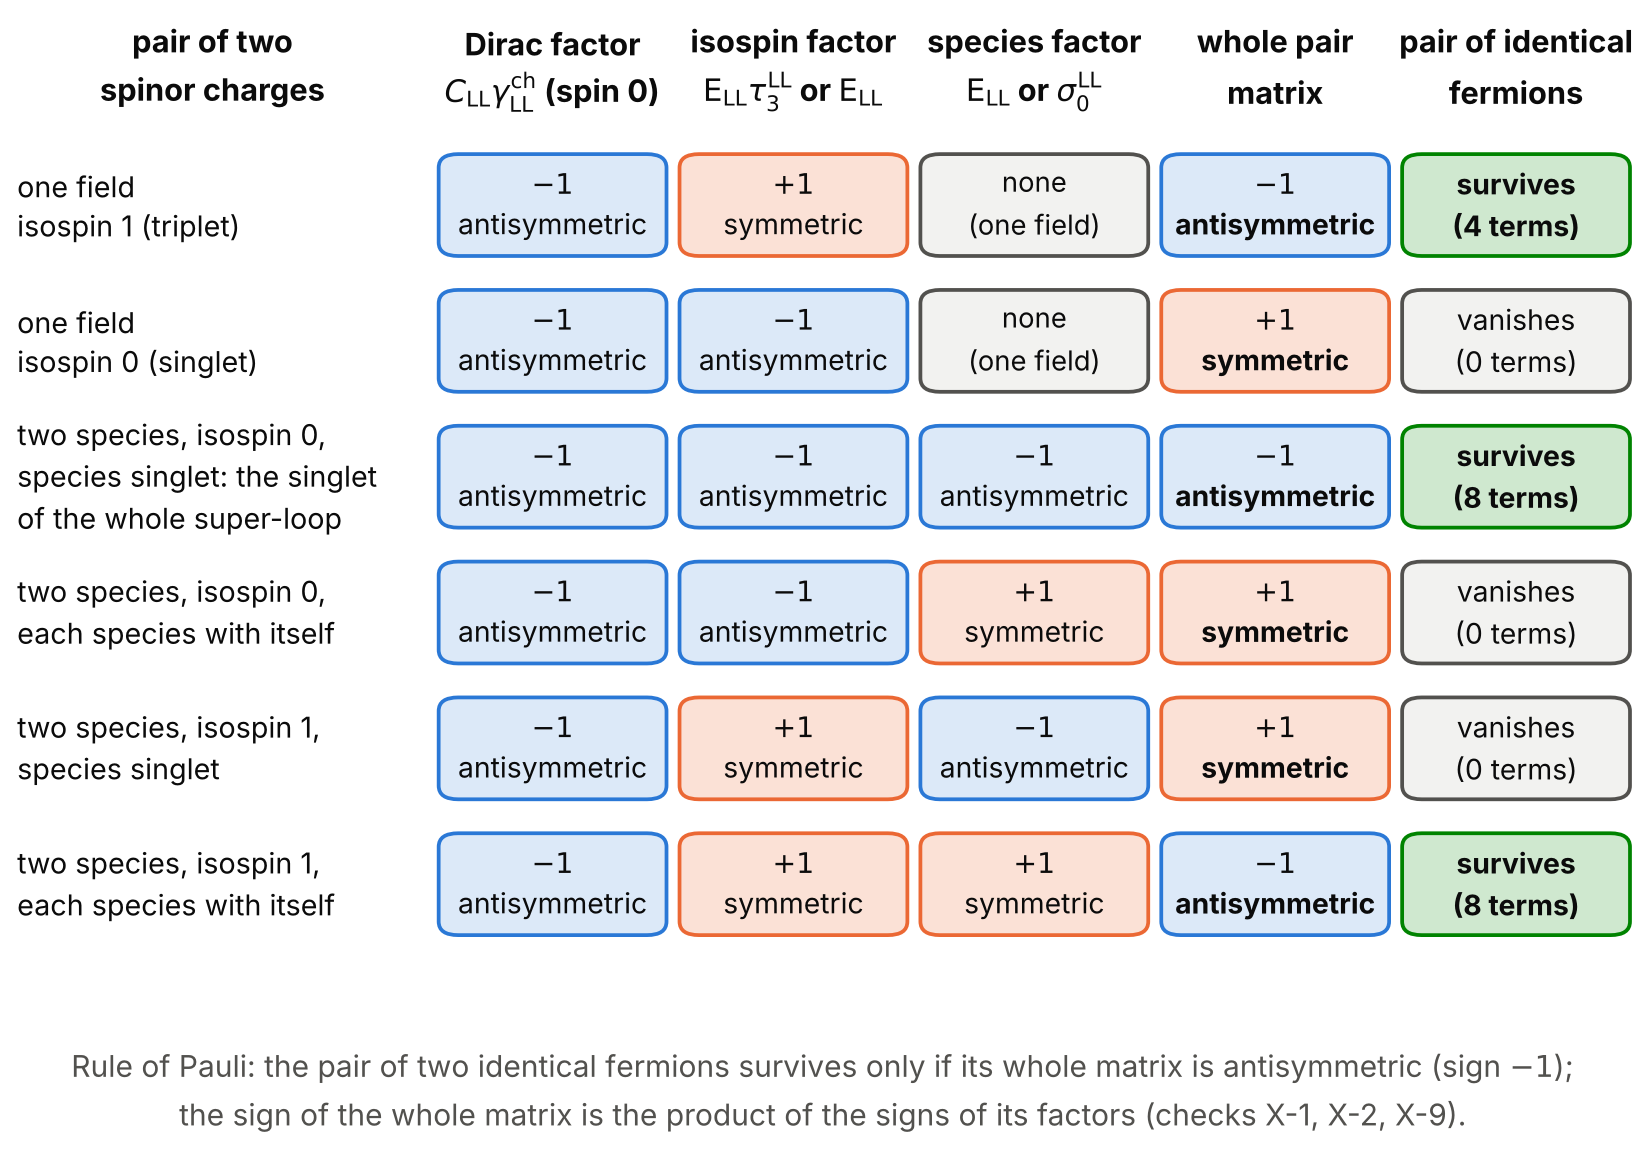
\includegraphics[width=1\textwidth,height=\textheight]{figures/fig_ex_bookkeeping.png}

\textbf{Figure 1.} The rule of Pauli as a bookkeeping of signs. Each row
is a pair of two spinor charges in an s-wave. The columns give the
exchange sign (\(+1\) symmetric, \(-1\) antisymmetric) of the Dirac
factor (here always \(C_{\rm LL}\gamma^{\rm ch}_{\rm LL}\), spin 0), of
the isospin factor (\(\mathsf E_{\rm LL}\tau^{\rm LL}_3\), isospin 1, or
\(\mathsf E_{\rm LL}\), isospin 0), of the species factor (none for one
field; \(\mathsf E_{\rm LL}\), the species singlet, or
\(\sigma^{\rm LL}_0\), each species paired with itself), and of the
whole pair matrix, which is the product of the three. Blue: sign \(-1\);
orange: sign \(+1\); grey: no species factor. Identical fermions need
the sign \(-1\) for the whole matrix; the last column states whether the
pair survives and how many independent terms it keeps. For one field
only the isospin triplet survives (first row). The singlet of the whole
super-loop, spin 0 and isospin 0, survives only with two species in the
species singlet (third row). Data:
\texttt{explanations/data/ex\_pair\_matrices.csv}; checks X-1, X-2, X-9;
drawn by \texttt{explanations/code/make\_explain\_figures.py}.

\hypertarget{comparison-with-the-nucleons}{%
\subsection{5.4 Comparison with the
nucleons}\label{comparison-with-the-nucleons}}

The ¹S₀ pairs of nucleons and the spin-zero pairs of the spinor charges
have the same structure: spin 0, isospin 1, three charge states. The
difference is the electric charge of the members of the doublet. For
nucleons the charge is the isospin projection plus one half of the
baryon number (proton 1, neutron 0), so the three pairs have the charges
2, 1, 0 in units of the proton charge. For the spinor charges the charge
is \(Q_{\rm LL}=T^3_{\rm LL}\) alone (up \(+\tfrac12\), down
\(-\tfrac12\)), so the three pairs have the charges \(+1\), 0, \(-1\),
and the pair with the charge 0 is the up-down pair.

\hypertarget{superfluid-condenses-what-forms-and-why}{%
\section{6. ``Superfluid \ldots{} condenses'': what forms, and
why}\label{superfluid-condenses-what-forms-and-why}}

\hypertarget{the-hamiltonian}{%
\subsection{6.1 The Hamiltonian}\label{the-hamiltonian}}

The manuscript studies free Dirac particles of mass \(m_{\rm LL}\) at
the chemical potential \(\mu_{\rm LL}\), with an attractive contact
interaction in the scalar spin-zero channels,
\[\mathcal H^{\rm sf}_{\rm LL}=\sum_{\vec q_{\rm LL}}\Psi^\dagger_{\rm LL}\big(\mathsf h_{\rm LL}-\mu_{\rm LL}\big)\Psi_{\rm LL}-\tfrac14G_{\rm LL}\sum_\iota\big(\Pi^\iota_{\rm LL}\big)^\dagger\Pi^\iota_{\rm LL}, \tag{6.1}\]
with the pair operators of the three scalar channels
\[\Pi^\iota_{\rm LL}=\sum_{\vec q_{\rm LL}}\Psi_{\rm LL}(\vec q_{\rm LL})^T\,\mathsf K^\iota_{\rm LL}\,\Psi_{\rm LL}(-\vec q_{\rm LL}), \tag{6.2}\]
which annihilate two spinor charges of opposite momenta. All momentum
sums run over \(q_{\rm LL}<\Lambda_{\rm LL}\). The \textbf{chemical
potential} \(\mu_{\rm LL}\) is the energy needed to add one particle;
for \(\mu_{\rm LL}>m_{\rm LL}\) the normal state is a filled Fermi sea
of particles up to the \textbf{Fermi momentum}
\(k^{\rm F}_{\rm LL}=(\mu_{\rm LL}^2-m_{\rm LL}^2)^{1/2}\). The
\textbf{coupling} \(G_{\rm LL}>0\) makes the interaction attractive. The
sum over \(\iota\) is the scalar product of two isospin vectors, so the
interaction is isospin invariant: it attracts the up-up, up-down and
down-down pairs equally.

\hypertarget{the-order-parameter}{%
\subsection{6.2 The order parameter}\label{the-order-parameter}}

The \textbf{order parameter} is the complex isospin vector
\(\vec d_{\rm LL}=(d^1_{\rm LL},d^2_{\rm LL},d^3_{\rm LL})\),
\[d^\iota_{\rm LL}=-\tfrac12G_{\rm LL}\,\langle\Pi^\iota_{\rm LL}\rangle , \tag{6.3}\]
the expectation value of the pair operators in the ground state, times
\(-\tfrac12G_{\rm LL}\). In the normal state it is zero: the ground
state of a fixed number of particles gives zero for an operator that
removes two particles. A ground state with \(\vec d_{\rm LL}\neq0\) is a
coherent superposition of states with different numbers of pairs, in
which a macroscopic number of pairs share one pair wavefunction: a
\textbf{condensate} of pairs. Because the three pair matrices
\(\mathsf K^\iota_{\rm LL}\) transform under isospin rotations like the
components of a vector, so does \(\vec d_{\rm LL}\). Under the
transformation \(\Psi_{\rm LL}\to e^{i\theta_{\rm LL}}\Psi_{\rm LL}\)
generated by the \textbf{fermion number} \(F_{\rm LL}\), the pair
operators change by \(e^{2i\theta_{\rm LL}}\), and so does
\(\vec d_{\rm LL}\).

\hypertarget{mean-field-and-the-wavefunction-of-the-condensed-pairs}{%
\subsection{6.3 Mean field, and the wavefunction of the condensed
pairs}\label{mean-field-and-the-wavefunction-of-the-condensed-pairs}}

In the \textbf{mean-field approximation} each product of pair operators
in Eq. (6.1) is replaced by
\[-\tfrac14G_{\rm LL}\big[\langle\Pi^\iota_{\rm LL}\rangle^*\,\Pi^\iota_{\rm LL}+(\Pi^\iota_{\rm LL})^\dagger\langle\Pi^\iota_{\rm LL}\rangle-\lvert\langle\Pi^\iota_{\rm LL}\rangle\rvert^2\big]=\tfrac12d^{\iota*}_{\rm LL}\Pi^\iota_{\rm LL}+\tfrac12d^\iota_{\rm LL}(\Pi^\iota_{\rm LL})^\dagger+\frac{\lvert d^\iota_{\rm LL}\rvert^2}{G_{\rm LL}} ,\]
which neglects only the fluctuations of the pair operators about their
mean values. The term
\[\tfrac12\sum_\iota d^\iota_{\rm LL}(\Pi^\iota_{\rm LL})^\dagger=\tfrac12\sum_{\vec q_{\rm LL}}\Psi^\dagger_{\rm LL}(\vec q_{\rm LL})\,\mathsf P_{\rm LL}\,\Psi^\dagger_{\rm LL}(-\vec q_{\rm LL})^T,\qquad\mathsf P_{\rm LL}=\sum_\iota d^\iota_{\rm LL}(\mathsf K^\iota_{\rm LL})^\dagger ,\]
creates pairs with the pair matrix \(\mathsf P_{\rm LL}\). Because
\((\mathsf K^\iota_{\rm LL})^\dagger=(C_{\rm LL}\gamma^{\rm ch}_{\rm LL})^\dagger\otimes(\mathsf E_{\rm LL}\tau^{\rm LL}_\iota)^\dagger\),
\[\mathsf P_{\rm LL}=\big(C_{\rm LL}\gamma^{\rm ch}_{\rm LL}\big)^\dagger\otimes\mathsf D_{\rm LL},\qquad\mathsf D_{\rm LL}=\sum_\iota d^\iota_{\rm LL}\big(\mathsf E_{\rm LL}\tau^{\rm LL}_\iota\big)^\dagger=\begin{pmatrix}d^1_{\rm LL}-i\,d^2_{\rm LL}&-d^3_{\rm LL}\\-d^3_{\rm LL}&-d^1_{\rm LL}-i\,d^2_{\rm LL}\end{pmatrix}. \tag{6.4}\]
In the ground state of the mean-field Hamiltonian the pairs are created
with this matrix: for one pair of momenta the ground state is a
superposition of ``no pair'' and ``one pair'', and the ratio of the two
amplitudes is a negative number times the coefficient of the pair term.
\textbf{The condensed pairs therefore have the spin factor
\((C_{\rm LL}\gamma^{\rm ch}_{\rm LL})^\dagger\) (spin 0) and the
isospin wavefunction \(\mathsf D_{\rm LL}\)}: the entry of
\(\mathsf D_{\rm LL}\) in the row of the isospin of one particle and the
column of the isospin of the other is the amplitude of that combination
(check X-5 verifies that this matrix equals
\(-\sum_\iota d^\iota_{\rm LL}\tau^{\rm LL}_\iota\mathsf E_{\rm LL}\),
the form used to compute the pair content).

The mean-field Hamiltonian is quadratic in the field. For each momentum
it is described by the \(16\times16\) \textbf{Bogoliubov-de Gennes
matrix}
\[\mathsf H_{\rm LL}=\begin{pmatrix}\mathsf h_{\rm LL}(\vec q_{\rm LL})-\mu_{\rm LL}&\mathsf P_{\rm LL}\\\mathsf P_{\rm LL}^\dagger&-\big(\mathsf h_{\rm LL}(-\vec q_{\rm LL})-\mu_{\rm LL}\big)^T\end{pmatrix}\]
acting on the Nambu spinor
\(\mathcal N_{\rm LL}=(\Psi_{\rm LL}(\vec q_{\rm LL}),\Psi^*_{\rm LL}(-\vec q_{\rm LL}))\),
which combines the annihilation of a particle with the creation of its
partner. Its positive eigenvalues are the energies of the
quasi-particles (Bogoliubov quasi-particles: superpositions of a
particle and a hole). Section 7 shows that they are
\[E^\pm_{\rm LL}=\big[(\varepsilon_{\rm LL}\pm\mu_{\rm LL})^2+\Delta_{\rm LL}^2\big]^{1/2}, \tag{6.5}\]
with the \textbf{gap} \(\Delta_{\rm LL}\) in place of each of the two
gaps of the state. \(E^-_{\rm LL}\) is the branch of the particles near
the Fermi surface; its minimum, at \(q_{\rm LL}=k^{\rm F}_{\rm LL}\), is
the gap itself: every excitation costs at least \(\Delta_{\rm LL}\).
\(E^+_{\rm LL}\) is the antiparticle branch.

\hypertarget{condensation-the-grand-potential-and-the-gap-equation}{%
\subsection{6.4 Condensation: the grand potential and the gap
equation}\label{condensation-the-grand-potential-and-the-gap-equation}}

The \textbf{grand potential} per volume at zero temperature, measured
from the normal state, is
\[\Omega_{\rm LL}=\frac{\lvert\vec d_{\rm LL}\rvert^2}{G_{\rm LL}}-\frac12\int\!\frac{d^3q_{\rm LL}}{(2\pi)^3}\sum\big(\text{positive eigenvalues of }\mathsf H_{\rm LL}\big)-\big(\text{the same at }\vec d_{\rm LL}=0\big). \tag{6.6}\]
``\textbf{Condenses}'' means: the minimum of \(\Omega_{\rm LL}\) lies at
\(\vec d_{\rm LL}\neq0\), so that the condensate has a lower grand
potential than the normal state. For a unitary state (Section 7), with
the single gap \(\Delta_{\rm LL}=\lvert\vec d_{\rm LL}\rvert\), each of
the energies (6.5) occurs twice among the eight positive eigenvalues,
and setting the derivative of \(\Omega_{\rm LL}\) with respect to
\(\Delta_{\rm LL}^2\) to zero gives the \textbf{gap equation}
\[\frac1{G_{\rm LL}}=\int_{q_{\rm LL}<\Lambda_{\rm LL}}\frac{d^3q_{\rm LL}}{(2\pi)^3}\Big(\frac1{E^+_{\rm LL}}+\frac1{E^-_{\rm LL}}\Big). \tag{6.7}\]
There are two regimes.

\begin{itemize}
\tightlist
\item
  \textbf{Vacuum} (\(\mu_{\rm LL}=0\)). As \(\Delta_{\rm LL}\to0\) the
  right side tends to a finite value, so a gap appears only above the
  \textbf{critical coupling}
  \[G^{\rm crit}_{\rm LL}=\frac{2\pi^2}{\Lambda_{\rm LL}(\Lambda_{\rm LL}^2+m_{\rm LL}^2)^{1/2}-m_{\rm LL}^2\ln\big[(\Lambda_{\rm LL}+(\Lambda_{\rm LL}^2+m_{\rm LL}^2)^{1/2})/m_{\rm LL}\big]},\]
  which is \(2\pi^2/\Lambda_{\rm LL}^2={}19.739209\) for
  \(m_{\rm LL}=0\) and \(21.286610\) for \(m_{\rm LL}=0.2\).
\item
  \textbf{A Fermi sea} (\(\mu_{\rm LL}>m_{\rm LL}\)). The integral of
  \(1/E^-_{\rm LL}\) diverges logarithmically as
  \(\Delta_{\rm LL}\to0\), because \(E^-_{\rm LL}\) vanishes at the
  Fermi surface. The gap equation then has a solution for \textbf{every}
  positive coupling (the instability found by Cooper). At weak coupling
  \(\ln\Delta_{\rm LL}\) is a linear function of \(1/G_{\rm LL}\) with
  the slope
  \(-1/(2\nu^{\rm F}_{\rm LL})=-\pi^2/(k^{\rm F}_{\rm LL}\mu_{\rm LL})\),
  where \(\nu^{\rm F}_{\rm LL}=k^{\rm F}_{\rm LL}\mu_{\rm LL}/(2\pi^2)\)
  is the density of states of one species and one spin state at the
  Fermi surface: the law of Bardeen, Cooper and Schrieffer. For
  \(\mu_{\rm LL}=0.5\), \(m_{\rm LL}=0.2\) the computed slope is
  \(-43.0637\), against \(-43.0745\) from the formula (ratio
  \(0.9997\)).
\end{itemize}

The example used in the rest of this document is \(G_{\rm LL}=12\),
\(\mu_{\rm LL}=0.5\), \(m_{\rm LL}=0.2\). This coupling is below the
critical coupling of the vacuum, yet the Fermi sea condenses: the gap is
\(\Delta_{\rm LL}={}0.090417\) and the minimum of the grand potential is
\(\Omega_{\rm LL}={}-9.720605\times10^{-5}\). (These numbers come from
the program \texttt{superloop}; its report is printed in Section 11.4.)

\hypertarget{why-the-condensate-is-a-superfluid}{%
\subsection{6.5 Why the condensate is a
superfluid}\label{why-the-condensate-is-a-superfluid}}

A non-zero \(\vec d_{\rm LL}\) is not unchanged by the fermion-number
transformation: it is multiplied by \(e^{2i\theta_{\rm LL}}\). The
condensate therefore has a definite phase and an indefinite number of
particles; the symmetry \(U(1)^{\rm F}_{\rm LL}\) generated by
\(F_{\rm LL}\) is broken. This is the defining property of a superfluid,
as in helium 4 (the phase of a condensate of bosons), in helium 3 and in
the neutron superfluid of neutron stars (the phase of a condensate of
fermion pairs). A slow twist of the phase in space is a current of
particles; it cannot decay by scattering single particles, because every
quasi-particle costs at least the gap: the current flows without
friction. The manuscript computes the mean-field ground state at zero
temperature; ``superfluid'' names this condensate with the broken
fermion number. \textbf{A spin-zero superfluid is a superfluid whose
condensed pairs have spin 0.}

\hypertarget{unitary}{%
\section{7. ``Unitary''}\label{unitary}}

\hypertarget{the-two-gaps-of-a-condensate}{%
\subsection{7.1 The two gaps of a
condensate}\label{the-two-gaps-of-a-condensate}}

Multiplying the matrix \(\mathsf D_{\rm LL}\) of Eq. (6.4) by its
Hermitian conjugate gives
\[\mathsf D_{\rm LL}\mathsf D_{\rm LL}^\dagger=\lvert\vec d_{\rm LL}\rvert^2\,\sigma^{\rm LL}_0+i\sum_\iota\big(\vec d_{\rm LL}\times\vec d^{\,*}_{\rm LL}\big)^\iota\,\tau^{\rm LL}_\iota . \tag{7.1}\]
For example, its entry in the first row and column is
\(\lvert d^1_{\rm LL}-i\,d^2_{\rm LL}\rvert^2+\lvert d^3_{\rm LL}\rvert^2=\lvert\vec d_{\rm LL}\rvert^2+i\,(d^1_{\rm LL}d^{2*}_{\rm LL}-d^2_{\rm LL}d^{1*}_{\rm LL})\),
and \(d^1_{\rm LL}d^{2*}_{\rm LL}-d^2_{\rm LL}d^{1*}_{\rm LL}\) is the
third component of \(\vec d_{\rm LL}\times\vec d^{\,*}_{\rm LL}\). The
vector \(i\,\vec d_{\rm LL}\times\vec d^{\,*}_{\rm LL}\) is real (it
equals its own complex conjugate), so the eigenvalues of (7.1) are
\(\lvert\vec d_{\rm LL}\rvert^2\) plus or minus its length. A unitary
change of basis in the space of the holes brings the Bogoliubov-de
Gennes matrix to two blocks, one for each eigenvalue, whose squares are
\((\mathsf h_{\rm LL}-\mu_{\rm LL})^2\) plus that eigenvalue; hence the
energies (6.5) for the \textbf{two gaps}
\[(\Delta^\pm_{\rm LL})^2=\lvert\vec d_{\rm LL}\rvert^2\,(1\pm\zeta_{\rm LL}),\qquad\zeta_{\rm LL}=\frac{\lvert\vec d_{\rm LL}\times\vec d^{\,*}_{\rm LL}\rvert}{\lvert\vec d_{\rm LL}\rvert^2}=\Big(1-\frac{\lvert\sum_\iota(d^\iota_{\rm LL})^2\rvert^2}{\lvert\vec d_{\rm LL}\rvert^4}\Big)^{1/2}. \tag{7.2}\]
The second form of the \textbf{non-unitarity} \(\zeta_{\rm LL}\) follows
from the identity
\(\lvert\vec d_{\rm LL}\times\vec d^{\,*}_{\rm LL}\rvert^2=\lvert\vec d_{\rm LL}\rvert^4-\lvert\sum_\iota(d^\iota_{\rm LL})^2\rvert^2\)
(the identity of Binet and Cauchy for the cross product). Always
\(0\le\zeta_{\rm LL}\le1\). The program verifies Eq. (7.2) for the seven
examples below and for 200 random order parameters (check X-6).

\textbf{Definition.} A condensate is \textbf{unitary} if
\(\zeta_{\rm LL}=0\). The following statements are equivalent:

\begin{itemize}
\tightlist
\item
  \(\zeta_{\rm LL}=0\), that is,
  \(\vec d_{\rm LL}\times\vec d^{\,*}_{\rm LL}=0\);
\item
  \(\mathsf D_{\rm LL}\mathsf D_{\rm LL}^\dagger=\lvert\vec d_{\rm LL}\rvert^2\sigma^{\rm LL}_0\):
  the gap matrix divided by \(\lvert\vec d_{\rm LL}\rvert\) is a
  \textbf{unitary matrix}, which is the origin of the name (it comes
  from the theory of superfluid helium 3);
\item
  \(\vec d_{\rm LL}\) is a complex number times a real vector,
  \(\vec d_{\rm LL}=e^{i\theta_{\rm LL}}\lvert\vec d_{\rm LL}\rvert\)
  times a real unit vector (because
  \(\lvert\sum_\iota(d^\iota_{\rm LL})^2\rvert\le\sum_\iota\lvert d^\iota_{\rm LL}\rvert^2\),
  with equality exactly when all components have the same phase up to a
  sign);
\item
  both isospin directions have the same gap,
  \(\Delta^+_{\rm LL}=\Delta^-_{\rm LL}=\lvert\vec d_{\rm LL}\rvert\):
  every particle, up or down, is paired with the same strength;
\item
  the average isospin of a condensed pair is zero (Section 7.2).
\end{itemize}

A condensate with \(\zeta_{\rm LL}>0\) is \textbf{non-unitary}: it pairs
the two isospin directions unequally. In the \textbf{fully non-unitary}
case \(\zeta_{\rm LL}=1\) the gaps are
\(\sqrt2\,\lvert\vec d_{\rm LL}\rvert\) and 0: one isospin direction is
not paired at all.

\hypertarget{what-the-condensed-pairs-are-made-of}{%
\subsection{7.2 What the condensed pairs are made
of}\label{what-the-condensed-pairs-are-made-of}}

By Eq. (6.4) the condensed pairs have the amplitude
\(d^1_{\rm LL}-i\,d^2_{\rm LL}\) for up with up (charge \(+1\)),
\(-d^3_{\rm LL}\) for up with down and the same for down with up (charge
0), and \(-d^1_{\rm LL}-i\,d^2_{\rm LL}\) for down with down (charge
\(-1\)). The squares of these amplitudes add up to
\(2\lvert\vec d_{\rm LL}\rvert^2\). The \textbf{fractions of the pairs
with the charges \(+1\), 0 and \(-1\)} are therefore
\[\frac{\lvert d^1_{\rm LL}-i\,d^2_{\rm LL}\rvert^2}{2\lvert\vec d_{\rm LL}\rvert^2},\qquad\frac{\lvert d^3_{\rm LL}\rvert^2}{\lvert\vec d_{\rm LL}\rvert^2},\qquad\frac{\lvert d^1_{\rm LL}+i\,d^2_{\rm LL}\rvert^2}{2\lvert\vec d_{\rm LL}\rvert^2}. \tag{7.3}\]
They are probabilities: the probability that a measurement of the charge
of one condensed pair gives \(+1\), 0 or \(-1\). The \textbf{average
charge of a pair} is the first minus the third; expanding the squares
gives
\[\frac{\lvert d^1_{\rm LL}-i\,d^2_{\rm LL}\rvert^2-\lvert d^1_{\rm LL}+i\,d^2_{\rm LL}\rvert^2}{2\lvert\vec d_{\rm LL}\rvert^2}=\frac{i\,(d^1_{\rm LL}d^{2*}_{\rm LL}-d^2_{\rm LL}d^{1*}_{\rm LL})}{\lvert\vec d_{\rm LL}\rvert^2}=\frac{i\,(\vec d_{\rm LL}\times\vec d^{\,*}_{\rm LL})^3}{\lvert\vec d_{\rm LL}\rvert^2}. \tag{7.4}\]
The charge is the third component of the isospin. Both the average
isospin of a pair and the vector
\(i\,\vec d_{\rm LL}\times\vec d^{\,*}_{\rm LL}/\lvert\vec d_{\rm LL}\rvert^2\)
turn like vectors under isospin rotations, and their third components
agree for every \(\vec d_{\rm LL}\); rotating any direction into the
third, all components agree:
\[\text{average isospin of a condensed pair}=\frac{i\,\vec d_{\rm LL}\times\vec d^{\,*}_{\rm LL}}{\lvert\vec d_{\rm LL}\rvert^2},\qquad\text{its length}=\zeta_{\rm LL}. \tag{7.5}\]
(The program computes the average isospin directly from the pair
wavefunction and compares, check X-5.) Hence \textbf{a condensate is
unitary exactly when the average isospin of its pairs is zero; in
particular, the average electric charge of the pairs of a unitary
condensate is zero.} At the other extreme, \(\zeta_{\rm LL}=1\) means
that the average isospin has the length 1, the largest possible for
isospin 1: every pair has the isospin projection \(+1\) on one axis, for
example every pair is up-up.

\hypertarget{seven-examples}{%
\subsection{7.3 Seven examples}\label{seven-examples}}

The program computes the content of seven example condensates (data file
\texttt{explanations/data/ex\_states.csv}, checks X-5 to X-7). All have
\(\lvert\vec d_{\rm LL}\rvert=1\), so the gaps are in units of
\(\lvert\vec d_{\rm LL}\rvert\):

\sptkeptpenalty=10000
\begin{longtable}[]{@{}
  >{\raggedright\arraybackslash}p{(\columnwidth - 14\tabcolsep) * \real{0.1200}}
  >{\raggedright\arraybackslash}p{(\columnwidth - 14\tabcolsep) * \real{0.2300}}
  >{\raggedright\arraybackslash}p{(\columnwidth - 14\tabcolsep) * \real{0.1300}}
  >{\raggedright\arraybackslash}p{(\columnwidth - 14\tabcolsep) * \real{0.0800}}
  >{\raggedright\arraybackslash}p{(\columnwidth - 14\tabcolsep) * \real{0.0500}}
  >{\raggedright\arraybackslash}p{(\columnwidth - 14\tabcolsep) * \real{0.1000}}
  >{\raggedright\arraybackslash}p{(\columnwidth - 14\tabcolsep) * \real{0.0900}}
  >{\raggedright\arraybackslash}p{(\columnwidth - 14\tabcolsep) * \real{0.2000}}@{}}
\toprule\noalign{}
\begin{minipage}[b]{\linewidth}\raggedright
example
\end{minipage} & \begin{minipage}[b]{\linewidth}\raggedright
\(\vec d_{\rm LL}\)
\end{minipage} & \begin{minipage}[b]{\linewidth}\raggedright
fractions of pairs with charge \(+1\), 0, \(-1\)
\end{minipage} & \begin{minipage}[b]{\linewidth}\raggedright
average charge of a pair
\end{minipage} & \begin{minipage}[b]{\linewidth}\raggedright
\(\zeta_{\rm LL}\)
\end{minipage} & \begin{minipage}[b]{\linewidth}\raggedright
gaps \(\Delta^+_{\rm LL}\), \(\Delta^-_{\rm LL}\) in units of
\(\lvert\vec d_{\rm LL}\rvert\)
\end{minipage} & \begin{minipage}[b]{\linewidth}\raggedright
unpaired
\end{minipage} & \begin{minipage}[b]{\linewidth}\raggedright
unbroken generator
\end{minipage} \\
\midrule\noalign{}
\endhead
\bottomrule\noalign{}
\endlastfoot
polar along the third axis & \((0,0,1)\) & 0, 1, 0 & 0 & 0 & 1, 1 & none
& isospin rotation about the axis (0, 0, 1):
\(T^3_{\rm LL}=Q_{\rm LL}\) \\*
polar along the first axis & \((1,0,0)\) & 0.5, 0, 0.5 & 0 & 0 & 1, 1 &
none & isospin rotation about the axis (1, 0, 0) \\*
polar along (1,2,2)/3 & \((1,2,2)/3\) & 0.277778, 0.444444, 0.277778 & 0
& 0 & 1, 1 & none & isospin rotation about the axis (0.333333, 0.666667,
0.666667) \\*
unitary with a phase & \(\exp(i\pi/4)\,(0,0.6,0.8)\) & 0.18, 0.64, 0.18
& 0 & 0 & 1, 1 & none & isospin rotation about the axis (0, 0.6, 0.8) \\*
partly non-unitary & \((1,i/2,0)/\sqrt{5/4}\) & 0.9, 0, 0.1 & 0.8 & 0.8
& 1.341641, 0.447214 & none & none \\*
charged, up-up pairs & \((1,i,0)/\sqrt2\) & 1, 0, 0 & 1 & 1 & 1.414214,
0 & isospin down & \(\tfrac12F_{\rm LL}-T^3_{\rm LL}\), the number of
isospin-down particles \\*
charged, down-down pairs & \((1,-i,0)/\sqrt2\) & 0, 0, 1 & \(-1\) & 1 &
1.414214, 0 & isospin up & \(\tfrac12F_{\rm LL}+T^3_{\rm LL}\), the
number of isospin-up particles \\
\end{longtable}

The entries can be checked by hand with Eqs. (6.4), (7.2) and (7.3):

\begin{enumerate}
\def\labelenumi{\arabic{enumi}.}
\tightlist
\item
  \emph{Polar along the third axis}, \(\vec d_{\rm LL}=(0,0,1)\).
  \(\mathsf D_{\rm LL}\) has only the two entries \(-1\) off the
  diagonal: every pair is
  \((\lvert\uparrow\downarrow\rangle+\lvert\downarrow\uparrow\rangle)/\sqrt2\),
  of charge 0. Unitary, both gaps 1. This is the ground state named in
  the manuscript.
\item
  \emph{Polar along the first axis}, \(\vec d_{\rm LL}=(1,0,0)\).
  \(\mathsf D_{\rm LL}=\mathrm{diag}(1,-1)\): every pair is
  \((\lvert\uparrow\uparrow\rangle-\lvert\downarrow\downarrow\rangle)/\sqrt2\).
  A measurement of the charge of one pair gives \(+1\) or \(-1\) with
  the probability \(\tfrac12\) each; no pair has a definite charge, but
  the average is 0. Unitary, both gaps 1.
\item
  \emph{Polar along \((1,2,2)/3\)}. The fractions are
  \(\lvert\tfrac13-\tfrac23i\rvert^2/2=\tfrac5{18}\),
  \((\tfrac23)^2=\tfrac49\) and \(\tfrac5{18}\); the average charge is
  0. Unitary.
\item
  \emph{Unitary with a phase},
  \(\vec d_{\rm LL}=\exp(i\pi/4)\,(0,0.6,0.8)\). A common phase of all
  components changes nothing in Eqs. (7.2) to (7.5): the fractions are
  \(0.6^2/2=0.18\), \(0.8^2=0.64\) and \(0.18\), the average charge is
  0, and the state is unitary. (The common phase is the phase of the
  condensate of Section 6.5.)
\item
  \emph{Partly non-unitary}, \(\vec d_{\rm LL}=(1,i/2,0)/\sqrt{5/4}\).
  Here
  \(\sum_\iota(d^\iota_{\rm LL})^2=(1-\tfrac14)\cdot\tfrac45=\tfrac35\),
  so \(\zeta_{\rm LL}=(1-\tfrac9{25})^{1/2}=\tfrac45\). The fractions
  are \(\tfrac9{10}\), 0, \(\tfrac1{10}\); the average charge is
  \(\tfrac45=\zeta_{\rm LL}\); the gaps are \((\tfrac95)^{1/2}\) and
  \((\tfrac15)^{1/2}\).
\item
  \emph{Charged, up-up pairs}, \(\vec d_{\rm LL}=(1,i,0)/\sqrt2\). Here
  \(\sum_\iota(d^\iota_{\rm LL})^2=0\), so \(\zeta_{\rm LL}=1\), and
  \(\mathsf D_{\rm LL}\) has the single entry \(\sqrt2\) in the up-up
  place: every pair consists of two up particles and has the charge
  \(+1\). The up particles are paired with the larger gap \(\sqrt2\);
  the down particles are not paired at all: their energies are those of
  free particles, \(\lvert\varepsilon_{\rm LL}-\mu_{\rm LL}\rvert\),
  which vanish at the Fermi surface.
\item
  \emph{Charged, down-down pairs}, \(\vec d_{\rm LL}=(1,-i,0)/\sqrt2\):
  the mirror image, pairs of charge \(-1\), the up particles unpaired.
\end{enumerate}

The numbers in the table, computed in double precision, agree with these
exact values.

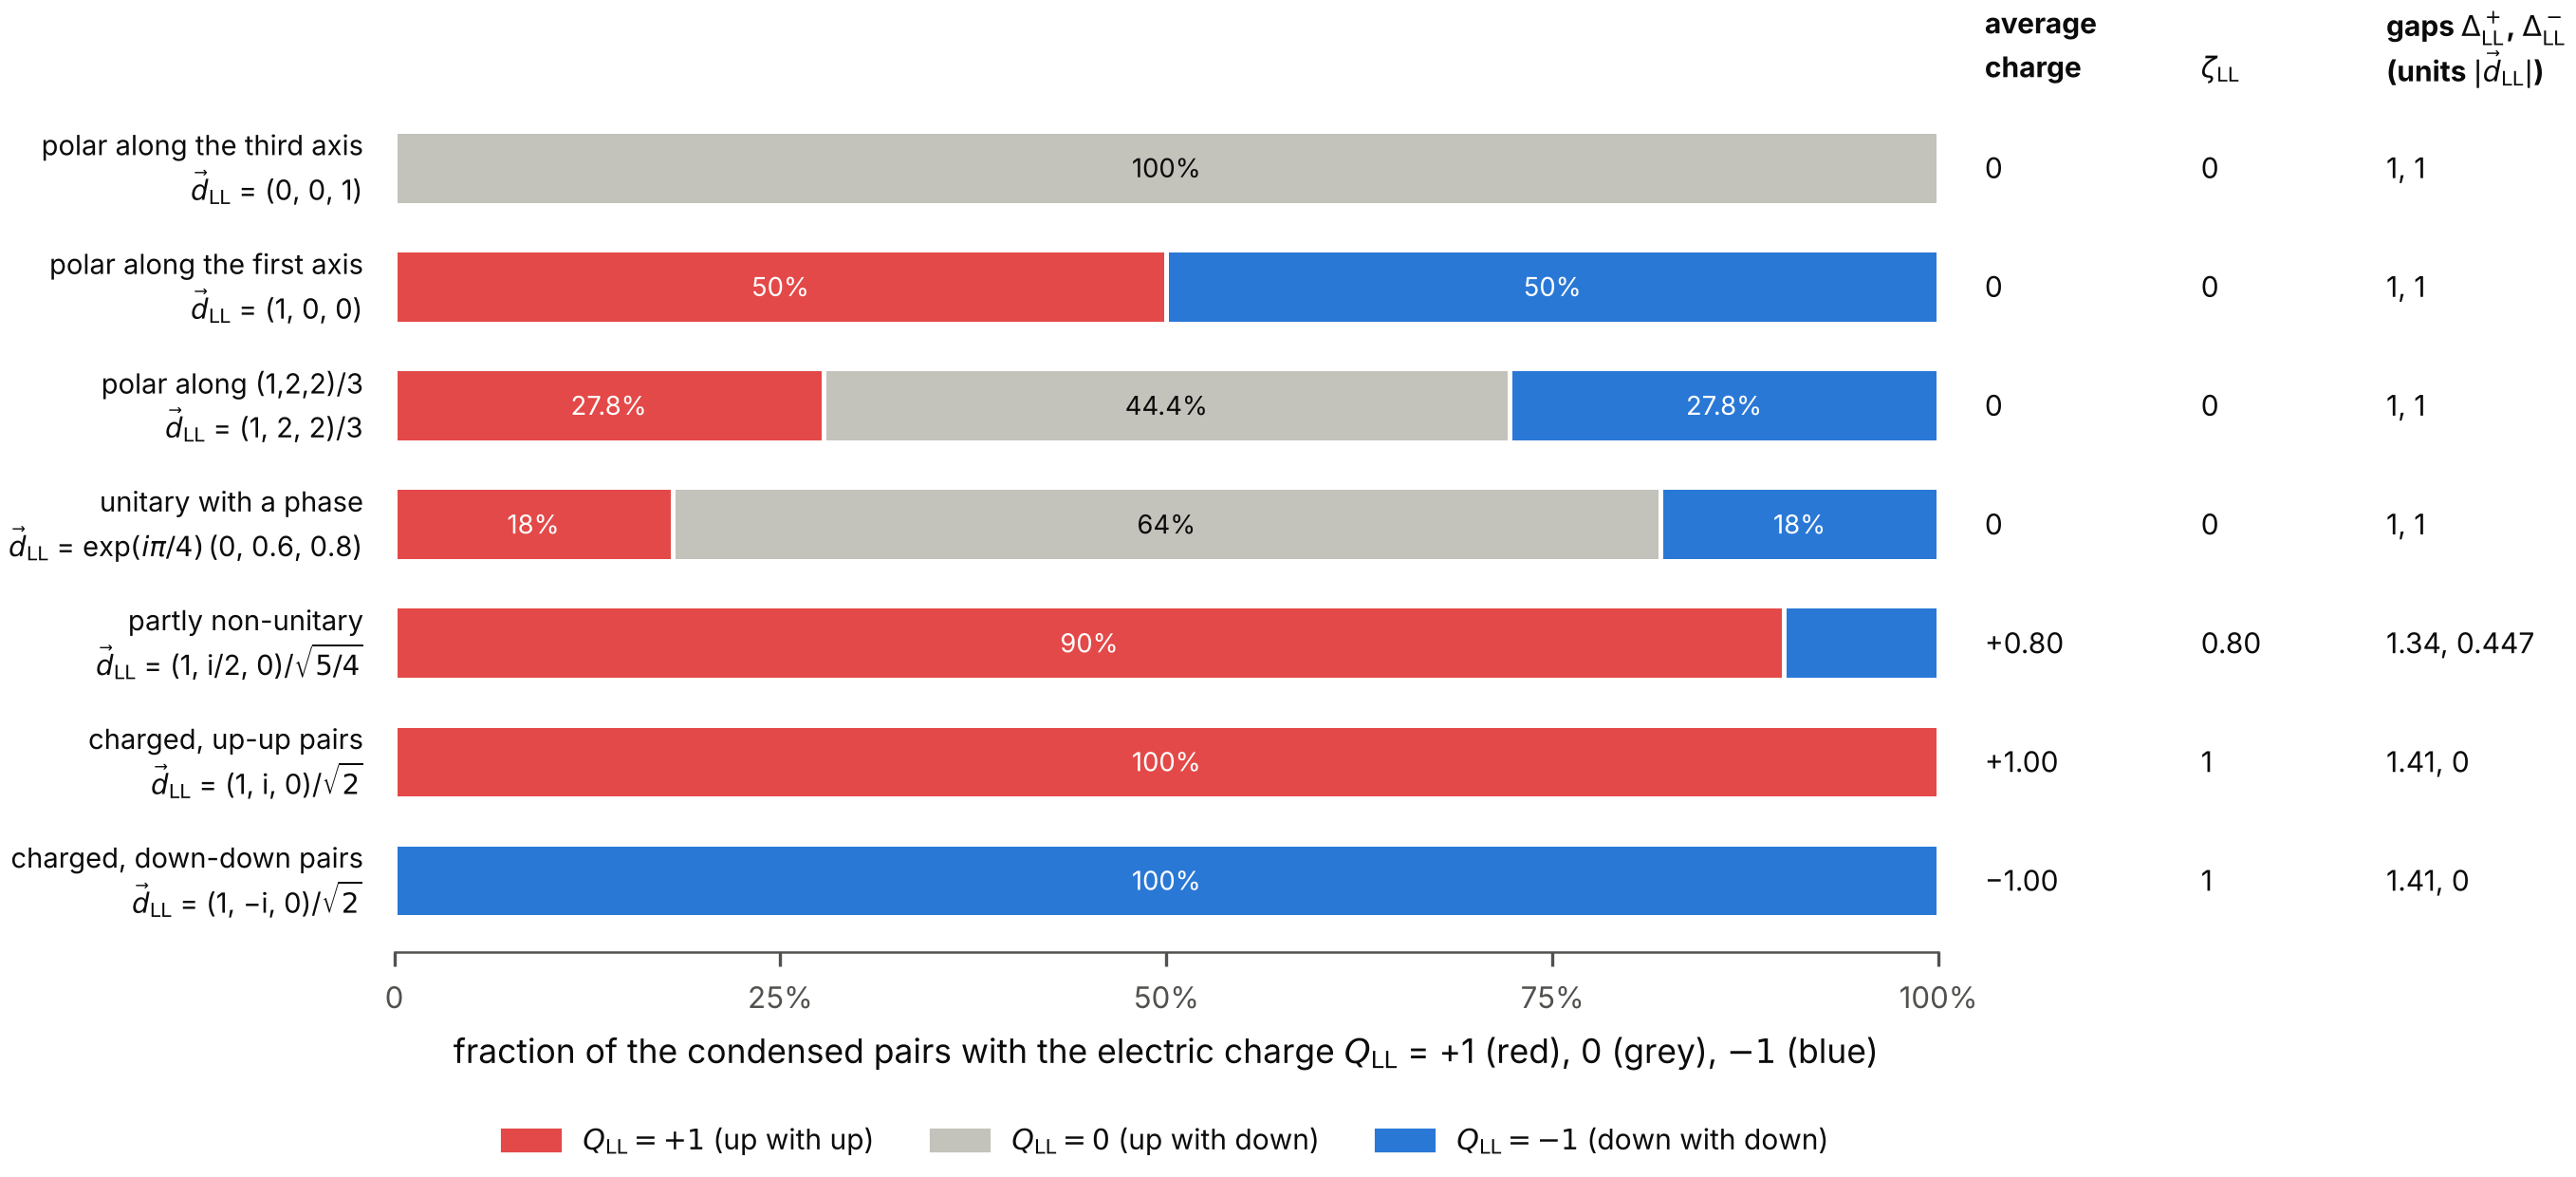
\includegraphics[width=1\textwidth,height=\textheight]{figures/fig_ex_pairs.png}

\textbf{Figure 2.} What the condensed pairs of the seven example
condensates are made of. Each bar divides the condensed pairs into those
of the charge \(+1\) (two isospin-up particles, red), 0 (one up and one
down, grey) and \(-1\) (two isospin-down particles, blue), Eq. (7.3). To
the right: the average charge of a pair, Eq. (7.4), the non-unitarity
\(\zeta_{\rm LL}\), and the two gaps in units of
\(\lvert\vec d_{\rm LL}\rvert\). The four unitary condensates
(\(\zeta_{\rm LL}=0\)) have pairs of average charge 0 and one gap for
both isospin directions; the charged condensates (\(\zeta_{\rm LL}=1\))
consist of pairs of one charge only and leave one isospin direction
without a gap. Data: \texttt{explanations/data/ex\_states.csv}; checks
X-5, X-6; drawn by \texttt{explanations/code/make\_explain\_figures.py}.

\hypertarget{why-the-unitary-condensate-has-the-lowest-grand-potential}{%
\subsection{7.4 Why the unitary condensate has the lowest grand
potential}\label{why-the-unitary-condensate-has-the-lowest-grand-potential}}

With the two gaps of Eq. (7.2), the eight positive eigenvalues of
\(\mathsf H_{\rm LL}\) are \(E^\pm_{\rm LL}(\Delta^+_{\rm LL})\) and
\(E^\pm_{\rm LL}(\Delta^-_{\rm LL})\), each twice, where
\(E^\pm_{\rm LL}(\Delta^+_{\rm LL})\) is Eq. (6.5) with
\(\Delta_{\rm LL}\) replaced by \(\Delta^+_{\rm LL}\). The grand
potential (6.6) is therefore
\[\begin{aligned}\Omega_{\rm LL}={}&\frac{\lvert\vec d_{\rm LL}\rvert^2}{G_{\rm LL}}-\int\!\frac{d^3q_{\rm LL}}{(2\pi)^3}\Big[E^+_{\rm LL}(\Delta^+_{\rm LL})+E^-_{\rm LL}(\Delta^+_{\rm LL})+E^+_{\rm LL}(\Delta^-_{\rm LL})+E^-_{\rm LL}(\Delta^-_{\rm LL})\Big]\\&-\big(\text{the same at }\vec d_{\rm LL}=0\big).\end{aligned} \tag{7.6}\]

Compare a non-unitary condensate with the unitary one of the same
\(\lvert\vec d_{\rm LL}\rvert\). The first term is the same. For every
momentum, \(E^+_{\rm LL}+E^-_{\rm LL}\) as a function of the squared gap
is a sum of two square roots of linear functions of the squared gap,
hence a \textbf{concave} function (its second derivative is negative).
The two squared gaps
\(\lvert\vec d_{\rm LL}\rvert^2(1\pm\zeta_{\rm LL})\) have the mean
\(\lvert\vec d_{\rm LL}\rvert^2\). \textbf{Jensen's inequality} for a
concave function (the mean of its values at two points is at most its
value at the mean of the points, with equality only if the points
coincide) gives
\[E^+_{\rm LL}(\Delta^+_{\rm LL})+E^-_{\rm LL}(\Delta^+_{\rm LL})+E^+_{\rm LL}(\Delta^-_{\rm LL})+E^-_{\rm LL}(\Delta^-_{\rm LL})\ \le\ 2\big[E^+_{\rm LL}+E^-_{\rm LL}\big]_{\Delta_{\rm LL}=\lvert\vec d_{\rm LL}\rvert},\]
with equality only for \(\zeta_{\rm LL}=0\). The energies enter
\(\Omega_{\rm LL}\) with a minus sign, so at every
\(\lvert\vec d_{\rm LL}\rvert\) the unitary condensate has the lowest
grand potential, and so has its minimum over
\(\lvert\vec d_{\rm LL}\rvert\). In words: \textbf{sharing the pairing
equally between the up and the down particles gains more energy than
concentrating it on one of them.}

For the fully non-unitary condensate the comparison is exact. Its gaps
are \(\sqrt2\lvert\vec d_{\rm LL}\rvert\) and 0. The unpaired direction
contributes nothing relative to the normal state; the paired direction
contributes exactly half of what a unitary condensate with the gap
\(\sqrt2\lvert\vec d_{\rm LL}\rvert\) contributes, and its term
\(\lvert\vec d_{\rm LL}\rvert^2/G_{\rm LL}\) is also half of that
condensate's \(2\lvert\vec d_{\rm LL}\rvert^2/G_{\rm LL}\). So its grand
potential is half that of the unitary condensate with the gap
\(\sqrt2\lvert\vec d_{\rm LL}\rvert\), and \textbf{its minimum is
exactly half of the unitary minimum}: it gains only half the
condensation energy. At \(G_{\rm LL}=12\), \(\mu_{\rm LL}=0.5\),
\(m_{\rm LL}=0.2\) the program finds the minima
\(\Omega_{\rm LL}={}-9.720605\times10^{-5}\) for \(\zeta_{\rm LL}=0\)
and \(-4.860303\times10^{-5}\) for \(\zeta_{\rm LL}=1\), ratio
\(0.500000\). Figure 3(a) shows the minimum at fixed \(\zeta_{\rm LL}\)
between these two extremes: it rises monotonically.

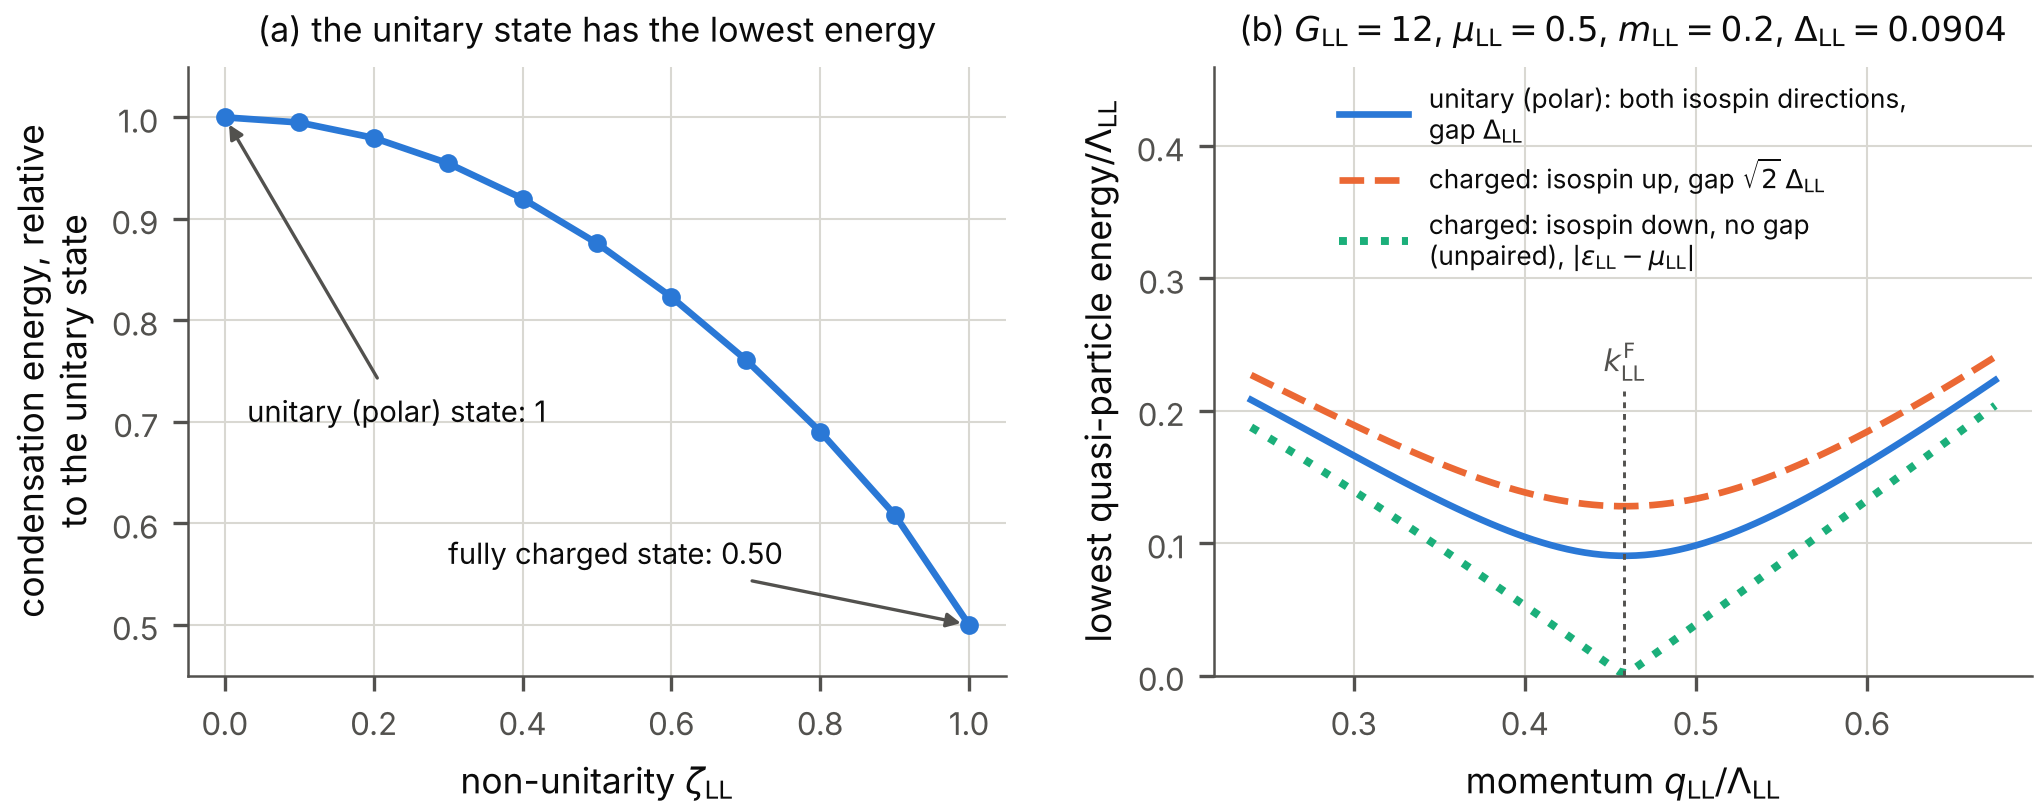
\includegraphics[width=1\textwidth,height=\textheight]{figures/fig_ex_energy.png}

\textbf{Figure 3.} Why the unitary condensate wins (\(G_{\rm LL}=12\),
\(\mu_{\rm LL}=0.5\), \(m_{\rm LL}=0.2\), \(\Lambda_{\rm LL}=1\)). (a)
The minimum of the grand potential at fixed non-unitarity
\(\zeta_{\rm LL}\), divided by the minimum of the unitary condensate:
the condensation energy relative to that of the unitary condensate. It
falls monotonically to exactly one half at \(\zeta_{\rm LL}=1\). (b) The
lowest quasi-particle energies near the Fermi momentum
\(k^{\rm F}_{\rm LL}\) for the same parameters. The unitary (polar)
condensate has the gap \(\Delta_{\rm LL}={}0.090417\) in both isospin
directions (blue, solid). The fully charged condensate with the same
\(\lvert\vec d_{\rm LL}\rvert\) has the gap \(\sqrt2\Delta_{\rm LL}\)
for isospin up (orange, dashed) and no gap for isospin down (green,
dotted): those particles are unpaired. Data:
\texttt{data/sl\_sf\_omega\_zeta.csv} and
\texttt{data/sl\_sf\_dispersion.csv}, written by the command
\texttt{superfluid} of the program \texttt{superloop}; drawn by
\texttt{explanations/code/make\_explain\_figures.py}.

\hypertarget{the-same-physics-in-helium-3}{%
\subsection{7.5 The same physics in helium
3}\label{the-same-physics-in-helium-3}}

In superfluid helium 3 the atoms (fermions) form pairs of spin 1 and
orbital angular momentum 1. The spin part of their gap is a \(2\times2\)
matrix of exactly the form (6.4), with the spin in place of the isospin
and a complex vector of the spin space in place of \(\vec d_{\rm LL}\);
the words ``unitary'' and ``non-unitary'' come from that theory. The two
phases of helium 3 that exist without a magnetic field, the B phase and
the A phase, are unitary. The A₁ phase, which exists only in a magnetic
field and only in a narrow interval of temperature below the transition,
contains only pairs with both spins up: it is non-unitary, the analogue
of the charged condensate of example 6. The magnetic field favors one
spin direction; without it, the unitary phases win, for the reason of
Section 7.4.

\hypertarget{scalar-or-pseudoscalar}{%
\subsection{7.6 Scalar or pseudoscalar}\label{scalar-or-pseudoscalar}}

Both kinds of spin-zero pairs, the scalar (\(0^+\)) and the pseudoscalar
(\(0^-\)) of Eq. (5.2), are isospin triplets. The manuscript compares
them at the same coupling (\(G_{\rm LL}=12\), \(\mu_{\rm LL}=0.5\)): for
\(m_{\rm LL}=0.2\) the minimum of \(\Omega_{\rm LL}\) is
\(-9.720605\times10^{-5}\) in the scalar channel and
\(-4.685258\times10^{-5}\) in the pseudoscalar channel, so the scalar
condensate wins; for \(m_{\rm LL}=0\) both are
\(-1.384064\times10^{-4}\), because a chiral rotation of the field maps
one channel onto the other. For massive spinor charges the ground state
is therefore the \textbf{scalar, unitary, isospin-triplet condensate}.

\hypertarget{electrically-neutral}{%
\section{8. ``Electrically neutral''}\label{electrically-neutral}}

\hypertarget{neutral-pairs}{%
\subsection{8.1 Neutral pairs}\label{neutral-pairs}}

By Eq. (7.4), the pairs of every unitary condensate have the average
charge 0. In the polar condensate along the third axis,
\(\vec d_{\rm LL}\propto(0,0,1)\), which the manuscript names as the
ground state, more is true: every single pair consists of one up and one
down particle and has the charge exactly 0, not only on average (example
1 of Section 7.3).

\hypertarget{the-symmetry-that-survives-the-condensation}{%
\subsection{8.2 The symmetry that survives the
condensation}\label{the-symmetry-that-survives-the-condensation}}

Four generators act on the order parameter: the three isospin generators
\(T^\iota_{\rm LL}\) and the fermion number \(F_{\rm LL}\) (the group
\(SU(2)_{\rm v}\times U(1)^{\rm F}_{\rm LL}\)). Their action follows
from their action on the field: under the symmetry generated by
\(T^\iota_{\rm LL}\) the field changes by
\(\tfrac12\tau^{\rm LL}_\iota\) on the isospin index, under
\(F_{\rm LL}\) by the unit matrix; the pair operators (6.2) change
accordingly, and so does their expectation value \(\vec d_{\rm LL}\).
The program derives the result from the pair matrices (check X-7):
\(T^\iota_{\rm LL}\) rotates the vector \(\vec d_{\rm LL}\) about the
axis \(\iota\), and \(F_{\rm LL}\) multiplies it by \(2i\). A generator
is \textbf{unbroken} if it leaves \(\vec d_{\rm LL}\) unchanged; then
the transformation it generates leaves the condensate unchanged. A
generator is \textbf{broken} if it changes \(\vec d_{\rm LL}\); then it
maps the condensate onto a different condensate of the same grand
potential.

\begin{itemize}
\tightlist
\item
  \emph{Unitary condensates},
  \(\vec d_{\rm LL}=e^{i\theta_{\rm LL}}\lvert\vec d_{\rm LL}\rvert\)
  times a real unit vector. A rotation of \(\vec d_{\rm LL}\) leaves it
  unchanged only if its axis is that real vector; a multiplication by a
  phase never does. Exactly one generator is unbroken: the isospin
  rotation about the real direction of \(\vec d_{\rm LL}\), the
  generator
  \(e^{-i\theta_{\rm LL}}\sum_\iota d^\iota_{\rm LL}T^\iota_{\rm LL}/\lvert\vec d_{\rm LL}\rvert\);
  three of the four generators are broken. \textbf{For the polar
  condensate along the third axis the unbroken generator is
  \(T^3_{\rm LL}=Q_{\rm LL}\): the electric charge remains a conserved
  quantity in the condensate.} This is the precise meaning of
  ``electrically neutral'' in the manuscript.
\item
  \emph{The charged condensate with up-up pairs.} Its only unbroken
  generator is \(\tfrac12F_{\rm LL}-T^3_{\rm LL}\), which is 0 on an up
  particle and 1 on a down particle: the \textbf{number of down
  particles}, which is conserved because the down particles are not
  paired. The electric charge and the fermion number are both broken:
  this condensate has no definite electric charge, being a condensate of
  pairs of the charge \(+1\). (For the down-down condensate the unbroken
  generator is \(\tfrac12F_{\rm LL}+T^3_{\rm LL}\), the number of up
  particles.)
\item
  \emph{The partly non-unitary condensate} breaks all four generators.
\end{itemize}

These results are the column ``unbroken generator'' of the table of
Section 7.3.

\hypertarget{what-neutrality-means-physically}{%
\subsection{8.3 What neutrality means
physically}\label{what-neutrality-means-physically}}

If the electric charge \(Q_{\rm LL}\) were coupled to an electromagnetic
field (the model of the manuscript contains none), a condensate of
charged pairs would be a \textbf{superconductor}: inside it the photon
would acquire a mass, and magnetic fields would be expelled (the
Meissner effect). This is what the electrons of a metal do: their pairs
have the charge of two electrons. A condensate of neutral pairs leaves
the electric charge unbroken: the photon stays massless, magnetic fields
are not expelled, and the condensate is a \textbf{superfluid}, like
helium 4, helium 3, and the neutron superfluid of neutron stars. (The
neutron-neutron pairs are isospin triplets with the isospin projection
\(-1\), but they are electrically neutral, because for nucleons the
charge is the isospin projection plus half the baryon number.)
``Electrically neutral'' thus says: \textbf{the spin-zero condensate of
the spinor charges is a superfluid, not a superconductor.}

\hypertarget{how-precise-the-word-neutral-is}{%
\subsection{8.4 How precise the word ``neutral''
is}\label{how-precise-the-word-neutral-is}}

The model of the manuscript is exactly invariant under isospin
rotations, and an isospin rotation maps one ground state onto another of
the same grand potential. The unitary condensates therefore form a
family: \(e^{i\theta_{\rm LL}}\lvert\vec d_{\rm LL}\rvert\) times any
real unit vector, all with the same grand potential. For each of them
the average charge of a pair is 0 (Eq. (7.4)). Only for the direction of
the third axis is every pair neutral and the electric charge
\(T^3_{\rm LL}\) unbroken; for another direction the unbroken generator
is the isospin component along that direction, and the pairs are
superpositions of the charges \(+1\), 0 and \(-1\) with the average 0
(examples 2 to 4 of Section 7.3). The manuscript names the polar
condensate along the third axis ``up to an isospin rotation'': the
representative of the family that keeps the electric charge exact.

Which direction a real system would choose is decided by interactions
that distinguish the third isospin axis, which the model does not
contain; the coupling of the electric charge to a photon would be one. A
simple illustration: if the coupling in the channel of charge 0 (the
pair operator \(\Pi^3_{\rm LL}\)) were slightly larger than in the other
two channels, the quadratic term of the grand potential would favor the
third axis; if it were slightly smaller, it would favor a real direction
in the plane of the first two axes. In both cases the minimum is a
unitary condensate (Section 7.4), and in both cases the average charge
of its pairs is zero.

\hypertarget{the-pair-that-is-a-singlet-of-the-whole-super-loop-requires-two-species}{%
\section{9. ``The pair that is a singlet of the whole super-loop
requires two
species''}\label{the-pair-that-is-a-singlet-of-the-whole-super-loop-requires-two-species}}

\hypertarget{what-a-singlet-of-the-whole-super-loop-is}{%
\subsection{9.1 What a singlet of the whole super-loop
is}\label{what-a-singlet-of-the-whole-super-loop-is}}

A \textbf{singlet of the whole super-loop} is a pair that every symmetry
(2.4) leaves unchanged: it has spin 0 (unchanged by the Lorentz
transformations \(\mathbf g\)) \textbf{and} isospin 0 (unchanged by the
isospin rotations \(\mathbf v\)), and hence the electric charge 0. The
isospin-triplet pairs of Sections 5 to 8 are Lorentz scalars but not
isospin singlets. Among the pairs of two spinor charges there is exactly
one candidate: spin \(\tfrac12\) times spin \(\tfrac12\) gives spin 0
and spin 1, isospin \(\tfrac12\) times isospin \(\tfrac12\) gives
isospin 0 and isospin 1, and the combination with spin 0 and isospin 0
occurs once.

\hypertarget{the-super-loops-own-pair-the-product-of-two-spinor-charges}{%
\subsection{9.2 The super-loop's own pair: the product of two spinor
charges}\label{the-super-loops-own-pair-the-product-of-two-spinor-charges}}

The super-loop multiplies two spinor charges. By Eq. (2.1) with
\(\mathbf a=\mathbf c=0\),
\[(\mathbf b\,\mathbf e_4)(\mathbf b'\mathbf e_4)=-\bar{\mathbf b}'\mathbf b , \tag{9.1}\]
a bi-quaternion. Examples: \(\mathbf e_4\mathbf e_4=-\mathbf e_0\),
\(\mathbf e_4\mathbf e_5=\mathbf e_1\),
\(\mathbf e_5\mathbf e_4=-\mathbf e_1\) (check X-8). A bi-quaternion has
a \textbf{scalar part} (the coefficient of \(\mathbf e_0\)) and an
\textbf{imaginary part} (the coefficients of
\(\mathbf e_1,\mathbf e_2,\mathbf e_3\)). The scalar part of
\(\bar{\mathbf b}'\mathbf b\) is \(N_{\rm LL}(\mathbf b',\mathbf b)\):
in the product of two quaternion units, the conjugate of a unit times
the same unit is 1, and the conjugate of a unit times a different unit
is imaginary. Hence
\[\text{scalar part of }(\mathbf b\,\mathbf e_4)(\mathbf b'\mathbf e_4)=-N_{\rm LL}(\mathbf b',\mathbf b). \tag{9.2}\]

\hypertarget{the-scalar-part-is-the-singlet}{%
\subsection{9.3 The scalar part is the
singlet}\label{the-scalar-part-is-the-singlet}}

Under a symmetry (2.4),
\(\mathbf b\mapsto\mathbf v\mathbf b\bar{\mathbf g}\) and
\(\mathbf b'\mapsto\mathbf v\mathbf b'\bar{\mathbf g}\). Because the
norm of bi-quaternions is multiplicative, so is its polarization:
\(N_{\rm LL}(\mathbf v\mathbf b'\bar{\mathbf g},\mathbf v\mathbf b\bar{\mathbf g})=N_{\rm LL}(\mathbf v)\,N_{\rm LL}(\mathbf g)\,N_{\rm LL}(\mathbf b',\mathbf b)=N_{\rm LL}(\mathbf b',\mathbf b)\).
(Expand
\(N_{\rm LL}(\mathbf v(\mathbf b+\mathbf b'))=N_{\rm LL}(\mathbf v)N_{\rm LL}(\mathbf b+\mathbf b')\)
in the two arguments and compare the mixed terms.) \textbf{The scalar
part is unchanged by every symmetry of the super-loop: it is the
singlet} --- spin 0, isospin 0, charge 0. In the matrix form of Section
2.2 it is
\[N_{\rm LL}(\mathbf b',\mathbf b)=\tfrac12\,\mathrm{tr}\big(M_{\rm LL}(\mathbf b)^T\,\mathsf E_{\rm LL}\,M_{\rm LL}(\mathbf b')\,\mathsf E_{\rm LL}^T\big): \tag{9.3}\]
the first \(\mathsf E_{\rm LL}\) joins the two isospin indices (the rows
of the two matrices) into the isospin singlet, the second joins the two
spinor indices (the columns) into the spin singlet. (The imaginary part
of Eq. (9.1) is unchanged by the isospin rotations and turns under the
Lorentz transformations like a Lorentz generator: a pair of spin 1 and
isospin 0.) The program verifies Eq. (9.3) and the invariance on 200
random pairs of bi-quaternions (check X-8).

\hypertarget{the-singlet-is-symmetric-so-one-field-has-no-such-pair}{%
\subsection{9.4 The singlet is symmetric, so one field has no such
pair}\label{the-singlet-is-symmetric-so-one-field-has-no-such-pair}}

\(N_{\rm LL}(\mathbf b',\mathbf b)=N_{\rm LL}(\mathbf b,\mathbf b')\):
the singlet is \textbf{symmetric} in the two spinor charges. In the
matrix form (9.3) this is the rule of signs again: two antisymmetric
factors \(\mathsf E_{\rm LL}\), \((-1)(-1)=+1\). Now let the
coefficients of \(\mathbf b\) be the anticommuting components of one
fermion field, as the particles of Section 2.4 require. Then the pair of
the field with itself is
\[N_{\rm LL}(\mathbf b,\mathbf b)=\sum_{p=0}^3\xi^{\rm LL}_p(\mathbf b)\,\xi^{\rm LL}_p(\mathbf b)=0 ,\]
because the square of every anticommuting component is zero. In the
language of Section 5: the isospin-singlet pair matrix
\(C_{\rm LL}\gamma^{\rm ch}_{\rm LL}\otimes\mathsf E_{\rm LL}\) has the
sign \((-1)(-1)=+1\) and vanishes identically (check X-2). \textbf{One
kind of fermion field has no pair that is a singlet of the whole
super-loop.} (The imaginary part of Eq. (9.1), by contrast, is
antisymmetric in the two spinor charges (check X-8), so it survives for
one field: a pair of spin 1 and isospin 0, the channel of the deuteron
in the nucleon analogy of Section 3.4.)

\hypertarget{two-species}{%
\subsection{9.5 Two species}\label{two-species}}

Now take two copies of the field, \(\Psi^{(1)}_{\rm LL}\) and
\(\Psi^{(2)}_{\rm LL}\), two \textbf{species}, combined into one field
of 16 components with a species index of two values. A pair matrix then
has a third factor, on the species index. The singlet of the whole
super-loop becomes
\[\mathsf K^{\rm s}_{\rm LL}=C_{\rm LL}\gamma^{\rm ch}_{\rm LL}\otimes\mathsf E_{\rm LL}\otimes\mathsf E_{\rm LL} \tag{9.4}\]
(Dirac \(\otimes\) isospin \(\otimes\) species). The species factor
\(\mathsf E_{\rm LL}\) joins a particle of species 1 with a particle of
species 2, antisymmetrically,
\((\lvert12\rangle-\lvert21\rangle)/\sqrt2\): a \textbf{species
singlet}. The signs are \((-1)(-1)(-1)=-1\): the matrix is
antisymmetric, as fermions require, and it keeps 8 terms (check X-9).
The missing minus sign is supplied by the species. In the language of
bi-quaternions: \(N_{\rm LL}(\mathbf b^{(2)},\mathbf b^{(1)})\) with the
components of two different fields is not zero, and it changes sign when
the two species are exchanged.

The condensate of this pair is fully gapped: all sixteen positive
eigenvalues of its Bogoliubov-de Gennes matrix are \(E^-_{\rm LL}\)
(eight times) and \(E^+_{\rm LL}\) (eight times) of Eq. (6.5). At the
test point of the program \texttt{superloop} (momentum
\((0.13,-0.21,0.07)\), \(m_{\rm LL}=0.2\), \(\mu_{\rm LL}=0.5\), gap
0.3) they are \(E^-_{\rm LL}={}0.347098\) and
\(E^+_{\rm LL}={}0.878250\). It breaks only the fermion number and keeps
the isospin, the electric charge and the Lorentz invariance. This is the
superfluid of spin-zero pairs that are singlets in the strict sense:
singlets of the whole super-loop.

The other pairs of two species follow from the same rule of signs (table
of Section 5.3, Figure 1): the isospin triplet with each species paired
with itself (\(\sigma^{\rm LL}_0\) on the species index, signs
\((-1)(+1)(+1)=-1\)) survives --- each species forms its own triplet
condensate; the isospin triplet in the species singlet
(\((-1)(+1)(-1)=+1\)) and the isospin singlet with each species paired
with itself (\((-1)(-1)(+1)=+1\)) vanish.

\hypertarget{a-second-label-that-carries-the-antisymmetry-examples}{%
\subsection{9.6 A second label that carries the antisymmetry:
examples}\label{a-second-label-that-carries-the-antisymmetry-examples}}

\begin{itemize}
\tightlist
\item
  \emph{Helium.} Two electrons in the same orbital can only form the
  spin singlet; in two different orbitals (the configuration 1s2s) the
  spatial part can be antisymmetric and the spin triplet becomes
  possible (Section 3.4). The orbital label plays the role of the
  species label.
\item
  \emph{Nucleons.} Two nucleons in an s-wave cannot have spin 0 and
  isospin 0 (Section 3.4). A pair with these quantum numbers needs a
  second, distinguishable kind of particle.
\item
  \emph{Dense quark matter.} Quarks carry a Dirac index, a color index
  with three values and a flavor index. The most attractive pairs of
  quarks have spin zero (the same antisymmetric Dirac factor as here)
  and are antisymmetric in color (the color ``antitriplet''). The rule
  of signs then requires an antisymmetric flavor factor: the flavor
  singlet of two flavors, the up and the down quark. Matter of a single
  flavor of quarks cannot form this pair; it pairs with spin 1 instead.
  This is the same bookkeeping as for the spinor charges, with color and
  flavor in place of isospin and species.
\end{itemize}

\hypertarget{the-sentence-again-in-one-table}{%
\section{10. The sentence again, in one
table}\label{the-sentence-again-in-one-table}}

\sptkeptpenalty=10000
\begin{longtable}[]{@{}
  >{\raggedright\arraybackslash}p{(\columnwidth - 6\tabcolsep) * \real{0.1379}}
  >{\raggedright\arraybackslash}p{(\columnwidth - 6\tabcolsep) * \real{0.3333}}
  >{\raggedright\arraybackslash}p{(\columnwidth - 6\tabcolsep) * \real{0.3103}}
  >{\raggedright\arraybackslash}p{(\columnwidth - 6\tabcolsep) * \real{0.2184}}@{}}
\toprule\noalign{}
\begin{minipage}[b]{\linewidth}\raggedright
part of the sentence
\end{minipage} & \begin{minipage}[b]{\linewidth}\raggedright
precise meaning
\end{minipage} & \begin{minipage}[b]{\linewidth}\raggedright
why
\end{minipage} & \begin{minipage}[b]{\linewidth}\raggedright
where it is computed
\end{minipage} \\
\midrule\noalign{}
\endhead
\bottomrule\noalign{}
\endlastfoot
``the spin-zero superfluid'' & a condensate of pairs whose Dirac factor
is \(C_{\rm LL}\gamma^{\rm ch}_{\rm LL}\) (scalar, \(0^+\)); the fermion
number is broken & the attractive contact interaction acts in the
spin-zero s-wave channels; the scalar channel wins for massive spinor
charges & checks X-3; Section 7.6 \\*
``of its spinor charges'' & the particles are the quanta of the Dirac
isodoublet \(\Psi_{\rm LL}\) built from the spinor charges
\(\mathbf b\,\mathbf e_4\): fermions with the charges \(\pm\tfrac12\) &
spinor number \(-1\) and the spin-statistics theorem & Section 2; check
X-8 \\*
``condenses'' & the minimum of \(\Omega_{\rm LL}\) lies at
\(\vec d_{\rm LL}\neq0\) & gap equation (6.7); with a Fermi sea every
attraction suffices & gap \(0.090417\), \(\Omega_{\rm LL}\)
\(-9.720605\times10^{-5}\) \\*
``in an isospin-triplet \ldots{} state'' & the isospin factor of every
spin-zero pair matrix is symmetric: isospin 1, pairs of charge \(+1\),
0, \(-1\) & rule of Pauli: antisymmetric Dirac factor, so symmetric
isospin factor & checks X-1 to X-4, X-10 \\*
``unitary'' & \(\zeta_{\rm LL}=0\):
\(\mathsf D_{\rm LL}\mathsf D_{\rm LL}^\dagger=\lvert\vec d_{\rm LL}\rvert^2\sigma^{\rm LL}_0\);
one gap for both isospin directions; average isospin of a pair 0 &
concavity of \(E^+_{\rm LL}+E^-_{\rm LL}\) in the squared gap (Jensen);
the fully non-unitary state has half the condensation energy & checks
X-5, X-6; ratio \(0.500000\) \\*
``electrically neutral'' & the average charge of a pair is 0 in every
unitary state; for \(\vec d_{\rm LL}\propto(0,0,1)\) every pair has the
charge 0 and \(Q_{\rm LL}=T^3_{\rm LL}\) is unbroken: a superfluid, not
a superconductor & Eq. (7.4); the unbroken generator of a unitary state
is the isospin rotation about its real direction & checks X-5, X-7 \\*
``the pair that is a singlet of the whole super-loop requires two
species'' & the scalar part \(-N_{\rm LL}(\mathbf b',\mathbf b)\) of the
product of two spinor charges (spin 0, isospin 0, charge 0) is symmetric
in the two spinor charges, so it vanishes for one fermion field; with
two species it is \(\mathsf K^{\rm s}_{\rm LL}\), antisymmetric &
antisymmetric times antisymmetric is symmetric; the species singlet
supplies the missing sign & checks X-8 to X-10; energies \(0.347098\),
\(0.878250\) \\
\end{longtable}

\hypertarget{provenance-programs-commands-reports-data-figures}{%
\section{11. Provenance: programs, commands, reports, data,
figures}\label{provenance-programs-commands-reports-data-figures}}

\hypertarget{how-to-reproduce-everything}{%
\subsection{11.1 How to reproduce
everything}\label{how-to-reproduce-everything}}

From the folder Revision\_SuperLoop of the repository:

\begin{verbatim}
# 1. the numbers of the superfluid (data/sl_sf_*.csv) and the report data/sl_superfluid_checks.txt
cargo run --release --manifest-path code/superloop-rs/Cargo.toml -- superfluid
# 2. the examples of this document (explanations/data/ex_*) and the checks X-1 to X-10
(cd explanations && cargo run --release --manifest-path code/explain-rs/Cargo.toml)
# 3. the three figures (explanations/figures/fig_ex_*.pdf and .png)
python3 explanations/code/make_explain_figures.py
# 4. everything of the folder, all checks and all documents, with one verdict ("ALL PASS")
bash code/scripts/check_all.sh
\end{verbatim}

Requirements: a Rust toolchain for the edition 2021; Python 3 with NumPy
and Matplotlib; for the documents pandoc, XeLaTeX and latexmk, the
DejaVu fonts and the Latin Modern Math font. The two Rust programs use
the library crate \texttt{code/spacetimes-rs} of the repository (complex
numbers, Hermitian diagonalization, the writer of data files); no crate
is downloaded.

\hypertarget{the-program-of-the-examples}{%
\subsection{11.2 The program of the
examples}\label{the-program-of-the-examples}}

\texttt{explanations/code/explain-rs/src/main.rs} (977 lines of
commented Rust, binary \texttt{explain\_superfluid}) builds the Pauli
matrices, \(\mathsf E_{\rm LL}\), the chiral Dirac matrices,
\(C_{\rm LL}\) and \(\gamma^{\rm ch}_{\rm LL}\), the generators of the
Lorentz group and of isospin on the field, all pair matrices of Sections
4, 5 and 9, the seven example order parameters, and the bi-quaternions
with their Cayley-Dickson product, and checks every statement of this
document about them:

\begin{itemize}
\tightlist
\item
  X-1: the exchange signs of the Dirac, isospin and species factors and
  the rule that the sign of a Kronecker product is the product of the
  signs (24 products);
\item
  X-2: only the antisymmetric part of a pair matrix survives; the number
  of surviving terms of every spin-zero pair of one field (4 for each
  triplet, 0 for each singlet);
\item
  X-3: Lorentz invariance of the eight spin-zero pair matrices, and
  their isospin from the Casimir operator (2 for the triplet, 0 for the
  singlet);
\item
  X-4: the electric charges \(+1\), 0, \(-1\) of the triplet pairs (and
  0 for the vanishing singlet);
\item
  X-5: the pair wavefunction \(\mathsf D_{\rm LL}\), the fractions
  (7.3), the average charge (7.4) and the average isospin (7.5) of seven
  examples and 200 random order parameters;
\item
  X-6: the two gaps (7.2) and the unpaired isospin direction of the
  charged states;
\item
  X-7: the action of the four generators on \(\vec d_{\rm LL}\), derived
  from the pair matrices, and the unbroken generators of the examples;
\item
  X-8: the matrix of a bi-quaternion, the non-associativity, the
  multiplicative norm, the automorphisms (2.4), the product of two
  spinor charges (9.1), the singlet (9.3), its symmetry and its
  invariance (200 random pairs);
\item
  X-9: the pairs of two species, among them the singlet of the whole
  super-loop \(\mathsf K^{\rm s}_{\rm LL}\);
\item
  X-10: the counting of the two-particle states of Section 3.4, by the
  traces of projectors on the total spin, the total isospin, the total
  species spin and the exchange symmetry.
\end{itemize}

Every equality is tested with the tolerance \(10^{-12}\) (every matrix
entry is \(0\), \(\pm1\), \(\pm i\), \(\pm\tfrac12\) or a small
integer); random numbers come from a fixed seed, so every run gives the
same output. The report of the program, verbatim
(\texttt{explanations/data/ex\_superfluid\_checks.txt}):

\begin{verbatim}
Revision_SuperLoop, folder explanations, program `explain_superfluid`: the examples of the explanation of the sentence on the spin-zero superfluid of the spinor charges
10 of 10 checks passed

[PASS] X-1  exchange signs: the Dirac factors C_LL gamma_ch (0+) and C_LL (0-) of the spin-zero pairs are antisymmetric (in each chirality block they are eps2, the spin singlet up-down minus down-up), the isospin factors eps2 tau_1, eps2 tau_2, eps2 tau_3 are symmetric (isospin 1) and eps2 is antisymmetric (isospin 0), the species factors eps2 (antisymmetric) and sigma_0 (symmetric); gamma_ch = diag(-1,-1,1,1), C_LL = diag(eps2, -eps2), C_LL gamma_ch = -diag(eps2, eps2); and the exchange sign of each of the 24 Kronecker products of a Dirac, an isospin and possibly a species factor is the product of the signs of its factors  -- signs: Dirac [-1, -1], isospin [1, 1, 1, -1], species [-1, 1]
[PASS] X-2  the Pauli principle in numbers: for anticommuting components the pair Psi_LL^T Kch Psi_LL keeps only the antisymmetric part (Kch - Kch^T)/2 of its matrix; counting the products of two different components with a non-zero coefficient, each of the six isospin-triplet matrices (C_LL gamma_ch or C_LL times eps2 tau_iota) gives 4 terms, and each of the two isospin-singlet matrices (C_LL gamma_ch or C_LL times eps2) gives 0: the spin-zero isospin-singlet pair of one field vanishes identically  -- terms (C_LL gamma_ch with eps2 tau_1, eps2 tau_2, eps2 tau_3, eps2; then C_LL with the same): [4, 4, 4, 0, 4, 4, 4, 0]
[PASS] X-3  the eight spin-zero matrices are Lorentz invariant (generator^T Kch + Kch generator = 0 for the three rotations and the three boosts of Psi_LL), and the isospin Casimir sum_iota of the twofold change under T_LL^iota is 2 Kch = 1(1+1) Kch for the six matrices with eps2 tau_iota (isospin 1, triplet) and 0 for the two matrices with eps2 (isospin 0, singlet)
[PASS] X-4  electric charges of the pairs: the pair operator Psi_LL^T Kch Psi_LL annihilates two particles of total charge Q_LL(Kch), the number with generator^T Kch + Kch generator = Q_LL(Kch) Kch for the generator T_LL^3 = Q_LL: Kch_1 - i Kch_2 (isospin part [[2,0],[0,0]], up with up) has Q_LL(Kch) = +1, Kch_3 (isospin part [[0,-1],[-1,0]], up with down, symmetric) has 0, Kch_1 + i Kch_2 (isospin part [[0,0],[0,-2]], down with down) has -1, and the vanishing singlet C_LL gamma_ch (x) eps2 (up with down, antisymmetric) has 0  -- Q_LL(Kch) = +1, 0, -1, 0
[PASS] X-5  the pairs of seven example condensates (|dvec| = 1) and of 200 random ones: the condensed pairs have the isospin wavefunction -sum_iota d_iota tau_iota eps2 (= sum_iota d_iota eps2 tau_iota^*), which is the isospin part Dpair = sum_iota d_iota (eps2 tau_iota)^dag of the pairing block of the Bogoliubov-de Gennes matrix; the weights of its entries up-up, up-down, down-down are the fractions of pairs with the charges +1, 0, -1; the average charge of a pair, fraction(+1) - fraction(-1), equals the third component of i cross(dvec, dvec^*)/|dvec|^2, the whole vector is the average isospin of a pair, and its length is zeta: unitary states (zeta = 0) have pairs of average charge 0 and average isospin 0, the charged states (zeta = 1) consist of pairs of charge +1 only or -1 only  -- polar along the third axis: charges +1/0/-1 0/1/0, average charge 0, zeta 0; polar along the first axis: charges +1/0/-1 0.5/0/0.5, average charge 0, zeta 0; polar along (1,2,2)/3: charges +1/0/-1 0.277778/0.444444/0.277778, average charge 0, zeta 0; unitary with a phase: charges +1/0/-1 0.18/0.64/0.18, average charge 0, zeta 0; partly non-unitary: charges +1/0/-1 0.9/0/0.1, average charge 0.8, zeta 0.8; charged, up-up pairs: charges +1/0/-1 1/0/0, average charge 1, zeta 1; charged, down-down pairs: charges +1/0/-1 0/0/1, average charge -1, zeta 1
[PASS] X-6  gaps of the examples and of 200 random dvec: the eigenvalues of the 2 x 2 gap matrix times its Hermitian conjugate are |dvec|^2 (1 - zeta) and |dvec|^2 (1 + zeta), so unitary states have the single gap Delta_+ = Delta_- = |dvec| for both isospin directions, and the charged states have Delta_+ = sqrt2 |dvec| and Delta_- = 0, the gapless direction being isospin down for the up-up state and isospin up for the down-down state (those particles are not paired)  -- polar along the third axis: Delta_+ 1, Delta_- 1; polar along the first axis: Delta_+ 1, Delta_- 1; polar along (1,2,2)/3: Delta_+ 1, Delta_- 1; unitary with a phase: Delta_+ 1, Delta_- 1; partly non-unitary: Delta_+ 1.341641, Delta_- 0.447214; charged, up-up pairs: Delta_+ 1.414214, Delta_- 0 (unpaired: down); charged, down-down pairs: Delta_+ 1.414214, Delta_- 0 (unpaired: up)
[PASS] X-7  unbroken generators of SU(2)_v x U(1)_F_LL: the action of each generator on dvec is derived from its action on the pair matrices (generator^T Kch_iota + Kch_iota generator is again a combination of Kch_1, Kch_2, Kch_3; true for all 12 cases), and it is: T_LL^iota changes dvec by minus the cross product of the unit vector iota with dvec (a rotation of dvec about the axis iota), F_LL multiplies dvec by 2 i (20 random dvec); a generator is unbroken if it leaves dvec unchanged; for every unitary example exactly one generator is unbroken, the isospin rotation about the real direction of dvec (for the polar state along the third axis that is T_LL^3 = Q_LL: the electric charge is unbroken); for the charged state with up-up pairs the only unbroken generator is F_LL/2 - T_LL^3, the number of isospin-down particles (they are not paired), and for the down-down state F_LL/2 + T_LL^3; the partly non-unitary state breaks all four generators  -- polar along the third axis: isospin rotation about the axis (0, 0, 1): T_LL^3 = Q_LL; polar along the first axis: isospin rotation about the axis (1, 0, 0); polar along (1,2,2)/3: isospin rotation about the axis (0.333333, 0.666667, 0.666667); unitary with a phase: isospin rotation about the axis (0, 0.6, 0.8); partly non-unitary: none; charged, up-up pairs: F_LL/2 - T_LL^3, the number of isospin-down particles; charged, down-down pairs: F_LL/2 + T_LL^3, the number of isospin-up particles
[PASS] X-8  the singlet of the whole super-loop (200 random pairs of bi-quaternions bS, bS' with Gaussian-integer coefficients): M_LL is multiplicative and det M_LL(bS) = N_LL(bS); N_LL(bS', bS) = (1/2) tr(M_LL(bS)^T eps2 M_LL(bS') eps2^T), a contraction of the two isospin indices with eps2 (isospin 0) and of the two spinor indices with eps2 (spin 0); it is the scalar part of bS'bar bS and minus the scalar part of the bi-octonion product (bS e4)(bS' e4) (Cayley-Dickson product), which is SYMMETRIC under the exchange of the two spinor charges, while the imaginary part is antisymmetric; it is invariant under bS -> vI bS gLbar (vI = e3, gL = 1 + i e1 + e2, and random complex unit gL); examples: e4 e4 = -e0, e4 e5 = e1, e5 e4 = -e1; the product of B_LL is not associative ((e1 e2) e4 = e7 but e1 (e2 e4) = -e7), its norm is multiplicative (N_LL(x y) = N_LL(x) N_LL(y) for 200 random pairs of bi-octonions, so the unit bi-octonions are closed under the product), and varphi_(gL,vI) preserves the product (the same 200 pairs; vI = e3 and vI = (e0 + e1 + e2 + e3)/2)  -- determinant and contraction true, Cayley-Dickson product true, exchange symmetry true, examples true, non-associativity true, multiplicative norm true, automorphism true
[PASS] X-9  two species: the super-loop singlet Kch_singlet = C_LL gamma_ch (x) eps2 (x) eps2 (spin 0, isospin 0, species singlet: species Casimir 0) is antisymmetric (signs -1, -1, -1), Lorentz invariant, of charge 0, and keeps 8 terms; the same Dirac and isospin factors with the species factor sigma_0 (each species paired with itself) give a symmetric matrix and 0 terms, as for one field; the isospin triplet eps2 tau_3 with sigma_0 keeps 8 terms (each species pairs as a triplet) and with the species singlet eps2 vanishes
[PASS] X-10  the nucleon analogy (two particles of spin 1/2 and isospin 1/2 in a relative s-wave, which is symmetric under the exchange of the positions, so that the spin-isospin part must be antisymmetric): of the 16 spin-isospin states the antisymmetric ones are the 3 states of spin 0 and isospin 1 and the 3 states of spin 1 and isospin 0; spin 0 with isospin 0 (1 state) and spin 1 with isospin 1 (9 states) are symmetric and forbidden; with two species (64 states) the state of spin 0, isospin 0 and species singlet is antisymmetric and allowed (counted by the traces of the projectors on total spin, total isospin, total species spin and exchange symmetry)  -- one kind: [(0, 0, 0), (0, 1, 3), (1, 0, 3), (1, 1, 0)]; two species: [(0, 0, 0, 1), (0, 0, 1, 0), (0, 1, 0, 0), (0, 1, 1, 9), (1, 0, 0, 0), (1, 0, 1, 9), (1, 1, 0, 9), (1, 1, 1, 0)]
\end{verbatim}

\hypertarget{the-data-files-of-the-examples}{%
\subsection{11.3 The data files of the
examples}\label{the-data-files-of-the-examples}}

\sptkeptpenalty=10000
\begin{longtable}[]{@{}
  >{\raggedright\arraybackslash}p{(\columnwidth - 4\tabcolsep) * \real{0.1429}}
  >{\raggedright\arraybackslash}p{(\columnwidth - 4\tabcolsep) * \real{0.4286}}
  >{\raggedright\arraybackslash}p{(\columnwidth - 4\tabcolsep) * \real{0.4286}}@{}}
\toprule\noalign{}
\begin{minipage}[b]{\linewidth}\raggedright
file
\end{minipage} & \begin{minipage}[b]{\linewidth}\raggedright
content
\end{minipage} & \begin{minipage}[b]{\linewidth}\raggedright
columns
\end{minipage} \\
\midrule\noalign{}
\endhead
\bottomrule\noalign{}
\endlastfoot
\texttt{explanations/data/ex\_pair\_matrices.csv} & the spin-zero pair
matrices of one field and of two species (table of Section 5.3) &
\texttt{pair\_matrix}, \texttt{spin\_parity}, \texttt{isospin},
\texttt{species}, \texttt{exchange\_sign\_Dirac},
\texttt{exchange\_sign\_isospin}, \texttt{exchange\_sign\_species},
\texttt{exchange\_sign\_total}, \texttt{nonzero\_pair\_terms},
\texttt{pair\_charge} \\*
\texttt{explanations/data/ex\_states.csv} & the seven example
condensates (table of Section 7.3) & \texttt{state},
\texttt{dvec\_definition}, \texttt{dvec}, \texttt{pairs\_charge\_plus1},
\texttt{pairs\_charge\_0}, \texttt{pairs\_charge\_minus1},
\texttt{average\_pair\_charge}, \texttt{average\_pair\_isospin},
\texttt{zeta}, \texttt{Delta\_+}, \texttt{Delta\_-}, \texttt{unpaired},
\texttt{stabilizer\_dim}, \texttt{unbroken\_generator} \\*
\texttt{explanations/data/ex\_two\_particle\_counting.csv} & the
two-particle states of Section 3.4 & \texttt{total\_spin},
\texttt{total\_isospin}, \texttt{species\_pair},
\texttt{number\_of\_states}, \texttt{antisymmetric\_states},
\texttt{symmetric\_states}, \texttt{allowed\_in\_s\_wave} \\*
\texttt{explanations/data/ex\_superfluid\_checks.txt} & the report of
the checks X-1 to X-10 (Section 11.2) & --- \\
\end{longtable}

Each data file begins with lines starting with \texttt{\#} that name the
program that wrote it and state its content. The plain-text names in the
files are those of the table of symbols (Section 13): \texttt{dvec} is
\(\vec d_{\rm LL}\), \texttt{zeta} is \(\zeta_{\rm LL}\),
\texttt{Delta\_+} and \texttt{Delta\_-} are \(\Delta^+_{\rm LL}\) and
\(\Delta^-_{\rm LL}\), \texttt{eps2} is \(\mathsf E_{\rm LL}\),
\texttt{C\_LL\ gamma\_ch} is \(C_{\rm LL}\gamma^{\rm ch}_{\rm LL}\),
\texttt{(x)} is \(\otimes\), \texttt{Kch\_singlet} is
\(\mathsf K^{\rm s}_{\rm LL}\), \texttt{Dpair} is
\(\mathsf D_{\rm LL}\).

\hypertarget{the-numbers-taken-from-the-program-superloop}{%
\subsection{\texorpdfstring{11.4 The numbers taken from the program
\texttt{superloop}}{11.4 The numbers taken from the program superloop}}\label{the-numbers-taken-from-the-program-superloop}}

The critical couplings, the slope of Bardeen, Cooper and Schrieffer, the
gap at \(G_{\rm LL}=12\), the minima of \(\Omega_{\rm LL}\) and the
energies of the two-species singlet are computed by the command
\texttt{superfluid} of the program \texttt{superloop}
(\texttt{code/superloop-rs}, file \texttt{src/superfluid.rs}). The data
of Figure 3 are its files \texttt{data/sl\_sf\_omega\_zeta.csv} (the
minimum of \(\Omega_{\rm LL}\) at fixed \(\zeta_{\rm LL}\)) and
\texttt{data/sl\_sf\_dispersion.csv} (the quasi-particle energies); the
gaps versus the coupling are in
\texttt{data/sl\_sf\_gap\_vs\_coupling.csv}. The test point of the
two-species singlet (momentum \((0.13,-0.21,0.07)\), \(m_{\rm LL}=0.2\),
\(\mu_{\rm LL}=0.5\), gap 0.3) is set in the source of check S-9. Its
report, verbatim (\texttt{data/sl\_superfluid\_checks.txt}):

\begin{verbatim}
Revision_SuperLoop, command `superfluid`: the spin-zero spinor superfluid of the super-loop's spinor charges
11 of 11 checks passed

[PASS] S-0  field content from the bi-octonions: with the isomorphism C (x) H = M_2(C), e_j -> -i sigma_j (j = 1,2,3), the spinor charge bS, as the 2x2 matrix M_LL(bS), gives the Weyl isodoublet psi'_LL = eps2^-1 M_LL(bS)^T, whose column 1 (isospin up) and column 2 (isospin down) are Weyl spinors; on it the Lorentz derivations are D_LL(J_LL^j) = -i sigma_j/2, D_LL(K_LL^j) = +sigma_j/2 (on each column), and the isospin generators are T_LL^iota = tau_iota/2 (mixing the columns); the chiral Dirac matrices gamma_LL^p (p = 0..3) intertwine these spinor generators with the vector action V_LL of the loop's conjugations on R^(1,3)_LL (all 24 relations [gamma_LL^p, D] = sum_p' V_LL^p_p' gamma_LL^p'), the spinor charges being the gamma_ch = +1 block: Psi_LL = Dirac (x) isodoublet
[PASS] S-1  Theorem SF1 (spin-zero channels): the antisymmetric, Lorentz-invariant pair matrices on Dirac (x) isospin form a complex space of dimension 6, spanned by Kch_iota = C_LL gamma_ch (x) eps2 tau_iota (scalar 0+) and Kch'_iota = C_LL (x) eps2 tau_iota (pseudoscalar 0-), iota = 1,2,3; each is unitary and an isospin TRIPLET (Casimir 2): a spin-zero s-wave pair of spinor charges carries isospin 1 and electric charge Q_LL = +1, 0, -1  -- real nullity 12 (= 6 complex dimensions)
[PASS] S-2  electric charge of the spin-zero channels (charge of the pair operator Psi_LL^T Kch Psi_LL, which annihilates two spinor charges): Kch_3 pairs up with down, charge 0; Kch_1 - i Kch_2 and Kch_1 + i Kch_2 pair up-up and down-down, charges +1 and -1  -- Q_LL(Kch_3) = 0, Q_LL(Kch_1 - i Kch_2) = +1, Q_LL(Kch_1 + i Kch_2) = -1
[PASS] S-3  Theorem SF2 (spectra; 60 random momenta, masses, chemical potentials and order parameters dvec in C^3, double precision): in the scalar channel the 8 positive BdG energies are E^+(Delta_+), E^-(Delta_+), E^+(Delta_-), E^-(Delta_-) (each twice) with E^(+-)(Delta) = [(eps +- mu)^2 + Delta^2]^(1/2), eps = (q^2 + m^2)^(1/2), and the two gaps Delta_(+-)^2 = |dvec|^2 (1 +- zeta), zeta = |cross(dvec, dvec^*)| / |dvec|^2 (unitary states: zeta = 0; non-unitary: two gaps); in the pseudoscalar channel (unitary dvec) Etilde^(+-) = [q^2 + m^2 + mu^2 + Delta^2 +- 2 (mu^2 (q^2 + m^2) + m^2 Delta^2)^(1/2)]^(1/2), each four times  -- largest deviation 7.11e-15
[PASS] S-4  critical coupling of the scalar channel at mu = 0 (gap equation 1/G = int d^3q/(2 pi)^3 (1/E^+ + 1/E^-), momentum cutoff Lambda): G_crit = 2 pi^2/Lambda^2 = 19.7392 for m = 0, and G_crit = 2 pi^2/[Lambda (Lambda^2 + m^2)^(1/2) - m^2 ln((Lambda + (Lambda^2 + m^2)^(1/2))/m)] for m > 0 (m = 0.2: quadrature against the closed form)  -- G_crit at m = 0: 19.739209, at m = 0.2: 21.286610
[PASS] S-5  the gap of the unitary scalar state grows monotonically with the coupling (mu = 0.5, m = 0.2, 40 couplings), and at weak coupling ln Delta is linear in 1/G with the BCS slope -1/(2 nuF) = -pi^2/(kF mu), nuF = kF mu/(2 pi^2) the density of states of one species at the Fermi surface (ratio of the slopes within 5 %): a Fermi surface pairs for every G > 0  -- slope -43.0637, BCS value -43.0745, ratio 0.9997
[PASS] S-6  Theorem SF3 (the unitary state wins): at G = 12, mu = 0.5, m = 0.2 the minimum over |dvec| of Omega increases strictly with zeta from the unitary (polar) state zeta = 0 to the fully charged state zeta = 1 (concavity of E^(+-) in Delta^2): the ground state is a unitary isospin-triplet condensate  -- minimum of Omega at zeta = 0: -9.720605e-5, at zeta = 1: -4.860303e-5
[PASS] S-10  which spin-zero channel condenses: at the same coupling (G = 12, mu = 0.5) the minimum of Omega in the scalar (0+) channel lies below that of the pseudoscalar (0-) channel for m = 0.2, and the two minima coincide for m = 0 (chiral symmetry maps one channel onto the other): for massive spinor charges the scalar isospin-triplet condensate is the ground state  -- m = 0.2: -9.720605e-5 (0+) and -4.685258e-5 (0-); m = 0: -1.384064e-4 and -1.384064e-4
[PASS] S-7  symmetry breaking under SU(2)_v x U(1)_F_LL (isospin and fermion number, 4 generators): the polar state dvec = (0,0,1) keeps the rotations about the 3-axis (stabilizer of dimension 1; the electric charge Q_LL = T_LL^3 stays unbroken: a neutral superfluid), the charged state dvec = (1, i, 0) keeps one combination of T_LL^3 and F_LL (stabilizer 1; its condensed pairs Psi_LL^T (Kch_1 - i Kch_2) Psi_LL consist of two isospin-up spinor charges, charge Q_LL = +1); both break 3 generators  -- polar: broken 3, stabilizer 1, pair charge 0; charged: broken 3, stabilizer 1, pair charge +1
[PASS] S-8  the octonionic Cooper pair of two spinor-charge fields: (bS e4)(bS' e4) = -bS'bar bS splits into the scalar part -N_LL(bS', bS) (Lorentz scalar AND isospin singlet: spin 0, isospin 0, charge 0: the super-loop singlet) and the imaginary part, which lies in the Lorentz part l_LL (spin 1, isospin 0: the Malcev bracket); the scalar part is SYMMETRIC in the two fields, so it vanishes for one fermion field and needs two species (Theorem SF4)
[PASS] S-9  two-species singlet: for one field the isospin-singlet scalar C_LL gamma_ch (x) eps2 is symmetric (the pair vanishes); for two species the pair matrix Kch_singlet = C_LL gamma_ch (x) eps2 (x) eps2 (spin 0, isospin 0, species singlet: the third factor acts on the species index; antisymmetric as fermions require) gives the 16 positive BdG energies E^- (8 times) and E^+ (8 times) with E^(+-) = [(eps +- mu)^2 + Delta^2]^(1/2): a fully gapped super-loop-singlet superfluid that breaks only the fermion number and keeps isospin, electric charge and Lorentz invariance  -- E^- = 0.347098, E^+ = 0.878250
\end{verbatim}

The numbers printed in this document are not typed by hand:
\texttt{code/scripts/write\_doc\_tables.py} reads them from the data
files and reports, and \texttt{code/scripts/assemble\_docs.py} inserts
them; the tables of Sections 3.4, 5.3 and 7.3 are written by the same
script from the data files of Section 11.3.

\hypertarget{the-figures}{%
\subsection{11.5 The figures}\label{the-figures}}

\sptkeptpenalty=10000
\begin{longtable}[]{@{}
  >{\raggedright\arraybackslash}p{(\columnwidth - 6\tabcolsep) * \real{0.0968}}
  >{\raggedright\arraybackslash}p{(\columnwidth - 6\tabcolsep) * \real{0.3226}}
  >{\raggedright\arraybackslash}p{(\columnwidth - 6\tabcolsep) * \real{0.4839}}
  >{\raggedright\arraybackslash}p{(\columnwidth - 6\tabcolsep) * \real{0.0968}}@{}}
\toprule\noalign{}
\begin{minipage}[b]{\linewidth}\raggedright
figure
\end{minipage} & \begin{minipage}[b]{\linewidth}\raggedright
file (.pdf and .png)
\end{minipage} & \begin{minipage}[b]{\linewidth}\raggedright
data
\end{minipage} & \begin{minipage}[b]{\linewidth}\raggedright
checks
\end{minipage} \\
\midrule\noalign{}
\endhead
\bottomrule\noalign{}
\endlastfoot
1 & \texttt{explanations/figures/fig\_ex\_bookkeeping} &
\texttt{explanations/data/ex\_pair\_matrices.csv} & X-1, X-2, X-9 \\*
2 & \texttt{explanations/figures/fig\_ex\_pairs} &
\texttt{explanations/data/ex\_states.csv} & X-5, X-6 \\*
3 & \texttt{explanations/figures/fig\_ex\_energy} &
\texttt{data/sl\_sf\_omega\_zeta.csv},
\texttt{data/sl\_sf\_dispersion.csv} & S-6, S-3 of \texttt{superloop} \\
\end{longtable}

All three are drawn by
\texttt{explanations/code/make\_explain\_figures.py}, which computes
nothing except ratios for display (Figure 3(a): each minimum divided by
the unitary minimum). The charges of the pairs are a polarity, so Figure
2 uses a diverging pair of colors (red for \(+1\), blue for \(-1\)) with
a neutral grey for 0; every color is also named in the legend or the
caption, so that no information is carried by color alone.

\hypertarget{checksums}{%
\subsection{11.6 Checksums}\label{checksums}}

SHA-256 checksums of the data files, figures and programs of the folder
explanations at the time this document was built:

\begin{verbatim}
3c4366a5d11a44c8b8dd21d05fceb379646f55db407cc41321c5501e595fe4d8  explanations/data/ex_pair_matrices.csv
f35b57b83de79a1de0b45f6f1d73c8be77ddf5ba0f13799460fb62039572687e  explanations/data/ex_r13_bubble.csv
71bc8ac7fb68d7be2ea856bb01d377bd41daf1d79d158b421542bd6bd6ed12f6  explanations/data/ex_r13_checks.txt
50cb49b9704a94ca75ae079a7ceba2500701094c050f9e568a196f53e0ef35c0  explanations/data/ex_r13_dimensions.csv
60ee44d86bc281eec7760086a5e8daeeed8bb09addd5cb5e2751e8003fa36f81  explanations/data/ex_r13_divergent_counts.csv
3798cda1fd127c65e1f28a1a2642469dc8c8e6ceb70326c10f446244a5da76ce  explanations/data/ex_r13_orbits.csv
6c90420cdc8456ee62b29f52deaf8b5effff9b090e19a101699212a916090ef9  explanations/data/ex_r13_points.csv
d159f9c35283f947a298ad9bc73174c65b6726638ca51b6238e3b62b35648415  explanations/data/ex_r13_power_counting.csv
0cd9ab8b4b09768f58ef444cb11ad65eb16a065b33946369472e26f6bc9a859d  explanations/data/ex_states.csv
68f5badc7b9182d2226e6f8d36650eb324462eed9ddfa65e039a16f3b0b2978a  explanations/data/ex_superfluid_checks.txt
77cdbabb5afa005bc90d98735c371a595858e22e79c1a8d5c9689c9a4c9361af  explanations/data/ex_two_particle_counting.csv
5f5026bbbaea06c1bf85883730514138297454ee5fd8681d1f509d66e2347c0a  explanations/figures/fig_ex_bookkeeping.pdf
f25a98e31da53ef2c337460ff305c58f17756ec4e571390ba10d7bea58f340f7  explanations/figures/fig_ex_energy.pdf
e37d43b994421650e4528f6905c3250b0e3ee073213f843f923e98957b36c06a  explanations/figures/fig_ex_pairs.pdf
2bf7b6e98e59693ab8b088e09a20d8bf7f58e3d80c788981b061b83f33ce8467  explanations/figures/fig_ex_r13_bubble.pdf
852436eab6d4af9daf7cd8aa44e11bd8cb2c9e3922ca328ab13cc26794537bce  explanations/figures/fig_ex_r13_coordinates.pdf
8b1a17a48ef3f5bda992d97c33c5ad5c081b8631ccc061d0debae233ba6a675a  explanations/figures/fig_ex_r13_divergences.pdf
362ba6ac93f11226568852fe9bb74623f6df0423e62e38c97110428fbe510f5d  explanations/figures/fig_ex_r13_lorentz.pdf
9ebe88b30c37e04d72636b771d9045fe00bf8cadb355acc808ae6247601c7bf3  explanations/code/explain-rs/src/main.rs
ea0102d48fa91faba90a2f3df9090eb71be4d01d548fec47a38a296628a06e41  explanations/code/explain-rs/Cargo.toml
d54d506b7d88a51c7152057d89a12800edff59d1a83fc3c5ab1c5f67862a808f  explanations/code/make_explain_figures.py
d8a9fe9245e9b5b4d9eff79eca49fbd9d81ceaafd966face6a9b7ea47aa35da8  explanations/code/r13-rs/src/main.rs
563167b8f4074b5576af1fda712b23ac00695b3e1866377b0213eae834902a4e  explanations/code/r13-rs/Cargo.toml
d8a96a63b09fba62c1ef5900a690cd5993fc8138068aeee7f870fd69148c2952  explanations/code/make_r13_figures.py
\end{verbatim}

\hypertarget{published-works-on-the-physics-used-here}{%
\section{12. Published works on the physics used
here}\label{published-works-on-the-physics-used-here}}

\begin{itemize}
\tightlist
\item
  W. Pauli, The connection between spin and statistics, Phys. Rev.~58,
  716 (1940).
\item
  J. Bardeen, L. N. Cooper and J. R. Schrieffer, Theory of
  superconductivity, Phys. Rev.~108, 1175 (1957).
\item
  R. Balian and N. R. Werthamer, Superconductivity with pairs in a
  relative p wave, Phys. Rev.~131, 1553 (1963).
\item
  A. J. Leggett, A theoretical description of the new phases of liquid
  ³He, Rev.~Mod. Phys. 47, 331 (1975).
\item
  D. Vollhardt and P. Wölfle, The Superfluid Phases of Helium 3 (Taylor
  \& Francis, London, 1990).
\item
  M. E. Peskin and D. V. Schroeder, An Introduction to Quantum Field
  Theory (Addison-Wesley, Reading, 1995).
\item
  D. J. Dean and M. Hjorth-Jensen, Pairing in nuclear systems: from
  neutron stars to finite nuclei, Rev.~Mod. Phys. 75, 607 (2003).
\item
  M. G. Alford, A. Schmitt, K. Rajagopal and T. Schäfer, Color
  superconductivity in dense quark matter, Rev.~Mod. Phys. 80, 1455
  (2008).
\end{itemize}

\hypertarget{the-symbols}{%
\section{13. The symbols}\label{the-symbols}}

The complete table of the symbols of the folder Revision\_SuperLoop.
Every symbol of this document is in it; the plain-text names are the
names under which the programs, the figures and the data files write the
symbols.

\textbf{1 Indices, conventions and number sets}

\begin{longtable}[]{@{}
  >{\raggedright\arraybackslash}p{(\columnwidth - 6\tabcolsep) * \real{0.2200}}
  >{\raggedright\arraybackslash}p{(\columnwidth - 6\tabcolsep) * \real{0.5000}}
  >{\raggedright\arraybackslash}p{(\columnwidth - 6\tabcolsep) * \real{0.0800}}
  >{\raggedright\arraybackslash}p{(\columnwidth - 6\tabcolsep) * \real{0.2000}}@{}}
\toprule\noalign{}
\begin{minipage}[b]{\linewidth}\raggedright
symbol
\end{minipage} & \begin{minipage}[b]{\linewidth}\raggedright
meaning
\end{minipage} & \begin{minipage}[b]{\linewidth}\raggedright
origin
\end{minipage} & \begin{minipage}[b]{\linewidth}\raggedright
plain-text names
\end{minipage} \\
\midrule\noalign{}
\endhead
\bottomrule\noalign{}
\endlastfoot
\(i,j\) & index of space-like coordinates; values 1, 2, 3 (ordinary
space) unless a sum is said to run over all space-like coordinates of
the spacetime. In Revision\_SuperLoop only \(j\) is used as an index,
with the values 1, 2, 3, and with primes (\(j'\), \(j''\)) where two or
three such indices are needed: it labels the three imaginary quaternion
units \(\mathbf e_j\), which correspond to the three space directions of
\(\mathbb R^{1,3}_{\rm LL}\), the coordinates \(x^j_{\rm LL}\), the
momentum components \(q^j_{\rm LL}\), the rotation and boost generators
\(J^j_{\rm LL}\), \(K^j_{\rm LL}\), and the Pauli matrices
\(\sigma^{\rm LL}_j\) and Dirac matrices \(\alpha^j_{\rm LL}\),
\(\gamma^j_{\rm LL}\). The letter \(i\) is the imaginary unit (entry
\(i\)); the isospin index is \(\iota\) (a different letter). & taken &
\texttt{j} \texttt{j\textquotesingle{}}
\texttt{j\textquotesingle{}\textquotesingle{}} \\
\(D\) & the number of space dimensions in which the particles of matter
have momentum: 7 (all space coordinates of 7+1), 4 (fields that do not
depend on \(x5,x6,x7\)) or 3 (fields that depend on ordinary space
only). \(V_D=\pi^{D/2}/\Gamma_{\rm E}(D/2+1)\) is the volume and
\(A_D=D\,V_D\) the area of the unit ball in \(D\) dimensions
(\(\Gamma_{\rm E}\): Euler's gamma function). In Revision\_SuperLoop
\(D=3\) for the four-dimensional world of the superfluid and \(D=7\) for
the eight-dimensional manifolds (on \(4+4\) power counting sees the
total dimension 8 as well); the value 4, the coordinates \(x5,x6,x7\) of
the eight-dimensional spacetime of the project (on which such fields do
not depend), and the volume and the area of the unit ball do not occur.
Section 12.5 of the document of Test 2 continues \(D\) away from 3, in
dimensional regularization (the momentum integrals taken in \(D\) space
dimensions). & taken & \texttt{D} \\
\(i\) & the imaginary unit, \(i^2=-1\); in \(\mathbb B_{\rm LL}\) it is
the imaginary unit of the complex coefficients: it commutes and
associates with every bi-octonion and is not one of the units
\(\mathbf e_1,\dots,\mathbf e_7\) & new & \\
\(\mathbb R\), \(\mathbb C\) & the real and the complex numbers (plain
text: \texttt{R\^{}8}, \texttt{C\^{}3}, \texttt{C\^{}8} are the real or
complex vector spaces of that dimension) & new & \texttt{R} \texttt{C}
\texttt{R\^{}8} \texttt{C\^{}3} \texttt{C\^{}8} \\
\(p\), \(p'\) & a summation index over the basis of an algebra (values
\(0,\dots,7\), or \(0,\dots,3\) for the quaternions): in
Revision\_SuperLoop it labels the units \(\mathbf e_p\) of
\(\mathbb B_{\rm LL}\), the coefficients \(\xi^{\rm LL}_p(\mathbf x)\),
the coordinates \(x^p_{\rm LL}\) of \(\mathbb R^{1,7}_{\rm LL}\) and
\(\mathbb R^{1,3}_{\rm LL}\) and the Dirac matrices
\(\gamma^p_{\rm LL}\) (\(p=0,1,2,3\)); \(p'\) is a second index of the
same kind (plain text \texttt{p1}, \texttt{p2}, \texttt{p3}: three such
indices) & new & \texttt{p} \texttt{p\textquotesingle{}} \texttt{p1}
\texttt{p2} \texttt{p3} \\
\(\iota\), \(\iota'\), \(\iota''\) & the isospin index, values 1, 2, 3:
it labels the isospin generators \(T^\iota_{\rm LL}\), the Pauli
matrices \(\tau^{\rm LL}_\iota\) on the isospin index of a field, the
pair channels \(\mathsf K^\iota_{\rm LL}\),
\(\mathsf K'^\iota_{\rm LL}\), the pair operators \(\Pi^\iota_{\rm LL}\)
and the components \(d^\iota_{\rm LL}\) of the order parameter; it is an
internal direction, not a direction in space (that is \(j\)) & new &
\texttt{iota} \\
\(\epsilon^{\rm LL}_{jj'j''}\) & the Levi-Civita symbol: \(+1\) if
\((j,j',j'')\) is an even permutation of \((1,2,3)\), \(-1\) if it is an
odd one, \(0\) otherwise; also with the isospin indices,
\(\epsilon^{\rm LL}_{\iota\iota'\iota''}\) & new & \texttt{eps3} \\
\(\sigma^{\rm LL}_0\), \(\sigma^{\rm LL}_j\) & the \(2\times2\) unit
matrix \(\sigma^{\rm LL}_0\) and the Pauli matrices
\(\sigma^{\rm LL}_1=\begin{pmatrix}0&1\\1&0\end{pmatrix}\),
\(\sigma^{\rm LL}_2=\begin{pmatrix}0&-i\\i&0\end{pmatrix}\),
\(\sigma^{\rm LL}_3=\begin{pmatrix}1&0\\0&-1\end{pmatrix}\), acting on
the two components of a Weyl spinor or on the species index & new &
\texttt{sigma\_0} \texttt{sigma\_j} \texttt{sigma\_1} \texttt{sigma\_2}
\texttt{sigma\_3} \\
\(\tau^{\rm LL}_\iota\) & the same three Pauli matrices acting on the
isospin index of a field (the index of the two components up and down of
an isodoublet) & new & \texttt{tau\_iota} \texttt{tau\_1}
\texttt{tau\_2} \texttt{tau\_3} \\
\(\mathsf E_{\rm LL}\) & the real antisymmetric \(2\times2\) matrix
\(i\sigma^{\rm LL}_2=\begin{pmatrix}0&1\\-1&0\end{pmatrix}\), with
\(\mathsf E_{\rm LL}^{-1}=\mathsf E_{\rm LL}^T=-\mathsf E_{\rm LL}\); it
acts on a Weyl, isospin or species index, as stated at each place & new
& \texttt{eps2} \\
\(\mathsf 1_2\), \(\mathsf 1_4\), \(\mathsf 1_8\), \(\mathsf 1_{16}\) &
the \(2\times2\), the \(4\times4\), the \(8\times8\) and the
\(16\times16\) unit matrices & new & \\
\end{longtable}

\textbf{10 Test 2, stage D: the superfluid boson singlet state by the
method of Cornwall, Jackiw and Tomboulis}

\begin{longtable}[]{@{}
  >{\raggedright\arraybackslash}p{(\columnwidth - 6\tabcolsep) * \real{0.2200}}
  >{\raggedright\arraybackslash}p{(\columnwidth - 6\tabcolsep) * \real{0.5000}}
  >{\raggedright\arraybackslash}p{(\columnwidth - 6\tabcolsep) * \real{0.0800}}
  >{\raggedright\arraybackslash}p{(\columnwidth - 6\tabcolsep) * \real{0.2000}}@{}}
\toprule\noalign{}
\begin{minipage}[b]{\linewidth}\raggedright
symbol
\end{minipage} & \begin{minipage}[b]{\linewidth}\raggedright
meaning
\end{minipage} & \begin{minipage}[b]{\linewidth}\raggedright
origin
\end{minipage} & \begin{minipage}[b]{\linewidth}\raggedright
plain-text names
\end{minipage} \\
\midrule\noalign{}
\endhead
\bottomrule\noalign{}
\endlastfoot
\(\mathcal G_{\rm LL}\), \(\mathcal G^{\rm fr}_{\rm LL}\);
\(\mathcal K^{\rm src}_{\rm LL}\), \(W^{\rm src}_{\rm LL}\) & the
propagator of the Nambu spinor, the matrix of 16 rows
\(i\mathcal G_{\rm LL}(x_{\rm LL},x'_{\rm LL})=\langle\mathrm T\,\mathcal N_{\rm LL}(x_{\rm LL})\mathcal N_{\rm LL}(x'_{\rm LL})^\dagger\rangle\)
(\(\mathrm T\) orders the two factors by their times, with a minus sign
when it exchanges them; \(x_{\rm LL}\) and \(x'_{\rm LL}\) are two
points of \(\mathbb R^{1,3}_{\rm LL}\)), and the same propagator at
\(G_{\rm LL}=0\); the source of the method of Cornwall, Jackiw and
Tomboulis, a matrix function of two points that is coupled to the
product of the fields at these points, and the generating functional
\(W^{\rm src}_{\rm LL}\) of this source, \(-i\) times the logarithm of
the vacuum amplitude in the presence of the source & new &
\texttt{G\_prop} \texttt{G\_free} \texttt{K\_src} \texttt{W\_src} \\
\(\Gamma^{\rm CJT}_{\rm LL}\), \(\Gamma^{\rm 2PI}_{\rm LL}\);
\(\mathcal S^{\rm sf}_{\rm LL}\), \(\mathcal S^{\rm int}_{\rm LL}\) &
the effective action of the propagator in the method of Cornwall, Jackiw
and Tomboulis, the Legendre transform of \(W^{\rm src}_{\rm LL}\) with
respect to the source: a functional of \(\mathcal G_{\rm LL}\) that is
stationary at the propagator of the theory and whose value there, for a
state that does not change in time, is minus the duration times the
energy; its part \(\Gamma^{\rm 2PI}_{\rm LL}\), the sum of the vacuum
graphs that stay connected when any two of their lines are cut, drawn
with the lines \(\mathcal G_{\rm LL}\) and the vertices of the
interaction; the action of the spinor field, the integral of its
Lagrangian density over \(\mathbb R^{1,3}_{\rm LL}\), and the part of it
that contains the coupling \(G_{\rm LL}\) & new & \texttt{Gamma\_CJT}
\texttt{Gamma\_2PI} \texttt{S\_sf} \texttt{S\_int} \\
\(\omega^{\rm f}_{\rm LL}\), \(\upsilon^{\rm f}_{\rm LL}\) & a frequency
of the spinor field, the variable conjugate to the difference of the
times of the two points of a propagator, and its value on the imaginary
axis, \(\omega^{\rm f}_{\rm LL}=i\upsilon^{\rm f}_{\rm LL}\) with real
\(\upsilon^{\rm f}_{\rm LL}\) & new & \texttt{omega\_f}
\texttt{upsilon\_f} \\
\(\mathsf C^{\rm n}_{\rm LL}\), \(\mathsf C^{\rm p}_{\rm LL}\);
\(\mathsf C^{\rm vac}_{\rm LL}\); \(\mathsf R^{\rm Nb}_{\rm LL}\) & the
correlation matrices of a state that is the same at every point of
space, \(8\times8\) matrices with the entries
\((\mathsf C^{\rm n}_{\rm LL})_{ab}=\langle\Psi^\dagger_{{\rm LL},b}\Psi_{{\rm LL},a}\rangle\)
(normal; Hermitian) and
\((\mathsf C^{\rm p}_{\rm LL})_{ab}=\langle\Psi_{{\rm LL},a}\Psi_{{\rm LL},b}\rangle\)
(pair; antisymmetric), the two fields at the same point and time; with
the argument \(\vec q_{\rm LL}\) their parts of one momentum, of which
they are the integrals
\(\int_{q_{\rm LL}<\Lambda_{\rm LL}}d^3q_{\rm LL}(2\pi)^{-3}\); the
normal correlation matrix of the vacuum; and the density matrix of the
Nambu spinor at one momentum, the \(16\times16\) matrix with the entries
\(\langle\mathcal N^\dagger_{{\rm LL},b}\mathcal N_{{\rm LL},a}\rangle\),
whose upper left block is
\(\mathsf C^{\rm n}_{\rm LL}(\vec q_{\rm LL})\) and whose upper right
block is \(-\mathsf C^{\rm p}_{\rm LL}(\vec q_{\rm LL})\) & new &
\texttt{C\_n} \texttt{C\_p} \texttt{C\_vac} \texttt{R\_Nb} \\
\(\mathsf N^{\rm sc}_{\rm LL}\);
\(\mathsf H^{\rm var}_{\rm LL}(\vec q_{\rm LL})\) & the normal mean
field of a state, the Hermitian \(8\times8\) matrix
\(\mathsf N^{\rm sc}_{\rm LL}=-G_{\rm LL}\sum_\iota(\mathsf K^\iota_{\rm LL})^\dagger(\mathsf C^{\rm n}_{\rm LL})^T\mathsf K^\iota_{\rm LL}\),
and the mean-field matrix of the two-loop approximation,
\(\mathsf H^{\rm var}_{\rm LL}(\vec q_{\rm LL})=\begin{pmatrix}\mathsf h_{\rm LL}(\vec q_{\rm LL})+\mathsf N^{\rm sc}_{\rm LL}-\mu^{\rm b}_{\rm LL}&\mathsf P_{\rm LL}\\\mathsf P_{\rm LL}^\dagger&-(\mathsf h_{\rm LL}(-\vec q_{\rm LL})+\mathsf N^{\rm sc}_{\rm LL}-\mu^{\rm b}_{\rm LL})^T\end{pmatrix}\)
(with the bare mass \(m^{\rm b}_{\rm LL}\) in \(\mathsf h_{\rm LL}\)),
which acts on the Nambu spinor: the matrix
\(\mathsf H_{\rm LL}(\vec q_{\rm LL})\) with the normal mean field added
& new & \texttt{N\_sc} \texttt{H\_var} \\
\(\mathcal E^{\rm var}_{\rm LL}\), \(\mathcal E^{\rm no}_{\rm LL}\),
\(\mathcal E^{\rm po}_{\rm LL}\) & the energy per volume of a quasi-free
state as a functional of its correlation matrices, which is minus the
two-loop effective action of the propagator per duration and volume:
\(\mathcal E^{\rm var}_{\rm LL}\) for the Hamiltonian with the bare
parameters and the interaction in the order
\((\Pi^\iota_{\rm LL})^\dagger\Pi^\iota_{\rm LL}\);
\(\mathcal E^{\rm no}_{\rm LL}\) for the interaction normal-ordered with
respect to the vacuum, in which
\(\mathsf C^{\rm n}_{\rm LL}-\mathsf C^{\rm vac}_{\rm LL}\) stands in
the place of \(\mathsf C^{\rm n}_{\rm LL}\) in the normal term; and
\(\mathcal E^{\rm po}_{\rm LL}\) for the pairing-only approximation,
without the normal term & new & \texttt{E\_var} \texttt{E\_no}
\texttt{E\_po} \\
\(N^\Lambda_{\rm LL}\) & the number of modes per volume and per
component of the field below the cutoff,
\(N^\Lambda_{\rm LL}=\int_{q_{\rm LL}<\Lambda_{\rm LL}}d^3q_{\rm LL}(2\pi)^{-3}=\Lambda_{\rm LL}^3/(6\pi^2)\);
it is the value at coinciding points of the anticommutator of a
component of the field with its Hermitian conjugate & new &
\texttt{N\_Lambda} \\
\(m^{\rm b}_{\rm LL}\), \(\mu^{\rm b}_{\rm LL}\) & the bare mass and the
bare chemical potential: the parameters that stand in the Hamiltonian
when its interaction is written in the order
\((\Pi^\iota_{\rm LL})^\dagger\Pi^\iota_{\rm LL}\) without any
subtraction. For the interaction normal-ordered with respect to the
vacuum, with the mass \(m_{\rm LL}\) and the chemical potential
\(\mu_{\rm LL}\), they are
\(m^{\rm b}_{\rm LL}=m_{\rm LL}-\tfrac32G_{\rm LL}s^{\rm vac}_{\rm LL}\)
and
\(\mu^{\rm b}_{\rm LL}=\mu_{\rm LL}-\tfrac32G_{\rm LL}N^\Lambda_{\rm LL}\)
& new & \texttt{m\_bare} \texttt{mu\_bare} \\
\(M^{\rm D}_{\rm LL}\), \(M^{\rm N}_{\rm LL}\) & the Dirac mass of a
state, the bare mass plus the coefficient of \(\beta_{\rm LL}\) in its
normal mean field,
\(M^{\rm D}_{\rm LL}=m^{\rm b}_{\rm LL}+\tfrac18\mathrm{tr}\big((\beta_{\rm LL}\otimes\mathsf 1_2)\mathsf N^{\rm sc}_{\rm LL}\big)\):
the mass that stands in the energies of its quasi-particles; and the
Dirac mass of the normal stationary state, the root of
\(M^{\rm N}_{\rm LL}=m^{\rm b}_{\rm LL}+\tfrac32G_{\rm LL}M^{\rm N}_{\rm LL}\,\Xi^{(1)}_{\rm LL}((M^{\rm N}_{\rm LL})^2)\)
& new & \texttt{M\_D} \texttt{M\_N} \\
\(M^{\rm v}_{\rm LL}\), \(\Delta^{\rm v}_{\rm LL}\),
\(E^{\rm v}_{\rm LL}\); \(s^{\rm c}_{\rm LL}\), \(f^{\rm c}_{\rm LL}\),
\(s^{\rm vac}_{\rm LL}\) & the trial states of the vacuum sector: the
ground states of the mean-field matrix with the Dirac mass
\(M^{\rm v}_{\rm LL}\), the pairing block
\(\Delta^{\rm v}_{\rm LL}(\mathsf K^3_{\rm LL})^\dagger\) and no
chemical potential; their quasi-particle energy
\(E^{\rm v}_{\rm LL}=(q_{\rm LL}^2+(M^{\rm v}_{\rm LL})^2+(\Delta^{\rm v}_{\rm LL})^2)^{1/2}\);
the two integrals
\(s^{\rm c}_{\rm LL}=\int_{q_{\rm LL}<\Lambda_{\rm LL}}d^3q_{\rm LL}(2\pi)^{-3}M^{\rm v}_{\rm LL}/E^{\rm v}_{\rm LL}\)
and
\(f^{\rm c}_{\rm LL}=\int_{q_{\rm LL}<\Lambda_{\rm LL}}d^3q_{\rm LL}(2\pi)^{-3}\Delta^{\rm v}_{\rm LL}/E^{\rm v}_{\rm LL}\),
which give
\(\langle\Psi^\dagger_{\rm LL}(\beta_{\rm LL}\otimes\mathsf 1_2)\Psi_{\rm LL}\rangle=-4s^{\rm c}_{\rm LL}\)
and \(\langle\Pi^3_{\rm LL}\rangle=-4f^{\rm c}_{\rm LL}\); and the value
of \(s^{\rm c}_{\rm LL}\) in the vacuum & new & \texttt{M\_trial}
\texttt{Delta\_trial} \texttt{E\_trial} \texttt{s\_c} \texttt{f\_c}
\texttt{s\_vac} \\
\(V^{\rm CJT}_{\rm LL}(M^{\rm v}_{\rm LL},\Delta^{\rm v}_{\rm LL})\) &
the two-loop energy per volume of the trial state of the vacuum sector
at the charge-symmetric chemical potential,
\(V^{\rm CJT}_{\rm LL}=-2\,\Xi_{\rm LL}((M^{\rm v}_{\rm LL})^2+(\Delta^{\rm v}_{\rm LL})^2)+4(M^{\rm v}_{\rm LL}-m^{\rm b}_{\rm LL})s^{\rm c}_{\rm LL}+4\Delta^{\rm v}_{\rm LL}f^{\rm c}_{\rm LL}-3G_{\rm LL}(s^{\rm c}_{\rm LL})^2-4G_{\rm LL}(f^{\rm c}_{\rm LL})^2+3G_{\rm LL}(N^\Lambda_{\rm LL})^2\):
minus the two-loop effective action of the propagator of that state, per
duration and volume & new & \texttt{V\_CJT} \\
\(\mathsf T^A_{\rm LL}\), \(n^A_{\rm LL}\), \(c^A_{\rm LL}\),
\(c'^A_{\rm LL}\); \(\varsigma^{\rm D}_{\rm LL}\) & the 64 normal
channels, numbered by their superscript from 1 to 64: the Hermitian
\(8\times8\) matrices \(\mathsf T^A_{\rm LL}\), each the tensor product
of one of the 16 Hermitian Dirac matrices \(\mathsf 1_4\),
\(\beta_{\rm LL}\), \(i\beta_{\rm LL}\gamma^{\rm ch}_{\rm LL}\),
\(\gamma^{\rm ch}_{\rm LL}\), \(\alpha^j_{\rm LL}\),
\(\gamma^{\rm ch}_{\rm LL}\alpha^j_{\rm LL}\),
\(i\beta_{\rm LL}\alpha^j_{\rm LL}\),
\(\beta_{\rm LL}\gamma^{\rm ch}_{\rm LL}\alpha^j_{\rm LL}\) with
\(\mathsf 1_2\) or with a Pauli matrix \(\tau^{\rm LL}_\iota\) (the
trace of the product of two of them is 8 if they are equal and 0
otherwise); the densities
\(n^A_{\rm LL}=\langle\Psi^\dagger_{\rm LL}\mathsf T^A_{\rm LL}\Psi_{\rm LL}\rangle=\mathrm{tr}(\mathsf T^A_{\rm LL}\mathsf C^{\rm n}_{\rm LL})\);
the coefficients in
\(\sum_\iota\mathsf K^\iota_{\rm LL}\mathsf T^A_{\rm LL}(\mathsf K^\iota_{\rm LL})^\dagger=c^A_{\rm LL}(\mathsf T^A_{\rm LL})^T\)
and, for the pseudoscalar pair matrices, in
\(\sum_\iota\mathsf K'^\iota_{\rm LL}\mathsf T^A_{\rm LL}(\mathsf K'^\iota_{\rm LL})^\dagger=c'^A_{\rm LL}(\mathsf T^A_{\rm LL})^T\);
and the sign \(\varsigma^{\rm D}_{\rm LL}=\pm1\) of a Dirac matrix: the
product of \(C_{\rm LL}\gamma^{\rm ch}_{\rm LL}\), the matrix and
\((C_{\rm LL}\gamma^{\rm ch}_{\rm LL})^\dagger\) is
\(\varsigma^{\rm D}_{\rm LL}\) times the transpose of the matrix & new &
\texttt{T\_ch} \texttt{T\_ch\textquotesingle{}} \texttt{n\_ch}
\texttt{c\_ch} \texttt{c\_ch\textquotesingle{}} \texttt{sign\_D} \\
\(G^{\rm crit,b}_{\rm LL}\) & the critical coupling of the Hamiltonian
with the bare mass \(m^{\rm b}_{\rm LL}\) and the interaction not
ordered,
\(G^{\rm crit,b}_{\rm LL}=1/(2\,\Xi^{(1)}_{\rm LL}(16(m^{\rm b}_{\rm LL})^2))\),
above which its two-loop vacuum is condensed & new &
\texttt{G\_crit\_bare} \\
\(\gamma^{\rm gr}_{\rm LL}\); \(\epsilon^{\rm sd}_{\rm LL}\) & the rate
of the exponential growth of the pair field on an unstable normal state,
the positive root of
\(G_{\rm LL}\chi^{\rm pr}_{\rm LL}(i\gamma^{\rm gr}_{\rm LL},0)=1\) with
the Dirac mass of that state in \(\chi^{\rm pr}_{\rm LL}\); and the size
of the pair seed that starts a time integration, the factor of
\((\mathsf K^3_{\rm LL})^\dagger\) in the pairing block of the
mean-field matrix whose ground state is the initial state & new &
\texttt{gamma\_gr} \texttt{eps\_seed} \\
\(u^{{\rm pr},\iota}_{\rm LL}\), \(w^{{\rm pr},\iota}_{\rm LL}\) & the
two functions of the length of the momentum and of the time that
describe the pair correlations of a normal vacuum to the first order in
a pair field:
\(\mathsf C^{\rm p}_{\rm LL}(\vec q_{\rm LL})=-\sum_\iota\big(u^{{\rm pr},\iota}_{\rm LL}+w^{{\rm pr},\iota}_{\rm LL}\,\mathsf h_{\rm LL}(\vec q_{\rm LL})/\varepsilon_{\rm LL}\big)(\mathsf K^\iota_{\rm LL})^\dagger\);
the pair amplitude is
\(\langle\Pi^\iota_{\rm LL}\rangle=8\int_{q_{\rm LL}<\Lambda_{\rm LL}}d^3q_{\rm LL}(2\pi)^{-3}u^{{\rm pr},\iota}_{\rm LL}\)
& new & \texttt{u\_pr} \texttt{w\_pr} \\
\(\mathsf U^{\rm C}_{\rm LL}\) & the matrix of the charge conjugation of
the model,
\(\mathsf U^{\rm C}_{\rm LL}=i\beta_{\rm LL}\alpha^2_{\rm LL}\otimes\mathsf 1_2\):
the exchange
\(\Psi_{{\rm LL},a}\to\sum_b(\mathsf U^{\rm C}_{\rm LL})_{ab}\Psi^\dagger_{{\rm LL},b}\)
of particles and holes leaves the kinetic and the mass term unchanged
and turns \(\sum_\iota(\Pi^\iota_{\rm LL})^\dagger\Pi^\iota_{\rm LL}\)
into \(\sum_\iota\Pi^\iota_{\rm LL}(\Pi^\iota_{\rm LL})^\dagger\) & new
& \texttt{U\_C} \\
\(\Pi'^\iota_{\rm LL}\) & the pseudoscalar pair operators,
\(\Pi'^\iota_{\rm LL}=\Psi_{\rm LL}^T\mathsf K'^\iota_{\rm LL}\Psi_{\rm LL}\)
(both fields at the same point); they enter only the axially symmetric
completion of the interaction, an alternative that the document of stage
D records and does not adopt & new &
\texttt{Pi\textquotesingle{}\_iota} \\
\(E^{\rm ex}_{\rm LL}\) & the exact ground energy of the Hamiltonian of
one site, the lowest eigenvalue of its \(256\times256\) matrix in the
Fock space of the 8 modes of the site & new & \texttt{E\_ex} \\
\end{longtable}

\textbf{2 The bi-octonions and the super-loop}

\begin{longtable}[]{@{}
  >{\raggedright\arraybackslash}p{(\columnwidth - 6\tabcolsep) * \real{0.2200}}
  >{\raggedright\arraybackslash}p{(\columnwidth - 6\tabcolsep) * \real{0.5000}}
  >{\raggedright\arraybackslash}p{(\columnwidth - 6\tabcolsep) * \real{0.0800}}
  >{\raggedright\arraybackslash}p{(\columnwidth - 6\tabcolsep) * \real{0.2000}}@{}}
\toprule\noalign{}
\begin{minipage}[b]{\linewidth}\raggedright
symbol
\end{minipage} & \begin{minipage}[b]{\linewidth}\raggedright
meaning
\end{minipage} & \begin{minipage}[b]{\linewidth}\raggedright
origin
\end{minipage} & \begin{minipage}[b]{\linewidth}\raggedright
plain-text names
\end{minipage} \\
\midrule\noalign{}
\endhead
\bottomrule\noalign{}
\endlastfoot
\(\mathbb H\), \(\mathbb O\) & the quaternions and the octonions: the
real combinations of \(\mathbf e_0,\dots,\mathbf e_3\) and of
\(\mathbf e_0,\dots,\mathbf e_7\); \({\rm Im}\,\mathbb H\) and
\({\rm Im}\,\mathbb O\) are their imaginary parts, the real combinations
of \(\mathbf e_1,\mathbf e_2,\mathbf e_3\) and of
\(\mathbf e_1,\dots,\mathbf e_7\) (plain text \texttt{Im\ H},
\texttt{Im\ O}; \texttt{C\ (x)\ H} is \(\mathbb C\otimes\mathbb H\), the
bi-quaternions) & new & \texttt{H} \texttt{O} \\
\(\mathbb B_{\rm LL}\) & the bi-octonions \(\mathbb C\otimes\mathbb O\):
the complex combinations
\(\mathbf x=\sum_{p=0}^7\xi^{\rm LL}_p(\mathbf x)\,\mathbf e_p\) of the
eight units, with the product of the units extended bilinearly; real
dimension 16 & new & \texttt{B\_LL} \\
\(\mathbf e_0,\dots,\mathbf e_7\); \(\mathbf e_p\), \(\mathbf e_j\),
\(\mathbf e_\iota\) & the units of \(\mathbb B_{\rm LL}\), of
\(\mathbb O\) and of \(\mathbb H\): \(\mathbf e_0=1\);
\(\mathbf e_1,\mathbf e_2,\mathbf e_3\) the quaternion units,
\(\mathbf e_j^2=-1\),
\(\mathbf e_1\mathbf e_2=-\mathbf e_2\mathbf e_1=\mathbf e_3\) and
cyclically; \(\mathbf e_4\) the unit of the Cayley-Dickson doubling,
\(\mathbf e_4^2=-1\); \(\mathbf e_5=\mathbf e_1\mathbf e_4\),
\(\mathbf e_6=\mathbf e_2\mathbf e_4\),
\(\mathbf e_7=\mathbf e_3\mathbf e_4\) (\(\mathbf e_\iota\): a
quaternion unit labelled by the isospin index; plain text \texttt{ie1},
\ldots, \texttt{ie7}: the bi-octonions
\(i\mathbf e_1,\dots,i\mathbf e_7\)) & new & \texttt{e0} \texttt{e1}
\texttt{e2} \texttt{e3} \texttt{e4} \texttt{e5} \texttt{e6} \texttt{e7}
\texttt{e\_p} \texttt{e\_p\textquotesingle{}} \texttt{e\_j}
\texttt{e\_iota} \texttt{e\_p1} \texttt{e\_p2} \texttt{e\_p3}
\texttt{ie1} \texttt{ie2} \texttt{ie3} \texttt{ie4} \texttt{ie5}
\texttt{ie6} \texttt{ie7} \\
\(\xi^{\rm LL}_p(\mathbf x)\) & the complex coefficient of the unit
\(\mathbf e_p\) in the bi-octonion \(\mathbf x\) & new & \texttt{xi\_p}
\texttt{xi\_0} \texttt{xi\_1} \texttt{xi\_2} \texttt{xi\_3} \\
\(\mathbf x\), \(\mathbf y\), \(\mathbf z\), \(\mathbf w\) & elements of
\(\mathbb B_{\rm LL}\) (bi-octonions); \(\mathbf w\) is also a point of
the super-loop manifold \(\mathbb L_{\rm LL}\) & new & \texttt{x}
\texttt{y} \texttt{z} \texttt{w} \\
\(\mathbf a\), \(\mathbf b\), \(\mathbf c\), \(\mathbf d\);
\(\mathbf b'\) & bi-quaternions: elements of
\(\mathbb C\otimes\mathbb H\), the complex combinations of
\(\mathbf e_0,\mathbf e_1,\mathbf e_2,\mathbf e_3\); every bi-octonion
is written \(\mathbf x=\mathbf a+\mathbf b\,\mathbf e_4\)
(Cayley-Dickson form), and \(\mathbf b\,\mathbf e_4\),
\(\mathbf b'\,\mathbf e_4\) are spinor charges & new & \texttt{aH}
\texttt{bS} \texttt{cH} \texttt{dS} \texttt{bS\textquotesingle{}} \\
\(\bar{\mathbf x}\), \(\mathbf x^*\), \(\mathbf x^\dagger\) & the three
conjugations (also of bi-quaternions): \(\bar{\mathbf x}\) changes the
signs of the coefficients of \(\mathbf e_1,\dots,\mathbf e_7\) (it is
complex-linear,
\(\overline{\mathbf x\mathbf y}=\bar{\mathbf y}\,\bar{\mathbf x}\), and
\(\overline{\mathbf a+\mathbf b\mathbf e_4}=\bar{\mathbf a}-\mathbf b\mathbf e_4\));
\(\mathbf x^*\) replaces every complex coefficient by its complex
conjugate; \(\mathbf x^\dagger=(\bar{\mathbf x})^*\) (plain text:
\texttt{xbar}, \texttt{x\^{}*}, \texttt{x\^{}dag}, and likewise
\texttt{aHbar}, \texttt{gL\^{}dag}, \ldots) & new & \texttt{xbar}
\texttt{x\^{}*} \texttt{x\^{}dag} \texttt{aHbar} \texttt{bSbar}
\texttt{bS\textquotesingle{}bar} \texttt{cHbar} \texttt{dSbar}
\texttt{gLbar} \texttt{hLbar} \texttt{rPbar}
\texttt{rP\textquotesingle{}bar} \texttt{bS\^{}*}
\texttt{bS\textquotesingle{}\^{}*} \texttt{gL\^{}*} \texttt{gL\^{}dag}
\texttt{uL\^{}dag} \\
\(N_{\rm LL}(\mathbf x)\), \(N_{\rm LL}(\mathbf x,\mathbf y)\) & the
complex norm
\(N_{\rm LL}(\mathbf x)=\sum_p\xi^{\rm LL}_p(\mathbf x)^2\), with
\(\mathbf x\bar{\mathbf x}=\bar{\mathbf x}\mathbf x=N_{\rm LL}(\mathbf x)\,\mathbf e_0\),
and its polarization
\(N_{\rm LL}(\mathbf x,\mathbf y)=\sum_p\xi^{\rm LL}_p(\mathbf x)\,\xi^{\rm LL}_p(\mathbf y)\),
\(N_{\rm LL}(\mathbf x,\mathbf x)=N_{\rm LL}(\mathbf x)\)
(complex-valued; for bi-quaternions the determinant of the \(2\times2\)
matrix \(M_{\rm LL}\)) & new & \texttt{N\_LL} \\
\([\mathbf x,\mathbf y]\); \([\mathbf x,\mathbf y,\mathbf z]\) & the
commutator \(\mathbf x\mathbf y-\mathbf y\mathbf x\) and the associator
\((\mathbf x\mathbf y)\mathbf z-\mathbf x(\mathbf y\mathbf z)\) of
bi-octonions (the same brackets of other elements are defined at their
place: the bracket of an algebra \(\mathcal F^{\rm A}_{\rm LL}\),
\(\mathcal F^{\rm B}_{\rm LL}\), \(\mathcal F^{\rm C}_{\rm LL}\), and
the commutator of two matrices or operators, the product in one order
minus the product in the other) & new & \texttt{{[}x,y{]}}
\texttt{{[}x,y,z{]}} \\
\(\mathrm{Jac}_{\rm LL}\) & the Jacobiator
\(\mathrm{Jac}_{\rm LL}(\mathbf x,\mathbf y,\mathbf z)=[[\mathbf x,\mathbf y],\mathbf z]+[[\mathbf y,\mathbf z],\mathbf x]+[[\mathbf z,\mathbf x],\mathbf y]\)
of a bracket; it vanishes identically exactly in a Lie algebra & new &
\texttt{Jac} \\
\(L^{\rm LL}_{\mathbf x}\), \(R^{\rm LL}_{\mathbf x}\) & the left and
right multiplications \(\mathbf y\mapsto\mathbf x\mathbf y\) and
\(\mathbf y\mapsto\mathbf y\mathbf x\) by a bi-octonion, real
\(16\times16\) matrices (on \(\mathbb O\) or
\(\mathbb O^{\rm s}_{\rm LL}\): \(8\times8\)) & new & \texttt{L\_x}
\texttt{L\_y} \texttt{L\_e1} \texttt{L\_e4} \texttt{L\_{[}e1,e4{]}}
\texttt{L\_(e\_p)} \texttt{L\_(e\_p\textquotesingle{})} \texttt{R\_x}
\texttt{R\_y} \\
\(\mathbb L_{\rm LL}\) & the Lorentz super-loop: the unit bi-octonions,
\(\mathbb L_{\rm LL}=\{\mathbf w\in\mathbb B_{\rm LL}:N_{\rm LL}(\mathbf w)=1\}\),
with the product of \(\mathbb B_{\rm LL}\); a Moufang loop (not a
group), and a manifold of real dimension 14 & new & \texttt{L\_LL} \\
\(\mathbf g\), \(\mathbf h\) & elements of \(SL(2,\mathbb C)\),
i.e.~unit bi-quaternions (\(N_{\rm LL}(\mathbf g)=1\)), a subgroup of
\(\mathbb L_{\rm LL}\) & new & \texttt{gL} \texttt{hL} \\
\(\mathbf v\) & a unit (bi-)quaternion that rotates the isospin of the
spinor charges (from the left) & new & \texttt{vI} \\
\(\mathfrak m_{\rm LL}\), \(\mathfrak l_{\rm LL}\),
\(\mathfrak s_{\rm LL}\) & the Malcev algebra of the super-loop,
\(\mathfrak m_{\rm LL}=\mathbb C\otimes{\rm Im}\,\mathbb O\) with the
commutator (real dimension 14), its Lorentz part
\(\mathfrak l_{\rm LL}=\mathbb C\otimes{\rm Im}\,\mathbb H\) (6, a Lie
algebra isomorphic to \(\mathfrak{so}(3,1)\)), and the space of spinor
charges
\(\mathfrak s_{\rm LL}=(\mathbb C\otimes\mathbb H)\,\mathbf e_4\) (8);
\(\mathfrak m_{\rm LL}=\mathfrak l_{\rm LL}\oplus\mathfrak s_{\rm LL}\)
& new & \texttt{m\_LL} \texttt{l\_LL} \texttt{s\_LL} \\
\(J^j_{\rm LL}\), \(K^j_{\rm LL}\) & the rotation and boost generators
of \(\mathfrak l_{\rm LL}\), \(J^j_{\rm LL}=\mathbf e_j/2\) and
\(K^j_{\rm LL}=i\,\mathbf e_j/2\) & new & \texttt{J\_LL\^{}j}
\texttt{K\_LL\^{}j} \texttt{J\_LL\^{}j\textquotesingle{}}
\texttt{K\_LL\^{}j\textquotesingle{}}
\texttt{J\_LL\^{}j\textquotesingle{}\textquotesingle{}}
\texttt{K\_LL\^{}j\textquotesingle{}\textquotesingle{}}
\texttt{J\_LL\^{}3} \\
\(\mathbf u\), \(\mathbf u'\), \(\mathbf u_1\), \(\mathbf u_2\) &
elements of the Lorentz part \(\mathfrak l_{\rm LL}\) (Lorentz
generators): imaginary bi-quaternions & new & \texttt{uL}
\texttt{uL\textquotesingle{}} \texttt{uL1} \texttt{uL2} \\
\(\mathbf t\), \(\mathbf t'\) & elements of \({\rm Im}\,\mathbb H\)
(real imaginary quaternions): isospin generators, which act on the
spinor charges from the left & new & \texttt{tI}
\texttt{tI\textquotesingle{}} \\
\(W_{\rm LL}(\mathbf u)\) & the Weyl representation of
\(\mathfrak l_{\rm LL}\) on bi-quaternions,
\(W_{\rm LL}(\mathbf u)\mathbf b=-\mathbf b\,\mathbf u\): a Lie
representation,
\([W_{\rm LL}(\mathbf u_1),W_{\rm LL}(\mathbf u_2)]=W_{\rm LL}([\mathbf u_1,\mathbf u_2])\)
& new & \texttt{W\_LL} \\
\(\rho_{\rm LL}(\mathbf u)\) & the inner action of a Lorentz element on
the spinor charges,
\([\mathbf u,\mathbf b\,\mathbf e_4]=(\rho_{\rm LL}(\mathbf u)\mathbf b)\,\mathbf e_4\)
with \(\rho_{\rm LL}=-2W_{\rm LL}\); not a representation & new &
\texttt{rho\_LL} \\
\(\Theta_{\rm LL}\) & the twist charge: the linear map of
\(\mathfrak m_{\rm LL}\) that is \(1\) on \(\mathfrak l_{\rm LL}\) and
\(-2\) on \(\mathfrak s_{\rm LL}\); the inner action is
\([\mathbf u,\cdot\,]=D_{\rm LL}(\mathbf u)\circ\Theta_{\rm LL}\) (as a
number: the eigenvalue \(1\) or \(-2\), or the value of
\(c^{\rm tw}_{\rm LL}\) in the families) & new & \texttt{Theta\_LL}
\texttt{Theta\_LL\^{}2} \\
\(D_{\rm LL}(\mathbf u)\), \(D^{\rm v}_{\rm LL}(\mathbf t)\) & the
Lorentz and isospin derivations of \(\mathbb B_{\rm LL}\):
\(D_{\rm LL}(\mathbf u)(\mathbf a+\mathbf b\mathbf e_4)=[\mathbf u,\mathbf a]+(-\mathbf b\mathbf u)\mathbf e_4\)
and
\(D^{\rm v}_{\rm LL}(\mathbf t)(\mathbf a+\mathbf b\mathbf e_4)=(\mathbf t\mathbf b)\mathbf e_4\)
(both linear in their argument) & new & \texttt{D\_LL}
\texttt{Dv\_LL} \\
\(\mathcal D_{\rm LL}\) & a derivation of \(\mathbb B_{\rm LL}\): a
linear map with
\(\mathcal D_{\rm LL}(\mathbf x\mathbf y)=(\mathcal D_{\rm LL}\mathbf x)\mathbf y+\mathbf x(\mathcal D_{\rm LL}\mathbf y)\),
the infinitesimal form of an automorphism & new & \\
\(\varphi^{\rm LL}_{\mathbf g,\mathbf v}\) & the automorphism
\(\mathbf a+\mathbf b\mathbf e_4\mapsto\mathbf g\mathbf a\bar{\mathbf g}+(\mathbf v\mathbf b\bar{\mathbf g})\mathbf e_4\)
of \(\mathbb B_{\rm LL}\) (\(\mathbf g\) a Lorentz transformation,
\(\mathbf v\) an isospin rotation) & new & \texttt{varphi} \\
\(\varrho_{\rm LL}\); \(\mathsf O_1\), \(\mathsf O_2\), \(\mathsf O_3\)
& a linear map from \(\mathfrak m_{\rm LL}\) to the linear operators
(matrices) on a vector space that turns brackets into commutators,
\(\varrho_{\rm LL}([\mathbf x,\mathbf y])=\varrho_{\rm LL}(\mathbf x)\varrho_{\rm LL}(\mathbf y)-\varrho_{\rm LL}(\mathbf y)\varrho_{\rm LL}(\mathbf x)\)
(Theorem R); \(\mathsf O_1,\mathsf O_2,\mathsf O_3\) three such
operators & new & \\
\(\mathrm{Kil}_{\rm LL}\); \(\mathrm{ad}\) & the Killing form
\(\mathrm{Kil}_{\rm LL}(\mathbf x,\mathbf y)=\mathrm{tr}(\mathrm{ad}\,\mathbf x\,\mathrm{ad}\,\mathbf y)\)
of a Lie algebra, where \(\mathrm{ad}\,\mathbf x\) is the matrix of the
map \(\mathbf y\mapsto[\mathbf x,\mathbf y]\) & new & \texttt{Killing}
\texttt{ad} \\
\end{longtable}

\textbf{3 Operators on the super-loop and their eigenvalues}

\sptkeptpenalty=10000
\begin{longtable}[]{@{}
  >{\raggedright\arraybackslash}p{(\columnwidth - 6\tabcolsep) * \real{0.2200}}
  >{\raggedright\arraybackslash}p{(\columnwidth - 6\tabcolsep) * \real{0.5000}}
  >{\raggedright\arraybackslash}p{(\columnwidth - 6\tabcolsep) * \real{0.0800}}
  >{\raggedright\arraybackslash}p{(\columnwidth - 6\tabcolsep) * \real{0.2000}}@{}}
\toprule\noalign{}
\begin{minipage}[b]{\linewidth}\raggedright
symbol
\end{minipage} & \begin{minipage}[b]{\linewidth}\raggedright
meaning
\end{minipage} & \begin{minipage}[b]{\linewidth}\raggedright
origin
\end{minipage} & \begin{minipage}[b]{\linewidth}\raggedright
plain-text names
\end{minipage} \\
\midrule\noalign{}
\endhead
\bottomrule\noalign{}
\endlastfoot
\(Q_{\rm LL}\) & the electric charge, \(Q_{\rm LL}=T^3_{\rm LL}\):
eigenvalues \(0\) on \(\mathbb C\otimes\mathbb H\) and \(\pm\tfrac12\)
on the spinor charges & new & \texttt{Q\_LL} \\*
\(T^\iota_{\rm LL}\), \((T_{\rm LL})^2\) & the isospin generators
\(T^\iota_{\rm LL}=i\,D^{\rm v}_{\rm LL}(\mathbf e_\iota/2)\),
Hermitian, \([T^1_{\rm LL},T^2_{\rm LL}]=iT^3_{\rm LL}\) and cyclically,
and the isospin Casimir
\((T_{\rm LL})^2=\sum_\iota(T^\iota_{\rm LL})^2\) & new &
\texttt{T\_LL\^{}iota} \texttt{T\_LL\^{}iota\textquotesingle{}}
\texttt{T\_LL\^{}iota\textquotesingle{}\textquotesingle{}}
\texttt{T\_LL\^{}3} \texttt{T\_LL\^{}2} \\*
\(\mathrm{Cas}_{\rm LL}\) & the Casimir operator of the rotations,
\(\mathrm{Cas}_{\rm LL}=-\sum_jD_{\rm LL}(J^j_{\rm LL})^2\); its
eigenvalue is 0 for spin 0, 3/4 for spin 1/2 and 2 for spin 1 & new &
\texttt{Cas\_LL} \\
\end{longtable}

\textbf{4 The covariant families and their classification}

\sptkeptpenalty=10000
\begin{longtable}[]{@{}
  >{\raggedright\arraybackslash}p{(\columnwidth - 6\tabcolsep) * \real{0.2200}}
  >{\raggedright\arraybackslash}p{(\columnwidth - 6\tabcolsep) * \real{0.5000}}
  >{\raggedright\arraybackslash}p{(\columnwidth - 6\tabcolsep) * \real{0.0800}}
  >{\raggedright\arraybackslash}p{(\columnwidth - 6\tabcolsep) * \real{0.2000}}@{}}
\toprule\noalign{}
\begin{minipage}[b]{\linewidth}\raggedright
symbol
\end{minipage} & \begin{minipage}[b]{\linewidth}\raggedright
meaning
\end{minipage} & \begin{minipage}[b]{\linewidth}\raggedright
origin
\end{minipage} & \begin{minipage}[b]{\linewidth}\raggedright
plain-text names
\end{minipage} \\
\midrule\noalign{}
\endhead
\bottomrule\noalign{}
\endlastfoot
\(\mathcal F^{\rm A}_{\rm LL}\), \(\mathcal F^{\rm B}_{\rm LL}\),
\(\mathcal F^{\rm C}_{\rm LL}\) & the three families of covariant
brackets: \(\mathcal F^{\rm A}_{\rm LL}\) on
\(\mathfrak l_{\rm LL}\oplus\mathfrak s_{\rm LL}\) (dimension 14),
\(\mathcal F^{\rm B}_{\rm LL}\) on
\(\mathfrak l_{\rm LL}\oplus\mathfrak p_{\rm LL}\oplus\mathfrak s_{\rm LL}\)
(18), \(\mathcal F^{\rm C}_{\rm LL}\) on
\(\mathfrak l_{\rm LL}\oplus\mathfrak{su}(2)\oplus\mathfrak s_{\rm LL}\)
(17) & new & \texttt{F\_A} \texttt{F\_B} \texttt{F\_C} \\*
\(\mathfrak p_{\rm LL}\); \(\mathbf r\), \(\mathbf r'\) & the
translations of the family \(\mathcal F^{\rm B}_{\rm LL}\): the real
space of the Hermitian bi-quaternions \(\mathbf r=\mathbf r^\dagger\)
(dimension 4), on which \(\mathfrak l_{\rm LL}\) acts by
\([\mathbf u,\mathbf r]=\mathbf u\mathbf r+\mathbf r\mathbf u^\dagger\)
& new & \texttt{p\_LL} \texttt{rP} \texttt{rP\textquotesingle{}} \\*
\(c^{\rm tw}_{\rm LL}\), \(c^{\rm sl}_{\rm LL}\),
\(c^{\rm PP}_{\rm LL}\), \(c^{\rm Ps}_{\rm LL}\),
\(c^{\rm sP}_{\rm LL}\), \(c^{\rm TT}_{\rm LL}\),
\(c^{\rm Ts}_{\rm LL}\), \(c^{\rm sT}_{\rm LL}\) & the coefficients of
the families:
\([\mathbf u,\mathbf b\mathbf e_4]=c^{\rm tw}_{\rm LL}(W_{\rm LL}(\mathbf u)\mathbf b)\mathbf e_4\)
(the twist),
\([\mathbf b\mathbf e_4,\mathbf b'\mathbf e_4]\supset c^{\rm sl}_{\rm LL}(\bar{\mathbf b}\mathbf b'-\bar{\mathbf b}'\mathbf b)\),
\([\mathbf r,\mathbf r']=c^{\rm PP}_{\rm LL}(\mathbf r\bar{\mathbf r}'-\mathbf r'\bar{\mathbf r})\),
\([\mathbf r,\mathbf b\mathbf e_4]=c^{\rm Ps}_{\rm LL}(\mathbf b^*\bar{\mathbf r})\mathbf e_4\),
\([\mathbf b\mathbf e_4,\mathbf b'\mathbf e_4]\supset c^{\rm sP}_{\rm LL}\,i(\bar{\mathbf b}\mathbf b'^*-\bar{\mathbf b}'\mathbf b^*)\),
\([\mathbf t,\mathbf t']=c^{\rm TT}_{\rm LL}(\mathbf t\mathbf t'-\mathbf t'\mathbf t)\),
\([\mathbf t,\mathbf b\mathbf e_4]=c^{\rm Ts}_{\rm LL}(\mathbf t\mathbf b)\mathbf e_4\),
\([\mathbf b\mathbf e_4,\mathbf b'\mathbf e_4]\supset\mathrm{Re}[c^{\rm sT}_{\rm LL}(\mathbf b\bar{\mathbf b}'-\mathbf b'\bar{\mathbf b})]\);
complex except \(c^{\rm sP}_{\rm LL}\), \(c^{\rm TT}_{\rm LL}\) (real);
plain text \texttt{ctw\_re}, \texttt{ctw\_im}: real and imaginary part
of \(c^{\rm tw}_{\rm LL}\), and likewise & new & \texttt{c\_tw}
\texttt{c\_sl} \texttt{c\_PP} \texttt{c\_Ps} \texttt{c\_sP}
\texttt{c\_TT} \texttt{c\_Ts} \texttt{c\_sT} \texttt{csP} \texttt{cTT}
\texttt{ctw\_re} \texttt{ctw\_im} \texttt{csl\_re} \texttt{csl\_im}
\texttt{cPP\_re} \texttt{cPP\_im} \texttt{cPs\_re} \texttt{cPs\_im}
\texttt{cTs\_re} \texttt{cTs\_im} \texttt{csT\_re} \texttt{csT\_im} \\*
\(\lambda^{\rm sc}_{\rm LL}\) & a complex number \(\neq0\) by which the
spinor charges are rescaled,
\(\mathbf b\mapsto\lambda^{\rm sc}_{\rm LL}\mathbf b\) & new &
\texttt{lambda\_sc} \\*
\(\mathcal I^{\rm Jac}_{\rm LL}\), \(\mathcal I^{\rm Mal}_{\rm LL}\);
\(w^{\rm sat}_{\rm LL}\) & the ideals of polynomials in the real
coefficients of a family generated by the Jacobi and by the Malcev
identity; \(w^{\rm sat}_{\rm LL}\) the auxiliary variable of the
saturation (the points of the variety at which a given polynomial does
not vanish are the points of the variety of the ideal enlarged by that
polynomial times \(w^{\rm sat}_{\rm LL}\), minus 1) & new &
\texttt{w\_sat} \\
\end{longtable}

\textbf{5 The manifolds}

\sptkeptpenalty=10000
\begin{longtable}[]{@{}
  >{\raggedright\arraybackslash}p{(\columnwidth - 6\tabcolsep) * \real{0.2200}}
  >{\raggedright\arraybackslash}p{(\columnwidth - 6\tabcolsep) * \real{0.5000}}
  >{\raggedright\arraybackslash}p{(\columnwidth - 6\tabcolsep) * \real{0.0800}}
  >{\raggedright\arraybackslash}p{(\columnwidth - 6\tabcolsep) * \real{0.2000}}@{}}
\toprule\noalign{}
\begin{minipage}[b]{\linewidth}\raggedright
symbol
\end{minipage} & \begin{minipage}[b]{\linewidth}\raggedright
meaning
\end{minipage} & \begin{minipage}[b]{\linewidth}\raggedright
origin
\end{minipage} & \begin{minipage}[b]{\linewidth}\raggedright
plain-text names
\end{minipage} \\
\midrule\noalign{}
\endhead
\bottomrule\noalign{}
\endlastfoot
\(\mathbb R^{1,7}_{\rm LL}\), \(\mathbb R^{1,3}_{\rm LL}\);
\(x^p_{\rm LL}\) & the Hermitian bi-octonions
\(\mathbf x=\mathbf x^\dagger=x^0_{\rm LL}\mathbf e_0+i\sum_{p=1}^7x^p_{\rm LL}\mathbf e_p\)
(real \(x^p_{\rm LL}\)): the \(7+1\) Minkowski space with the real norm
\(N_{\rm LL}(\mathbf x)=(x^0_{\rm LL})^2-\sum_p(x^p_{\rm LL})^2\); and
its subspace of Hermitian bi-quaternions (\(p\le3\)), Minkowski space of
\(3+1\) dimensions & new & \texttt{R\^{}(1,7)\_LL}
\texttt{R\^{}(1,3)\_LL} \texttt{x\_LL\^{}0} \texttt{x\_LL\^{}p}
\texttt{x\_LL\^{}1} \texttt{x\_LL\^{}2} \texttt{x\_LL\^{}3}
\texttt{x\_LL\^{}j} \\*
\(\mathbb O^{\rm s}_{\rm LL}\) & the split octonions inside
\(\mathbb B_{\rm LL}\): the real space
\(\mathbb H+(i\mathbb H)\mathbf e_4\) (real combinations of
\(\mathbf e_0,\dots,\mathbf e_3,i\mathbf e_4,\dots,i\mathbf e_7\)),
closed under the product, on which \(N_{\rm LL}\) has signature
\((4,4)\): the \(4+4\) manifold (plain text \texttt{R\^{}(4,4)}) & new &
\texttt{Os} \texttt{R\^{}(4,4)} \\*
\(S^7_{\rm LL}\), \(S^{3,4}_{\rm LL}\) & the unit elements
(\(N_{\rm LL}=1\)) of \(\mathbb O\) (the seven-sphere) and of
\(\mathbb O^{\rm s}_{\rm LL}\) (the pseudo-sphere): the two real forms
of \(\mathbb L_{\rm LL}\), both Moufang loops & new & \texttt{S\^{}7}
\texttt{S\^{}(3,4)} \\*
\(X^{\rm LL}_{\mathbf x}\) & the frame field
\(X^{\rm LL}_{\mathbf x}(\mathbf w)=\mathbf w\mathbf x\) on
\(\mathbb L_{\rm LL}\) for imaginary \(\mathbf x\) (a vector field: the
velocity of the curve \(\mathbf w(\theta_{\rm LL})\) with
\(d\mathbf w/d\theta_{\rm LL}=\mathbf w\mathbf x\)) & new &
\texttt{X\_x} \texttt{X\_y} \\*
\(\mathsf L_{\rm LL}(\mathbf g)\) & the real \(4\times4\) matrix of the
Lorentz transformation
\(\mathbf x\mapsto\mathbf g\mathbf x\mathbf g^\dagger\) of
\(\mathbb R^{1,3}_{\rm LL}\) in the coordinates
\(x^0_{\rm LL},\dots,x^3_{\rm LL}\), for a unit bi-quaternion
\(\mathbf g\): its entry in row \(p\) and column \(p'\)
(\(p,p'=0,\dots,3\)) is
\(\tfrac12\,\mathrm{Re}\,\mathrm{tr}(\sigma^{\rm LL}_pM_{\rm LL}(\mathbf g)\,\sigma^{\rm LL}_{p'}M_{\rm LL}(\mathbf g)^\dagger)\),
with \(\sigma^{\rm LL}_0\) the unit matrix & new & \texttt{Lmat} \\*
\(\chi_{\rm LL}\) & a two-component spinor (a column of two complex
numbers) on which a unit bi-quaternion \(\mathbf g\) acts by
\(\chi_{\rm LL}\mapsto M_{\rm LL}(\mathbf g)\chi_{\rm LL}\); the
Hermitian matrix \(\chi_{\rm LL}\chi_{\rm LL}^\dagger\) is the matrix
\(M_{\rm LL}(\mathbf x)\) of a point \(\mathbf x\) of the future light
cone of \(\mathbb R^{1,3}_{\rm LL}\) & new & \texttt{chi} \\*
\(\theta_{\rm LL}\) & the real parameter of a one-parameter family of
transformations or of a curve (an angle, a rapidity) & new &
\texttt{theta} \\*
\(\mathcal V_{\rm LL}(\mathbf u)\) & the vector action of a Lorentz
element on \(\mathbb R^{1,3}_{\rm LL}\),
\(\mathcal V_{\rm LL}(\mathbf u)\mathbf x=\mathbf u\mathbf x+\mathbf x\mathbf u^\dagger\),
a real \(4\times4\) matrix with entries
\(\mathcal V_{\rm LL}(\mathbf u)^p{}_{p'}\) in the coordinates
\(x^p_{\rm LL}\) (plain text \texttt{V\_LL\^{}p\_p\textquotesingle{}}) &
new & \texttt{V\_LL} \\
\end{longtable}

\textbf{6 The spin-zero superfluid}

\begin{longtable}[]{@{}
  >{\raggedright\arraybackslash}p{(\columnwidth - 6\tabcolsep) * \real{0.2200}}
  >{\raggedright\arraybackslash}p{(\columnwidth - 6\tabcolsep) * \real{0.5000}}
  >{\raggedright\arraybackslash}p{(\columnwidth - 6\tabcolsep) * \real{0.0800}}
  >{\raggedright\arraybackslash}p{(\columnwidth - 6\tabcolsep) * \real{0.2000}}@{}}
\toprule\noalign{}
\begin{minipage}[b]{\linewidth}\raggedright
symbol
\end{minipage} & \begin{minipage}[b]{\linewidth}\raggedright
meaning
\end{minipage} & \begin{minipage}[b]{\linewidth}\raggedright
origin
\end{minipage} & \begin{minipage}[b]{\linewidth}\raggedright
plain-text names
\end{minipage} \\
\midrule\noalign{}
\endhead
\bottomrule\noalign{}
\endlastfoot
\(M_{\rm LL}(\mathbf b)\) & the complex \(2\times2\) matrix of a
bi-quaternion, \(M_{\rm LL}(\mathbf e_0)=\sigma^{\rm LL}_0\),
\(M_{\rm LL}(\mathbf e_j)=-i\sigma^{\rm LL}_j\), extended
complex-linearly;
\(M_{\rm LL}(\mathbf b\mathbf b')=M_{\rm LL}(\mathbf b)M_{\rm LL}(\mathbf b')\),
\(\det M_{\rm LL}(\mathbf b)=N_{\rm LL}(\mathbf b)\) (plain text
\texttt{M\_2(C)}: all complex \(2\times2\) matrices) & new &
\texttt{M\_LL} \texttt{M\_2(C)} \\
\(\psi'_{\rm LL}\) & the Weyl isodoublet of a spinor charge
\(\mathbf b\mathbf e_4\): the \(2\times2\) matrix
\(\psi'_{\rm LL}=\mathsf E_{\rm LL}^{-1}M_{\rm LL}(\mathbf b)^T\), whose
first column (isospin up) and second column (isospin down) are Weyl
spinors & new & \texttt{psi\textquotesingle{}\_LL} \\
\(\Psi_{\rm LL}\) & the Dirac isodoublet of the spinor charges: a field
of 8 complex Grassmann components (Dirac \(\otimes\) isospin), whose
\(\gamma^{\rm ch}_{\rm LL}=+1\) half is built from
\(\mathfrak s_{\rm LL}\) and whose other half from the complex-conjugate
super-loop & new & \texttt{Psi\_LL} \texttt{Psi\_LL\^{}T}
\texttt{Psi\_LL\^{}dag} \\
\(\gamma^p_{\rm LL}\), \(\gamma^{\rm ch}_{\rm LL}\), \(C_{\rm LL}\),
\(\alpha^j_{\rm LL}\), \(\beta_{\rm LL}\) & the \(4\times4\) Dirac
matrices of \(\mathbb R^{1,3}_{\rm LL}\) in the chiral basis,
\(\gamma^0_{\rm LL}=\begin{pmatrix}0&\sigma^{\rm LL}_0\\\sigma^{\rm LL}_0&0\end{pmatrix}\),
\(\gamma^j_{\rm LL}=\begin{pmatrix}0&\sigma^{\rm LL}_j\\-\sigma^{\rm LL}_j&0\end{pmatrix}\);
the chirality matrix
\(\gamma^{\rm ch}_{\rm LL}=i\gamma^0_{\rm LL}\gamma^1_{\rm LL}\gamma^2_{\rm LL}\gamma^3_{\rm LL}=\mathrm{diag}(-1,-1,1,1)\);
the charge-conjugation matrix
\(C_{\rm LL}=i\gamma^2_{\rm LL}\gamma^0_{\rm LL}\);
\(\alpha^j_{\rm LL}=\gamma^0_{\rm LL}\gamma^j_{\rm LL}\),
\(\beta_{\rm LL}=\gamma^0_{\rm LL}\) (on Dirac \(\otimes\) isospin each
acts as \(\otimes\sigma^{\rm LL}_0\)) & new & \texttt{gamma\_LL\^{}p}
\texttt{gamma\_LL\^{}p\textquotesingle{}} \texttt{gamma\_LL\^{}0}
\texttt{gamma\_LL\^{}1} \texttt{gamma\_LL\^{}2} \texttt{gamma\_LL\^{}3}
\texttt{gamma\_LL\^{}j} \texttt{gamma\_LL\^{}j\textquotesingle{}}
\texttt{gamma\_LL\^{}j\textquotesingle{}\textquotesingle{}}
\texttt{gamma\_ch} \texttt{C\_LL} \texttt{alpha\_LL\^{}j}
\texttt{alpha\_LL\^{}1} \texttt{alpha\_LL\^{}2} \texttt{alpha\_LL\^{}3}
\texttt{beta\_LL} \\
\(\mathsf K^\iota_{\rm LL}\), \(\mathsf K'^\iota_{\rm LL}\),
\(\mathsf K^{\rm s}_{\rm LL}\) & the \(8\times8\) pair matrices of the
spin-zero channels: scalar
\(\mathsf K^\iota_{\rm LL}=C_{\rm LL}\gamma^{\rm ch}_{\rm LL}\otimes\mathsf E_{\rm LL}\tau^{\rm LL}_\iota\)
(\(0^+\)), pseudoscalar
\(\mathsf K'^\iota_{\rm LL}=C_{\rm LL}\otimes\mathsf E_{\rm LL}\tau^{\rm LL}_\iota\)
(\(0^-\)), and the \(16\times16\) singlet of two species
\(\mathsf K^{\rm s}_{\rm LL}=C_{\rm LL}\gamma^{\rm ch}_{\rm LL}\otimes\mathsf E_{\rm LL}\otimes\mathsf E_{\rm LL}\)
(the last factor on the species index); the plain-text name Kch alone,
and the letter \(\mathsf K\) without scripts (in Theorem SF1 and in the
explanation of the folder explanations), stand for any pair matrix
(\(8\times8\) for one field, \(16\times16\) for two species), the pair
of two spinor charges being \(\Psi^T_{\rm LL}\mathsf K\Psi_{\rm LL}\);
\(\mathsf K_{12}\) is the entry of \(\mathsf K\) in row 1 and column 2 &
new & \texttt{Kch} \texttt{Kch\_iota}
\texttt{Kch\_iota\textquotesingle{}} \texttt{Kch\_1} \texttt{Kch\_2}
\texttt{Kch\_3} \texttt{Kch\textquotesingle{}\_iota}
\texttt{Kch\textquotesingle{}\_1} \texttt{Kch\textquotesingle{}\_2}
\texttt{Kch\textquotesingle{}\_3} \texttt{Kch\_singlet} \\
\(\Pi^\iota_{\rm LL}\) & the pair operators
\(\Pi^\iota_{\rm LL}=\sum_{\vec q_{\rm LL}}\Psi_{\rm LL}(\vec q_{\rm LL})^T\mathsf K^\iota_{\rm LL}\Psi_{\rm LL}(-\vec q_{\rm LL})\),
which annihilate two spinor charges of opposite momenta & new &
\texttt{Pi\_iota} \\
\(\vec q_{\rm LL}\), \(q_{\rm LL}\), \(q^j_{\rm LL}\) & the momentum of
a particle in the space of \(\mathbb R^{1,3}_{\rm LL}\), its length and
its components & new & \texttt{q} \\
\(m_{\rm LL}\), \(\mu_{\rm LL}\), \(\Lambda_{\rm LL}\) & the mass of the
spinor charges, the chemical potential, and the momentum cutoff
(\(q_{\rm LL}<\Lambda_{\rm LL}\); \(\Lambda_{\rm LL}=1\) sets the units,
except where it varies) & new & \texttt{m} \texttt{mu}
\texttt{Lambda} \\
\(\varepsilon_{\rm LL}\), \(E^\pm_{\rm LL}\), \(\tilde E^\pm_{\rm LL}\)
& the energy \(\varepsilon_{\rm LL}=(q_{\rm LL}^2+m_{\rm LL}^2)^{1/2}\),
the quasi-particle energies of the scalar channel
\(E^\pm_{\rm LL}=[(\varepsilon_{\rm LL}\pm\mu_{\rm LL})^2+\Delta_{\rm LL}^2]^{1/2}\),
a function of the gap (written \(E^\pm_{\rm LL}(\Delta^+_{\rm LL})\) and
\(E^\pm_{\rm LL}(\Delta^-_{\rm LL})\) when \(\Delta_{\rm LL}\) is
replaced by one of the two gaps of a general state), and those of the
pseudoscalar channel,
\((\tilde E^\pm_{\rm LL})^2=\varepsilon_{\rm LL}^2+\mu_{\rm LL}^2+\Delta_{\rm LL}^2\pm2[\mu_{\rm LL}^2\varepsilon_{\rm LL}^2+m_{\rm LL}^2\Delta_{\rm LL}^2]^{1/2}\)
& new & \texttt{eps} \texttt{E\^{}+} \texttt{E\^{}-} \texttt{E\^{}(+-)}
\texttt{E\_minus\_polar} \texttt{E\_plus\_polar} \texttt{Etilde\^{}+}
\texttt{Etilde\^{}-} \texttt{Etilde\^{}(+-)} \texttt{Etilde\_minus}
\texttt{Etilde\_plus} \\
\(G_{\rm LL}\), \(G^{\rm crit}_{\rm LL}\) & the coupling of the
attractive spin-zero contact interaction (dimension mass\(^{-2}\)) and
its critical value at \(\mu_{\rm LL}=0\), above which the vacuum
condenses & new & \texttt{G} \texttt{G\_crit}
\texttt{G\_over\_Gcrit\_m0} \texttt{G\_crit\_mu0\_m0} \\
\(\mathcal H^{\rm sf}_{\rm LL}\) & the Hamiltonian of the superfluid,
\(\sum_{\vec q_{\rm LL}}\Psi^\dagger_{\rm LL}(\mathsf h_{\rm LL}-\mu_{\rm LL})\Psi_{\rm LL}-\tfrac14G_{\rm LL}\sum_\iota(\Pi^\iota_{\rm LL})^\dagger\Pi^\iota_{\rm LL}\)
& new & \texttt{Hsf} \\
\(\mathsf h_{\rm LL}(\vec q_{\rm LL})\) & the \(8\times8\) Hamiltonian
matrix of a plane wave,
\(\sum_j\alpha^j_{\rm LL}q^j_{\rm LL}+\beta_{\rm LL}m_{\rm LL}\) (times
\(\sigma^{\rm LL}_0\) on the isospin index); eigenvalues
\(\pm\varepsilon_{\rm LL}\) & new & \texttt{h(q)} \\
\(\vec d_{\rm LL}\), \(d^\iota_{\rm LL}\); \(\zeta_{\rm LL}\) & the
order parameter, the isospin vector
\(\vec d_{\rm LL}=(d^1_{\rm LL},d^2_{\rm LL},d^3_{\rm LL})\in\mathbb C^3\)
with
\(d^\iota_{\rm LL}=-\tfrac12G_{\rm LL}\langle\Pi^\iota_{\rm LL}\rangle\),
and its non-unitarity
\(\zeta_{\rm LL}=\lvert\vec d_{\rm LL}\times\vec d^{\,*}_{\rm LL}\rvert/\lvert\vec d_{\rm LL}\rvert^2\in[0,1]\)
(plain text \texttt{cross(dvec,\ dvec\^{}*)}: the cross product) & new &
\texttt{dvec} \texttt{d\_iota} \texttt{abs\_dvec\_at\_min}
\texttt{zeta} \\
\(\Delta_{\rm LL}\), \(\Delta^\pm_{\rm LL}\) & the gap:
\(\Delta_{\rm LL}=\lvert\vec d_{\rm LL}\rvert\) for a unitary state, and
the two gaps
\((\Delta^\pm_{\rm LL})^2=\lvert\vec d_{\rm LL}\rvert^2(1\pm\zeta_{\rm LL})\)
of a general state & new & \texttt{Delta} \texttt{Delta\_+}
\texttt{Delta\_-} \texttt{Delta\_(+-)} \\
\(\mathsf P_{\rm LL}\); \(\mathsf H_{\rm LL}(\vec q_{\rm LL})\);
\(\mathcal N_{\rm LL}(\vec q_{\rm LL})\) & the pairing block
\(\mathsf P_{\rm LL}=\sum_\iota d^\iota_{\rm LL}(\mathsf K^\iota_{\rm LL})^\dagger\),
the \(16\times16\) Bogoliubov-de Gennes matrix
\(\mathsf H_{\rm LL}=\begin{pmatrix}\mathsf h_{\rm LL}(\vec q_{\rm LL})-\mu_{\rm LL}&\mathsf P_{\rm LL}\\\mathsf P_{\rm LL}^\dagger&-(\mathsf h_{\rm LL}(-\vec q_{\rm LL})-\mu_{\rm LL})^T\end{pmatrix}\)
and the Nambu spinor
\(\mathcal N_{\rm LL}=(\Psi_{\rm LL}(\vec q_{\rm LL}),\Psi_{\rm LL}^{*}(-\vec q_{\rm LL}))\)
on which it acts & new & \texttt{Ppair} \texttt{H\_BdG} \\
\(\mathsf D_{\rm LL}\) & the isospin part of the pairing block of the
scalar channel, the \(2\times2\) matrix
\(\mathsf D_{\rm LL}=\sum_\iota d^\iota_{\rm LL}(\mathsf E_{\rm LL}\tau^{\rm LL}_\iota)^\dagger\),
so that
\(\mathsf P_{\rm LL}=(C_{\rm LL}\gamma^{\rm ch}_{\rm LL})^\dagger\otimes\mathsf D_{\rm LL}\);
it is also the isospin wavefunction of the condensed pairs (rows and
columns: isospin up, down); plain text \texttt{Dpair} (not
\texttt{D\_LL}, which is the Lorentz derivation) & new &
\texttt{Dpair} \\
\(\Omega_{\rm LL}\) & the grand potential per volume at zero
temperature, measured from the normal state:
\(\Omega_{\rm LL}=\lvert\vec d_{\rm LL}\rvert^2/G_{\rm LL}-\tfrac12\int\!d^3q_{\rm LL}(2\pi)^{-3}\sum(\text{positive eigenvalues of }\mathsf H_{\rm LL})\)
minus its value at \(\vec d_{\rm LL}=0\) & new & \texttt{Omega}
\texttt{Omega\_min} \texttt{Omega\_minus\_Omega0}
\texttt{Omega\_at\_polar\_gap} \\
\(k^{\rm F}_{\rm LL}\), \(\nu^{\rm F}_{\rm LL}\) & the Fermi momentum
\((\mu_{\rm LL}^2-m_{\rm LL}^2)^{1/2}\) and the density of states of one
species and one spin state at the Fermi surface,
\(\nu^{\rm F}_{\rm LL}=k^{\rm F}_{\rm LL}\mu_{\rm LL}/(2\pi^2)\) & new &
\texttt{kF} \texttt{nuF} \\
\(F_{\rm LL}\); \(U(1)^{\rm F}_{\rm LL}\); \(SU(2)_{\rm v}\) & the
generator of the fermion number
\(\Psi_{\rm LL}\to e^{i\theta_{\rm LL}}\Psi_{\rm LL}\) (it multiplies
\(\vec d_{\rm LL}\) by \(2i\)) and its group; the isospin group, which
rotates the isospin index of \(\Psi_{\rm LL}\) and \(\vec d_{\rm LL}\)
as a vector & new & \texttt{F\_LL} \texttt{U(1)\_F\_LL}
\texttt{SU(2)\_v} \\
\(\Psi^{(1)}_{\rm LL}\), \(\Psi^{(2)}_{\rm LL}\) & two species of the
field \(\Psi_{\rm LL}\), combined into one field of 16 components with a
species index & new & \\
\end{longtable}

\textbf{7 Power counting and renormalizability}

\sptkeptpenalty=10000
\begin{longtable}[]{@{}
  >{\raggedright\arraybackslash}p{(\columnwidth - 6\tabcolsep) * \real{0.2200}}
  >{\raggedright\arraybackslash}p{(\columnwidth - 6\tabcolsep) * \real{0.5000}}
  >{\raggedright\arraybackslash}p{(\columnwidth - 6\tabcolsep) * \real{0.0800}}
  >{\raggedright\arraybackslash}p{(\columnwidth - 6\tabcolsep) * \real{0.2000}}@{}}
\toprule\noalign{}
\begin{minipage}[b]{\linewidth}\raggedright
symbol
\end{minipage} & \begin{minipage}[b]{\linewidth}\raggedright
meaning
\end{minipage} & \begin{minipage}[b]{\linewidth}\raggedright
origin
\end{minipage} & \begin{minipage}[b]{\linewidth}\raggedright
plain-text names
\end{minipage} \\
\midrule\noalign{}
\endhead
\bottomrule\noalign{}
\endlastfoot
\([\ \cdot\ ]\) (one argument) & the mass dimension of a field or a
coupling, in units in which \(\hbar\) and the speed of light are 1 (a
bracket with two or three arguments is a commutator or an associator) &
new & \texttt{{[}Psi\_LL{]}} \texttt{{[}phi{]}} \texttt{{[}G{]}}
\texttt{{[}g\_Y{]}} \texttt{{[}lam4{]}} \\*
\(\phi_{\rm LL}\), \(g^{\rm Y}_{\rm LL}\), \(\lambda^{(1)}_{\rm LL}\),
\(\lambda^{(2)}_{\rm LL}\) & the Yukawa completion: a complex
isospin-triplet pair field
\(\phi_{\rm LL}=(\phi^1_{\rm LL},\phi^2_{\rm LL},\phi^3_{\rm LL})\)
coupled to \(\Psi^T_{\rm LL}\mathsf K^\iota_{\rm LL}\Psi_{\rm LL}\) with
the Yukawa coupling \(g^{\rm Y}_{\rm LL}\), and the couplings
\(\lambda^{(1)}_{\rm LL}\), \(\lambda^{(2)}_{\rm LL}\) of the quartic
terms \((\phi^\dagger_{\rm LL}\phi_{\rm LL})^2\) and
\(\lvert\phi^T_{\rm LL}\phi_{\rm LL}\rvert^2\) (plain text
\texttt{lam4}: either of them) & new & \texttt{phi} \texttt{g\_Y}
\texttt{lam4} \texttt{lam4\_1} \texttt{lam4\_2} \\*
\(\mathcal L^{\rm Y}_{\rm LL}\), \(\mathcal L^{\rm c}_{\rm LL}\) & the
Lagrangian densities of the Yukawa form and of the contact form of the
field theory of the spinor charges on \(\mathbb R^{1,3}_{\rm LL}\) & new
& \texttt{Lagr\_Y} \texttt{Lagr\_c} \\*
\(m^\phi_{\rm LL}\) & the mass of the pair field \(\phi_{\rm LL}\) in
the Yukawa form & new & \texttt{m\_phi} \\*
\(I^{\rm ren}_{\rm LL}\) & the renormalized one-loop bubble,
\(I^{\rm ren}_{\rm LL}(p^{\rm E}_{\rm LL})=I^{\rm bub}_{\rm LL}(p^{\rm E}_{\rm LL})-I^{\rm bub}_{\rm LL}(0)-(p^{\rm E}_{\rm LL})^2\,\partial I^{\rm bub}_{\rm LL}/\partial(p^{\rm E}_{\rm LL})^2\)
(the derivative taken at \(p^{\rm E}_{\rm LL}=0\)): the bubble minus its
mass and wave-function counterterms & new & \texttt{Iren} \\*
\(\deg_{\rm LL}\) & the superficial degree of divergence of a
one-particle-irreducible graph: the power of the cutoff with which it
grows when all its loop momenta grow together & new & \texttt{deg} \\*
\(n^{\rm loop}_{\rm LL}\), \(n^{\rm int,F}_{\rm LL}\),
\(n^{\rm int,B}_{\rm LL}\), \(n^{\rm ext,F}_{\rm LL}\),
\(n^{\rm ext,B}_{\rm LL}\), \(n^{\rm v}_{\rm LL}\),
\(n^{\rm v,Y}_{\rm LL}\), \(n^{\rm v,4}_{\rm LL}\) & the numbers of
loops, of internal fermion and boson lines, of external fermion and
boson lines, of vertices, of Yukawa vertices and of quartic vertices of
a graph & new & \texttt{nloop} \texttt{nint\_F} \texttt{nint\_B}
\texttt{next\_F} \texttt{next\_B} \texttt{nvert} \texttt{nvert\_Y}
\texttt{nvert\_4} \\*
\(I^{\rm bub}_{\rm LL}\); \(k^{\rm E}_{\rm LL}\), \(p^{\rm E}_{\rm LL}\)
& the one-loop bubble of the Yukawa completion,
\(I^{\rm bub}_{\rm LL}(p^{\rm E}_{\rm LL})=\int_{k^{\rm E}_{\rm LL}<\Lambda_{\rm LL}}\frac{d^4k^{\rm E}_{\rm LL}}{(2\pi)^4}\frac{k^{\rm E}_{\rm LL}\cdot(k^{\rm E}_{\rm LL}+p^{\rm E}_{\rm LL})+m_{\rm LL}^2}{[(k^{\rm E}_{\rm LL})^2+m_{\rm LL}^2][(k^{\rm E}_{\rm LL}+p^{\rm E}_{\rm LL})^2+m_{\rm LL}^2]}\),
with the Euclidean loop and external four-momenta
\(k^{\rm E}_{\rm LL}\), \(p^{\rm E}_{\rm LL}\) (and their lengths) & new
& \texttt{Ibub} \texttt{Ibub\_0} \texttt{Ibub\_pE}
\texttt{Ibub\_pE\_minus\_Ibub\_0} \texttt{kE} \texttt{pE} \\
\end{longtable}

\textbf{8 Groups, Lie algebras, operations and labels}

\begin{longtable}[]{@{}
  >{\raggedright\arraybackslash}p{(\columnwidth - 6\tabcolsep) * \real{0.2200}}
  >{\raggedright\arraybackslash}p{(\columnwidth - 6\tabcolsep) * \real{0.5000}}
  >{\raggedright\arraybackslash}p{(\columnwidth - 6\tabcolsep) * \real{0.0800}}
  >{\raggedright\arraybackslash}p{(\columnwidth - 6\tabcolsep) * \real{0.2000}}@{}}
\toprule\noalign{}
\begin{minipage}[b]{\linewidth}\raggedright
symbol
\end{minipage} & \begin{minipage}[b]{\linewidth}\raggedright
meaning
\end{minipage} & \begin{minipage}[b]{\linewidth}\raggedright
origin
\end{minipage} & \begin{minipage}[b]{\linewidth}\raggedright
plain-text names
\end{minipage} \\
\midrule\noalign{}
\endhead
\bottomrule\noalign{}
\endlastfoot
\(SL(2,\mathbb C)\), \(Spin(3,1)^+\), \(SO(4,\mathbb C)\),
\(\mathrm G_2\), \(\mathrm G_2(\mathbb C)\), \(SO(1,7)\), \(Spin(7)\),
\(Spin(7,\mathbb C)\), \(SL(2,\mathbb R)\), \(Spin(2,1)\), \(SU(2)\),
\(U(1)\), \(\mathbb Z_2\) & groups: the complex \(2\times2\) matrices of
determinant 1 (the unit bi-quaternions), equal to the connected double
cover of the Lorentz group of \(3+1\) dimensions; the complex orthogonal
group of four dimensions; the compact exceptional group \(\mathrm G_2\)
(automorphisms of \(\mathbb O\)) and its complex form (automorphisms of
\(\mathbb B_{\rm LL}\)); the Lorentz group of \(7+1\) dimensions; the
spin groups of seven dimensions (compact and complex); the real
\(2\times2\) matrices of determinant 1, the double cover of the Lorentz
group of \(2+1\) dimensions; the special unitary group of two
dimensions; the phases; the group of two elements & new &
\texttt{SL(2,C)} \texttt{Spin(3,1)\^{}+} \texttt{SO(4,C)} \texttt{G2}
\texttt{G2(C)} \texttt{SO(1,7)} \texttt{SO(3,1)} \texttt{Spin(7)}
\texttt{Spin(7,C)} \texttt{SL(2,R)} \texttt{Spin(2,1)} \texttt{SU(2)}
\texttt{U(1)} \texttt{Z2} \\
\(\mathfrak{so}(3,1)\), \(\mathfrak{so}(1,7)\), \(\mathfrak{so}(4,1)\),
\(\mathfrak{so}(8)\), \(\mathfrak{so}(4,4)\),
\(\mathfrak{so}(8,\mathbb C)\), \(\mathfrak{so}(3)\),
\(\mathfrak{so}(4)\), \(\mathfrak{so}(2,1)\),
\(\mathfrak{sl}(2,\mathbb R)\), \(\mathfrak{sl}(2)\),
\(\mathfrak{su}(2)\), \(\mathfrak{spin}(7)\), \(\mathfrak g_2\),
\(\mathfrak g_2(\mathbb C)\) & Lie algebras: of the Lorentz groups of
\(3+1\) and \(7+1\) dimensions; of the de Sitter group (signature of the
Killing form: 4 positive, 6 negative); of the linear maps that preserve
a definite real, a \((4,4)\) and a complex quadratic form in eight
dimensions; of the rotations of three-dimensional space and of
four-dimensional Euclidean space; of the Lorentz group of \(2+1\)
dimensions, equal to \(\mathfrak{sl}(2,\mathbb R)\);
\(\mathfrak{sl}(2)\) the simple Lie algebra of dimension 3 over any
field; \(\mathfrak{su}(2)\) isospin; \(\mathfrak{spin}(7)\) of dimension
21; the exceptional Lie algebra \(\mathfrak g_2\) (compact, dimension
14) and its complex form (real dimension 28) & new & \texttt{so(3,1)}
\texttt{so(1,7)} \texttt{so(4,1)} \texttt{so(8)} \texttt{so(4,4)}
\texttt{so(8,C)} \texttt{so(3)} \texttt{so(4)} \texttt{so(2,1)}
\texttt{sl(2,R)} \texttt{sl(2)} \texttt{su(2)} \texttt{spin(7)}
\texttt{g2} \texttt{g2(C)} \\
\(\mathrm{tr}\), \(\det\), \(\mathrm{diag}\), \(\mathrm{Re}\),
\(\mathrm{Im}\) & trace, determinant, the diagonal matrix with the
listed entries, real part, imaginary part (also: the imaginary part of
an algebra, the span of its imaginary units); plain text \texttt{exp},
\texttt{ln}, \texttt{sqrt}, \texttt{sum}, \texttt{int}, \texttt{span},
\texttt{dim}: the exponential, natural logarithm, square root, a sum, an
integral, the set of real linear combinations, a dimension & new &
\texttt{tr} \texttt{det} \texttt{diag} \texttt{Re} \texttt{Im}
\texttt{exp} \texttt{ln} \texttt{sqrt} \texttt{sum} \texttt{int}
\texttt{span} \texttt{dim} \\
\({}^T\); \(\otimes\), \(\oplus\); \(\circ\); \(\langle\ \rangle\); h.c.
& transpose; tensor product and direct sum (plain text \texttt{(x)} for
\(\otimes\)); composition of maps; expectation value in the ground
state; the Hermitian conjugate of the preceding terms & new &
\texttt{(x)} \texttt{\^{}T} \texttt{o} \\
A-1, \ldots, R-6; G-1, \ldots, G-12; LL-S1, \ldots, LL-H1; X-1, \ldots,
X-10; Z-1, \ldots, Z-8; Theorems R, L, M, SF1, \ldots, SF4 & the
identifiers of the machine checks (letters: A associativity, L Lorentz
super-loop, Q operators and eigenvalues, C the inversion element, M
Malcev classification, G Groebner bases, N manifolds, S superfluid, R
renormalizability, LL-S symbols, LL-H self-containedness, X the examples
of the explanation of the spin-zero superfluid in the folder
explanations, Z the 3+1 manifold and the renormalizability of the Yukawa
form in the folder explanations) and the labels of the theorems proved
in the manuscript & new & \\
H-grp, H-op, H-Lie, H-gr, H-dyn & the labels of the hypotheses of the
no-go theorems: the symmetries form a group (H-grp), act as linear
operators on the space of states (H-op), have generators that form a Lie
algebra (H-Lie) or a Lie superalgebra (H-gr), and the dynamical
hypotheses on the scattering matrix (H-dyn) & new & \\
\end{longtable}

\textbf{9 Test 2: the gauge-covariant field equations of the spinor
field and their solutions}

\begin{longtable}[]{@{}
  >{\raggedright\arraybackslash}p{(\columnwidth - 6\tabcolsep) * \real{0.2200}}
  >{\raggedright\arraybackslash}p{(\columnwidth - 6\tabcolsep) * \real{0.5000}}
  >{\raggedright\arraybackslash}p{(\columnwidth - 6\tabcolsep) * \real{0.0800}}
  >{\raggedright\arraybackslash}p{(\columnwidth - 6\tabcolsep) * \real{0.2000}}@{}}
\toprule\noalign{}
\begin{minipage}[b]{\linewidth}\raggedright
symbol
\end{minipage} & \begin{minipage}[b]{\linewidth}\raggedright
meaning
\end{minipage} & \begin{minipage}[b]{\linewidth}\raggedright
origin
\end{minipage} & \begin{minipage}[b]{\linewidth}\raggedright
plain-text names
\end{minipage} \\
\midrule\noalign{}
\endhead
\bottomrule\noalign{}
\endlastfoot
\(\eta^{\rm LL}_{pp'}\) & the Minkowski metric of
\(\mathbb R^{1,3}_{\rm LL}\) in the coordinates \(x^p_{\rm LL}\):
\(\eta^{\rm LL}_{00}=1\),
\(\eta^{\rm LL}_{11}=\eta^{\rm LL}_{22}=\eta^{\rm LL}_{33}=-1\) and
\(\eta^{\rm LL}_{pp'}=0\) for \(p\neq p'\); it is its own inverse and
raises and lowers the indices \(p\), \(p'\) & new & \texttt{eta} \\
\(x_{\rm LL}\), \(\vec x_{\rm LL}\); \(\partial_p\) & a point of
\(\mathbb R^{1,3}_{\rm LL}\) given by its coordinates,
\(x_{\rm LL}=(x^0_{\rm LL},x^1_{\rm LL},x^2_{\rm LL},x^3_{\rm LL})\)
(its Hermitian bi-quaternion is
\(x^0_{\rm LL}\mathbf e_0+i\sum_jx^j_{\rm LL}\mathbf e_j\)), and its
space part \(\vec x_{\rm LL}=(x^1_{\rm LL},x^2_{\rm LL},x^3_{\rm LL})\);
\(x^0_{\rm LL}\) is the time; \(\partial_p\) is the partial derivative
with respect to \(x^p_{\rm LL}\) (plain text \texttt{d\_p}) & new &
\texttt{x\_LL} \texttt{xvec} \texttt{d\_p} \\
\(\mathbf f_p\) & the frame of \(\mathbb R^{1,3}_{\rm LL}\): four
Hermitian bi-quaternions \(\mathbf f_0,\dots,\mathbf f_3\) with
\(N_{\rm LL}(\mathbf f_p,\mathbf f_{p'})=\eta^{\rm LL}_{pp'}\), possibly
depending on the point \(x_{\rm LL}\) (a vierbein); the canonical frame
is \(\mathbf f_0=\mathbf e_0\), \(\mathbf f_j=i\,\mathbf e_j\), for
which \(M_{\rm LL}(\mathbf f_p)=\sigma^{\rm LL}_p\),
\(M_{\rm LL}(\bar{\mathbf f}_0)=\sigma^{\rm LL}_0\) and
\(M_{\rm LL}(\bar{\mathbf f}_j)=-\sigma^{\rm LL}_j\) & new &
\texttt{f\_p} \texttt{f\_0} \texttt{f\_j} \\
\(\gamma^p_{\rm LL}[\mathbf f]\) & the Dirac matrices of a frame, the
\(4\times4\) matrices with the \(2\times2\) blocks
\(\gamma^p_{\rm LL}[\mathbf f]=\begin{pmatrix}0&M_{\rm LL}(\mathbf f_p)\\M_{\rm LL}(\bar{\mathbf f}_p)&0\end{pmatrix}\);
they satisfy
\(\gamma^p_{\rm LL}[\mathbf f]\gamma^{p'}_{\rm LL}[\mathbf f]+\gamma^{p'}_{\rm LL}[\mathbf f]\gamma^p_{\rm LL}[\mathbf f]=2N_{\rm LL}(\mathbf f_p,\mathbf f_{p'})\,\mathsf 1_4\);
for the canonical frame they are the matrices \(\gamma^p_{\rm LL}\) &
new & \texttt{gamma\_LL\^{}p{[}f{]}} \\
\(\tilde{\mathbf g}\) & for a unit bi-quaternion \(\mathbf g\):
\(\tilde{\mathbf g}=(\mathbf g^\dagger)^{-1}\), which equals the complex
conjugate \(\mathbf g^*\);
\(M_{\rm LL}(\tilde{\mathbf g})=(M_{\rm LL}(\mathbf g)^\dagger)^{-1}\);
the change of representation of the Dirac matrices by \(\mathbf g\)
changes the frame by
\(\mathbf f_p\mapsto\tilde{\mathbf g}\,\mathbf f_p\,\tilde{\mathbf g}^\dagger\)
& new & \texttt{gLt} \texttt{gLt\^{}dag} \\
\(\mathsf S_{\rm LL}(\mathbf g)\) & the spinor matrix of the Lorentz
transformation \(\mathbf g\): the \(4\times4\) matrix
\(\mathsf S_{\rm LL}(\mathbf g)=\mathrm{diag}(M_{\rm LL}(\tilde{\mathbf g}),M_{\rm LL}(\mathbf g))\)
of \(2\times2\) blocks (on the eight components of \(\Psi_{\rm LL}\):
\(\mathsf S_{\rm LL}(\mathbf g)\otimes\sigma^{\rm LL}_0\), plain text
\texttt{Sspin});
\(\mathsf S_{\rm LL}(\mathbf g)^{-1}\gamma^p_{\rm LL}\mathsf S_{\rm LL}(\mathbf g)=\sum_{p'}[\mathsf L_{\rm LL}(\mathbf g)]_{pp'}\gamma^{p'}_{\rm LL}\),
where \([\mathsf L_{\rm LL}(\mathbf g)]_{pp'}\) is the entry in row
\(p\) and column \(p'\) & new & \texttt{Sspin\_LL} \texttt{Sspin} \\
\(\mathsf s_{\rm LL}(\mathbf u)\) & a Lorentz generator \(\mathbf u\) of
\(\mathfrak l_{\rm LL}\) acting on the Dirac spinor: the \(4\times4\)
matrix
\(\mathsf s_{\rm LL}(\mathbf u)=\mathrm{diag}(-M_{\rm LL}(\mathbf u)^\dagger,M_{\rm LL}(\mathbf u))\),
the derivative of \(\mathsf S_{\rm LL}\) at the unit;
\(\mathsf s_{\rm LL}(J^j_{\rm LL})=\tfrac12\gamma^{j'}_{\rm LL}\gamma^{j''}_{\rm LL}\)
for cyclic \((j,j',j'')\) and
\(\mathsf s_{\rm LL}(K^j_{\rm LL})=\tfrac12\gamma^0_{\rm LL}\gamma^j_{\rm LL}\)
& new & \texttt{sgen\_LL} \\
\(\mathbf b^+_{\rm LL}\), \(\mathbf b^-_{\rm LL}\) & the two spinor
charges \(\mathbf b^\pm_{\rm LL}\mathbf e_4\) of which the Dirac
isodoublet is made: the upper block (chirality \(-1\)) of
\(\Psi_{\rm LL}\) is \(\psi'_{\rm LL}(\mathbf b^-_{\rm LL})\) and the
lower block (chirality \(+1\)) is
\(\psi'_{\rm LL}(\mathbf b^+_{\rm LL})\), where
\(\psi'_{\rm LL}(\mathbf y)=\mathsf E_{\rm LL}^{-1}M_{\rm LL}(\mathbf y)^T\)
for a bi-quaternion \(\mathbf y\);
\(\Psi_{\rm LL}[\mathbf b^-_{\rm LL},\mathbf b^+_{\rm LL}]\) is
\(\Psi_{\rm LL}\) written with them (plain text
\texttt{Psi(bSm,\ bSp)}); under the gauge group
\(\mathbf b^+_{\rm LL}\mapsto\exp(i\theta^{\rm F}_{\rm LL})\,\mathbf v\,\mathbf b^+_{\rm LL}\,\bar{\mathbf g}\),
the automorphism \(\varphi^{\rm LL}_{\mathbf g,\mathbf v}\) on the
spinor charge times a phase, and
\(\mathbf b^-_{\rm LL}\mapsto\exp(i\theta^{\rm F}_{\rm LL})\,\mathbf v\,\mathbf b^-_{\rm LL}\,\mathbf g^\dagger\),
its complex conjugate & new & \texttt{bSp} \texttt{bSm} \\
\(\theta^{\rm F}_{\rm LL}\) & the phase of a local transformation of the
fermion number,
\(\Psi_{\rm LL}\mapsto\exp(i\theta^{\rm F}_{\rm LL})\Psi_{\rm LL}\), a
real function of \(x_{\rm LL}\) & new & \texttt{thF} \\
\(\mathsf U_{\rm LL}\),
\(\mathsf R^{\rm v}_{\rm LL}(\mathsf U_{\rm LL})\) & a local isospin
rotation: a matrix \(\mathsf U_{\rm LL}\) of \(SU(2)\), a function of
\(x_{\rm LL}\), that acts on the isospin index of \(\Psi_{\rm LL}\)
(\(\mathsf U_{\rm LL}=M_{\rm LL}(\mathbf v)\) for a unit real quaternion
\(\mathbf v\)); \(\mathsf R^{\rm v}_{\rm LL}(\mathsf U_{\rm LL})\) is
the real orthogonal \(3\times3\) matrix with
\(\mathsf U_{\rm LL}\tau^{\rm LL}_\iota\mathsf U_{\rm LL}^\dagger=\sum_{\iota'}[\mathsf R^{\rm v}_{\rm LL}(\mathsf U_{\rm LL})]_{\iota'\iota}\tau^{\rm LL}_{\iota'}\),
the rotation of an isospin vector & new & \texttt{U\_LL}
\texttt{U\_LL\^{}dag} \texttt{Rv} \\
\(\mathcal U_{\rm LL}\) & a local gauge transformation of
\(\Psi_{\rm LL}\) by the gauge group
\(SL(2,\mathbb C)\times SU(2)_{\rm v}\times U(1)^{\rm F}_{\rm LL}\):
\(\mathcal U_{\rm LL}=\exp(i\theta^{\rm F}_{\rm LL})\,\mathsf S_{\rm LL}(\mathbf g)\otimes\mathsf U_{\rm LL}\),
with \(\mathbf g\), \(\mathsf U_{\rm LL}\) and
\(\theta^{\rm F}_{\rm LL}\) functions of \(x_{\rm LL}\) & new &
\texttt{Ucal} \\
\(A^\iota_{{\rm LL},p}\), \(A^{\rm F}_{{\rm LL},p}\);
\(g^{\rm v}_{\rm LL}\), \(g^{\rm F}_{\rm LL}\) & the gauge potentials,
real fields on \(\mathbb R^{1,3}_{\rm LL}\): \(A^\iota_{{\rm LL},p}\) of
the isospin group \(SU(2)_{\rm v}\) (three fields for each direction
\(p\)) and \(A^{\rm F}_{{\rm LL},p}\) of the fermion number
\(U(1)^{\rm F}_{\rm LL}\); \(g^{\rm v}_{\rm LL}\) and
\(g^{\rm F}_{\rm LL}\) are their couplings (real numbers); a constant
\(g^{\rm F}_{\rm LL}A^{\rm F}_{{\rm LL},0}\) acts like a chemical
potential & new & \texttt{Av\_LL} \texttt{Av\_LL\^{}iota}
\texttt{Av\_LL\^{}iota\textquotesingle{}}
\texttt{Av\_LL\^{}iota\textquotesingle{}\textquotesingle{}}
\texttt{AF\_LL} \texttt{g\_v} \texttt{g\_F} \\
\(\mathsf a_{{\rm LL},p}\) & the isospin potential as a Hermitian
\(2\times2\) matrix on the isospin index,
\(\mathsf a_{{\rm LL},p}=\sum_\iota A^\iota_{{\rm LL},p}\tau^{\rm LL}_\iota/2\)
& new & \texttt{atau\_LL} \\
\(\mathbf t^{\rm A}_{{\rm LL},p}\) & the isospin potential as a real
imaginary quaternion,
\(\mathbf t^{\rm A}_{{\rm LL},p}=\sum_\iota A^\iota_{{\rm LL},p}\mathbf e_\iota/2\)
(an element of \({\rm Im}\,\mathbb H\), like \(\mathbf t\)), with
\(M_{\rm LL}(\mathbf t^{\rm A}_{{\rm LL},p})=-i\,\mathsf a_{{\rm LL},p}\);
it acts on the spinor charges through the isospin derivation
\(D^{\rm v}_{\rm LL}\) & new & \texttt{tA} \texttt{tA\_p} \\
\(\mathbf u^\omega_{{\rm LL},p}\); \(\omega^j_{{\rm LL},p}\),
\(\varpi^j_{{\rm LL},p}\) & the Lorentz connection: for each direction
\(p\) an element of \(\mathfrak l_{\rm LL}\),
\(\mathbf u^\omega_{{\rm LL},p}=\sum_j(\omega^j_{{\rm LL},p}J^j_{\rm LL}+\varpi^j_{{\rm LL},p}K^j_{\rm LL})\),
with the real rotation components \(\omega^j_{{\rm LL},p}\) and the real
boost components \(\varpi^j_{{\rm LL},p}\);
\(\mathbf u^{\omega*}_{{\rm LL},p}\) is its complex conjugate (plain
text \texttt{uLw\_p\^{}*}) & new & \texttt{uLw} \texttt{uLw\_p}
\texttt{uLw\^{}*} \texttt{omega\_LL} \texttt{varpi\_LL} \\
\(\Gamma^{\rm LL}_p\) & the spin connection, the \(8\times8\) matrix
\(\Gamma^{\rm LL}_p=\mathsf s_{\rm LL}(\mathbf u^\omega_{{\rm LL},p})\otimes\sigma^{\rm LL}_0\)
(it acts on the Dirac index and leaves the isospin index alone) & new &
\texttt{Gamma\_LL} \\
\(\mathsf A_{{\rm LL},p}\) & the gauge matrix of the internal symmetries
on the eight components of \(\Psi_{\rm LL}\),
\(\mathsf A_{{\rm LL},p}=g^{\rm v}_{\rm LL}\sum_\iota A^\iota_{{\rm LL},p}T^\iota_{\rm LL}+g^{\rm F}_{\rm LL}A^{\rm F}_{{\rm LL},p}\mathsf 1_8\),
Hermitian (\(\mathsf 1_8\) because the fermion number of
\(\Psi_{\rm LL}\) is 1) & new & \texttt{Acal} \texttt{Acal\_0}
\texttt{Acal\_j} \texttt{Acal\_p} \\
\(\nabla^{\rm LL}_p\), \(\nabla^{{\rm LL}*}_p\) & the gauge-covariant
derivative of \(\Psi_{\rm LL}\), the \(8\times8\) matrix of differential
operators
\(\nabla^{\rm LL}_p=\partial_p+\Gamma^{\rm LL}_p-i\,\mathsf A_{{\rm LL},p}\),
and the covariant derivative of a field that transforms like
\(\Psi^*_{\rm LL}\) (the hole component),
\(\nabla^{{\rm LL}*}_p=\partial_p+(\Gamma^{\rm LL}_p)^*+i\,(\mathsf A_{{\rm LL},p})^*\)
& new & \texttt{nabla\_LL} \texttt{nabla*\_LL} \\
\(\mathbf D_{\rm LL}\) & the bi-quaternion of covariant derivatives,
\(\mathbf D_{\rm LL}=\sum_p\mathbf f_p\nabla^{\rm LL}_p\) (bold upright
like every bi-quaternion of this folder; it is not the Lorentz
derivation \(D_{\rm LL}(\mathbf u)\), which is italic and has an
argument), with
\(\sum_p\gamma^p_{\rm LL}\nabla^{\rm LL}_p=\begin{pmatrix}0&M_{\rm LL}(\mathbf D_{\rm LL})\\M_{\rm LL}(\bar{\mathbf D}_{\rm LL})&0\end{pmatrix}\)
& new & \texttt{Dbq\_LL} \\
\(\mathsf F^\iota_{{\rm LL},pp'}\),
\(\mathsf F^{\rm F}_{{\rm LL},pp'}\), \(\mathsf R^{\rm LL}_{pp'}\) & the
field strengths and the curvature:
\(\mathsf F^\iota_{{\rm LL},pp'}=\partial_pA^\iota_{{\rm LL},p'}-\partial_{p'}A^\iota_{{\rm LL},p}+g^{\rm v}_{\rm LL}\sum_{\iota',\iota''}\epsilon^{\rm LL}_{\iota\iota'\iota''}A^{\iota'}_{{\rm LL},p}A^{\iota''}_{{\rm LL},p'}\),
\(\mathsf F^{\rm F}_{{\rm LL},pp'}=\partial_pA^{\rm F}_{{\rm LL},p'}-\partial_{p'}A^{\rm F}_{{\rm LL},p}\),
and the \(8\times8\) curvature of the spin connection,
\(\mathsf R^{\rm LL}_{pp'}=\partial_p\Gamma^{\rm LL}_{p'}-\partial_{p'}\Gamma^{\rm LL}_p+\Gamma^{\rm LL}_p\Gamma^{\rm LL}_{p'}-\Gamma^{\rm LL}_{p'}\Gamma^{\rm LL}_p\);
the commutator of two covariant derivatives is
\(\mathsf R^{\rm LL}_{pp'}-i\,g^{\rm v}_{\rm LL}\sum_\iota\mathsf F^\iota_{{\rm LL},pp'}T^\iota_{\rm LL}-i\,g^{\rm F}_{\rm LL}\mathsf F^{\rm F}_{{\rm LL},pp'}\)
& new & \texttt{Fv\_LL} \texttt{FF\_LL} \texttt{Rc\_LL} \\
\(\Psi_{{\rm LL},1},\dots,\Psi_{{\rm LL},8}\); \(\Psi^\pm_{\rm LL}\);
\(\bar\Psi_{\rm LL}\) & the eight components of \(\Psi_{\rm LL}\):
components 1 and 2 are the first Dirac component with isospin up and
down, 3 and 4 the second, 5 and 6 the third, 7 and 8 the fourth;
\(\Psi^-_{\rm LL}\) (components 1 to 4, chirality \(-1\)) and
\(\Psi^+_{\rm LL}\) (components 5 to 8, chirality \(+1\)) are the two
Weyl isodoublets;
\(\bar\Psi_{\rm LL}=\Psi^\dagger_{\rm LL}(\gamma^0_{\rm LL}\otimes\sigma^{\rm LL}_0)\)
is the Dirac adjoint & new & \texttt{Psi\_LL\^{}+}
\texttt{Psi\_LL\^{}-} \\
\(\psi^{\rm p}_{\rm LL}\), \(\psi^{\rm h}_{\rm LL}\) & the particle and
the hole component (eight complex functions each, in the order of the
components of \(\Psi_{\rm LL}\)) of a mode of the mean-field equations:
\(\psi^{\rm p}_{\rm LL}\) transforms like \(\Psi_{\rm LL}\) and
\(\psi^{\rm h}_{\rm LL}\) like \(\Psi^*_{\rm LL}\); a component is
written \(\psi^{\rm p}_{{\rm LL},k}\), and a numbered mode
\((\psi^{\rm p}_{{\rm LL},n},\psi^{\rm h}_{{\rm LL},n})\) & new &
\texttt{psi\_p} \texttt{psi\_h} \\
\(\mathcal H^{\rm DB}_{\rm LL}\), \(h^\nabla_{\rm LL}\) & the
Dirac-Bogoliubov-de Gennes operator of the mean-field equations: the
\(2\times2\) block matrix (blocks of \(8\times8\)) with the upper left
block
\(h^\nabla_{\rm LL}-i\Gamma^{\rm LL}_0-\mathsf A_{{\rm LL},0}-\mu_{\rm LL}\),
the upper right block \(\mathsf P_{\rm LL}\), the lower left block
\(\mathsf P_{\rm LL}^\dagger\) and the lower right block
\(-(h^\nabla_{\rm LL}-i\Gamma^{\rm LL}_0-\mathsf A_{{\rm LL},0}-\mu_{\rm LL})^*\),
with the covariant Dirac Hamiltonian
\(h^\nabla_{\rm LL}=-i\sum_j\alpha^j_{\rm LL}\nabla^{\rm LL}_j+\beta_{\rm LL}m_{\rm LL}\)
(\(\alpha^j_{\rm LL}\) and \(\beta_{\rm LL}\) acting on the Dirac
index); on a plane wave \(\exp(i\sum_jq^j_{\rm LL}x^j_{\rm LL})\) with
constant fields it is a \(16\times16\) matrix
\(\mathcal H^{\rm DB}_{\rm LL}(\vec q_{\rm LL})\) (plain text
\texttt{H\_DB(q)}), which without gauge fields equals
\(\mathsf H_{\rm LL}(\vec q_{\rm LL})\) & new & \texttt{H\_DB}
\texttt{h\_nabla} \\
\(\hat a^{\rm qp}_{{\rm LL},n}\) & the annihilation operator of the
quasi-particle of a numbered mode of the mean-field equations (constant
in time):
\(\Psi_{\rm LL}=\sum_n(\psi^{\rm p}_{{\rm LL},n}\hat a^{\rm qp}_{{\rm LL},n}+(\psi^{\rm h}_{{\rm LL},n})^*(\hat a^{\rm qp}_{{\rm LL},n})^\dagger)\);
the quasi-particle vacuum is annihilated by every
\(\hat a^{\rm qp}_{{\rm LL},n}\) & new & \texttt{a\_qp} \\
\(E^{\rm qp}_{{\rm LL},n}\) & the energy of a numbered mode of the
mean-field equations in a stationary state, an eigenvalue of
\(\mathcal H^{\rm DB}_{\rm LL}\); the mean-field ground state is the
vacuum of the quasi-particles of the modes with
\(E^{\rm qp}_{{\rm LL},n}>0\) & new & \texttt{E\_qp} \\
\(\Pi^\iota_{\rm LL}(x_{\rm LL})\) & the local pair operator
\(\Pi^\iota_{\rm LL}(x_{\rm LL})=\Psi_{\rm LL}(x_{\rm LL})^T\mathsf K^\iota_{\rm LL}\Psi_{\rm LL}(x_{\rm LL})\),
which annihilates two spinor charges at the point \(x_{\rm LL}\); its
integral over space, with the plane waves normalized in a box, is the
operator \(\Pi^\iota_{\rm LL}\) of the momenta & new &
\texttt{Pi\_iota(x)} \\
\(\mathcal J^{{\rm F},p}_{\rm LL}\), \(\mathcal J^{\iota,p}_{\rm LL}\) &
the currents that are the sources of the gauge fields,
\(\mathcal J^{{\rm F},p}_{\rm LL}=g^{\rm F}_{\rm LL}\bar\Psi_{\rm LL}\gamma^p_{\rm LL}\Psi_{\rm LL}\)
and
\(\mathcal J^{\iota,p}_{\rm LL}=g^{\rm v}_{\rm LL}\bar\Psi_{\rm LL}\gamma^p_{\rm LL}T^\iota_{\rm LL}\Psi_{\rm LL}\)
(\(\gamma^p_{\rm LL}\) acting on the Dirac index) & new &
\texttt{JF\_LL} \texttt{Jv\_LL} \\
\(\mathcal L^\nabla_{\rm LL}\) & the gauge-invariant Lagrangian density
of Test 2: the contact form \(\mathcal L^{\rm c}_{\rm LL}\) with the
covariant derivative \(\nabla^{\rm LL}_p\) in place of \(\partial_p\),
plus the Lagrangian density of the gauge fields & new &
\texttt{Lagr\_nabla} \\
\(\ell^{\rm x}_{\rm LL}\), \(\ell^{\rm t}_{\rm LL}\),
\(r^{\rm W}_{\rm LL}\) & the lattice spacing (the same in the three
directions), a time step of the lattice equations (a fixed step of the
first version of Test 2, or the interval between the output times of an
integration by CVODE or by IDA, which choose their own internal steps),
and the coefficient of the Wilson term of the lattice equations & new &
\texttt{dx} \texttt{dt} \texttt{r\_W} \\
\(n^{\rm x}_{\rm LL}\), \(n^{\rm y}_{\rm LL}\), \(n^{\rm z}_{\rm LL}\);
\(\vec s_{\rm LL}\); \(\vec\delta^j_{\rm LL}\) & the numbers of lattice
sites in the directions \(x^1_{\rm LL}\), \(x^2_{\rm LL}\),
\(x^3_{\rm LL}\); a lattice site
\(\vec s_{\rm LL}=(s^1_{\rm LL},s^2_{\rm LL},s^3_{\rm LL})\), whose
integer coordinates \(s^j_{\rm LL}\) run from 0 to the number of sites
of their direction minus 1, at the point
\(x^j_{\rm LL}=s^j_{\rm LL}\ell^{\rm x}_{\rm LL}\); and the step to the
next site in the direction \(j\), the unit vector
\(\vec\delta^j_{\rm LL}\) & new & \texttt{nx} \texttt{ny} \texttt{nz}
\texttt{site} \texttt{delta\_j} \\
\(\mathsf U^{\rm link}_{{\rm LL},j}(\vec s_{\rm LL})\) & the link matrix
of the lattice from the site \(\vec s_{\rm LL}\) to the site
\(\vec s_{\rm LL}+\vec\delta^j_{\rm LL}\), the \(2\times2\) isospin
matrix
\(\exp(-i\ell^{\rm x}_{\rm LL}(g^{\rm v}_{\rm LL}\mathsf a_{{\rm LL},j}+g^{\rm F}_{\rm LL}A^{\rm F}_{{\rm LL},j}\sigma^{\rm LL}_0))\)
of the potentials at the site: the parallel transport of the isospin and
of the phase over one lattice step & new & \texttt{Ulink}
\texttt{Ulink\_j} \\
\(\mathcal H^{\rm lat}_{\rm LL}\), \(\varepsilon^{\rm lat}_{\rm LL}\),
\(B^{\rm H}_{\rm LL}\) & the lattice form of
\(\mathcal H^{\rm DB}_{\rm LL}\) (a matrix of 16 rows per site), the
energy of a free particle on the lattice, and the bound on the largest
eigenvalue magnitude of \(\mathcal H^{\rm lat}_{\rm LL}\) (the first
version of Test 2 chose its fixed time step from it; the solvers now use
it in the bounds of their checks of the energy) & new & \texttt{H\_lat}
\texttt{eps\_lat} \texttt{Hbound} \\
\(\mathsf G^{\rm site}_{\rm LL}\), \(\mathsf X^{\rm ph}_{\rm LL}\) & the
gauge transformation of the lattice equations, which acts at each site
as \(\exp(i\theta^{\rm F}_{\rm LL})\mathsf U_{\rm LL}\) on the isospin
index of the particle component and as its complex conjugate on the hole
component; and the exchange of the particle and the hole component,
\(\mathsf X^{\rm ph}_{\rm LL}=\begin{pmatrix}0&\mathsf 1_8\\\mathsf 1_8&0\end{pmatrix}\),
with which the particle-hole symmetry reads
\(\mathsf X^{\rm ph}_{\rm LL}(\mathcal H^{\rm DB}_{\rm LL})^*\mathsf X^{\rm ph}_{\rm LL}=-\mathcal H^{\rm DB}_{\rm LL}\)
& new & \texttt{Gsite} \texttt{Xph} \\
\(\mathsf A^\uparrow_{{\rm LL},p}\),
\(\mathsf A^\downarrow_{{\rm LL},p}\) & the two eigenvalues of
\(\mathsf A_{{\rm LL},p}\) when the isospin potentials point along the
third isospin direction (\(A^1_{{\rm LL},p}=A^2_{{\rm LL},p}=0\)):
\(\mathsf A^\uparrow_{{\rm LL},p}=g^{\rm F}_{\rm LL}A^{\rm F}_{{\rm LL},p}+\tfrac12g^{\rm v}_{\rm LL}A^3_{{\rm LL},p}\)
on the isospin-up components (\(Q_{\rm LL}=+\tfrac12\)) and
\(\mathsf A^\downarrow_{{\rm LL},p}=g^{\rm F}_{\rm LL}A^{\rm F}_{{\rm LL},p}-\tfrac12g^{\rm v}_{\rm LL}A^3_{{\rm LL},p}\)
on the isospin-down components (\(Q_{\rm LL}=-\tfrac12\)); constant
potentials of a space direction shift the momentum of a component, those
of the time direction its energy & new & \texttt{Acal\_up}
\texttt{Acal\_down} \texttt{Acal\_up\_0} \texttt{Acal\_up\_1}
\texttt{Acal\_down\_0} \texttt{Acal\_down\_1} \\
\(\omega^{\rm pr}_{\rm LL}\) & the angular frequency with which the
isospin of a mode turns in a constant isospin potential of the time
direction,
\(\omega^{\rm pr}_{\rm LL}=g^{\rm v}_{\rm LL}\big(\sum_\iota(A^\iota_{{\rm LL},0})^2\big)^{1/2}\);
the axis of the rotation is the direction of the potential in isospin
space & new & \texttt{omega\_pr} \\
\(P^\uparrow_{\rm LL}\), \(P^{\rm h}_{\rm LL}\) & the probability of
isospin up of a mode, the fraction of its norm
\(\int d^3\vec x_{\rm LL}(\lvert\psi^{\rm p}_{\rm LL}\rvert^2+\lvert\psi^{\rm h}_{\rm LL}\rvert^2)\)
that lies in the isospin-up components, and the probability of the hole,
the fraction that lies in \(\psi^{\rm h}_{\rm LL}\); both are functions
of the time \(x^0_{\rm LL}\) (in the data files the suffix
\texttt{\_cvode} marks the values of the integration of the lattice
equations by CVODE, \texttt{\_rk4} those of the integration by the
fixed-step Runge-Kutta method of the first version of Test 2, kept in
the folder \texttt{test2/rk4\_reference} for the comparison, and
\texttt{\_exact} those of the exact solution) & new & \texttt{P\_up}
\texttt{P\_up\_cvode} \texttt{P\_up\_rk4} \texttt{P\_up\_exact}
\texttt{P\_hole} \texttt{P\_hole\_cvode} \texttt{P\_hole\_rk4}
\texttt{P\_hole\_exact} \\
\(\chi^{\rm pw}_{\rm LL}\), \(\vartheta^{\rm B}_{\rm LL}\) & the
constant 8-component spinor (Dirac index and isospin) of a plane-wave
solution, a normalized eigenvector of
\(\mathsf h_{\rm LL}(\vec q_{\rm LL})\) or of its lattice form; and the
Bogoliubov angle of a plane-wave mode of the uniform polar superfluid,
\(\cos^2\vartheta^{\rm B}_{\rm LL}=\tfrac12\big(1+(\pm\varepsilon_{\rm LL}-\mu_{\rm LL})/E^\mp_{\rm LL}\big)\)
for an eigenvector of the energy \(\pm\varepsilon_{\rm LL}\), which
divides the mode into its particle part
\(\cos\vartheta^{\rm B}_{\rm LL}\,\chi^{\rm pw}_{\rm LL}\) and its hole
part
\(\sin\vartheta^{\rm B}_{\rm LL}\,\mathsf K^3_{\rm LL}\chi^{\rm pw}_{\rm LL}\)
& new & \texttt{chi\_pw} \texttt{theta\_B} \\
\(\Delta^\infty_{\rm LL}\), \(\ell^{\rm K}_{\rm LL}\) & the value of the
gap far from a domain wall (kink) of the pair field, and the width of
the wall: the kink
\(d^\iota_{\rm LL}=(0,0,\Delta_{\rm LL}(x^1_{\rm LL}))\) with
\(\Delta_{\rm LL}(x^1_{\rm LL})=\Delta^\infty_{\rm LL}\tanh(x^1_{\rm LL}/\ell^{\rm K}_{\rm LL})\)
changes the sign of the pair field at \(x^1_{\rm LL}=0\) & new &
\texttt{Delta\_inf} \texttt{ell\_K} \\
\(\varphi^{\rm K}_{\rm LL}\), \(\chi^{\rm K}_{\rm LL}\) & the profile
and the constant spinor of a bound state of a kink of the pair field:
\(\varphi^{\rm K}_{\rm LL}(x^1_{\rm LL})\) solves
\(d\varphi^{\rm K}_{\rm LL}/dx^1_{\rm LL}=-\Delta_{\rm LL}(x^1_{\rm LL})\varphi^{\rm K}_{\rm LL}\),
so that
\(\varphi^{\rm K}_{\rm LL}=\cosh(x^1_{\rm LL}/\ell^{\rm K}_{\rm LL})^{-\Delta^\infty_{\rm LL}\ell^{\rm K}_{\rm LL}}\)
for the kink of the width \(\ell^{\rm K}_{\rm LL}\);
\(\chi^{\rm K}_{\rm LL}\) is a constant 8-component spinor with
\(\beta_{\rm LL}\chi^{\rm K}_{\rm LL}=\pm\chi^{\rm K}_{\rm LL}\); the
bound state is
\((\psi^{\rm p}_{\rm LL},\psi^{\rm h}_{\rm LL})=(\varphi^{\rm K}_{\rm LL}\chi^{\rm K}_{\rm LL},\,i(\mathsf K^3_{\rm LL})^\dagger\alpha^1_{\rm LL}\varphi^{\rm K}_{\rm LL}\chi^{\rm K}_{\rm LL})\),
with the energy \(\pm m_{\rm LL}\) & new & \texttt{phi\_K}
\texttt{chi\_K} \\
\(\mathsf Q^{\rm K}_{\rm LL}\); \(k^{\rm K}_{\rm LL}\) & the constant
Hermitian \(16\times16\) matrix
\(\mathsf Q^{\rm K}_{\rm LL}=\begin{pmatrix}0&-i\alpha^1_{\rm LL}(\mathsf K^3_{\rm LL})^\dagger\\-i\alpha^1_{\rm LL}\mathsf K^3_{\rm LL}&0\end{pmatrix}\)
(blocks of \(8\times8\)), with \((\mathsf Q^{\rm K}_{\rm LL})^2\) the
unit matrix and the trace 0, through which the square of the
Dirac-Bogoliubov-de Gennes operator of a wall of the pair field depends
on the slope of the gap:
\((\mathcal H^{\rm DB}_{\rm LL})^2=\big(-d^2/d(x^1_{\rm LL})^2+(q^2_{\rm LL})^2+(q^3_{\rm LL})^2+m_{\rm LL}^2+\Delta_{\rm LL}^2\big)+(d\Delta_{\rm LL}/dx^1_{\rm LL})\,\mathsf Q^{\rm K}_{\rm LL}\);
and the number \(k^{\rm K}_{\rm LL}=0,1,2,\dots\) of a bound state of a
kink, below \(\Delta^\infty_{\rm LL}\ell^{\rm K}_{\rm LL}\) & new &
\texttt{Qmat\_K} \texttt{k\_K} \\
\(E^{\rm R}_{\rm LL}\) & the Rayleigh quotient of a trial mode on the
lattice: the expectation value of \(\mathcal H^{\rm lat}_{\rm LL}\) in
the mode divided by the norm of the mode; it approximates the eigenvalue
nearest to it with an error of second order in the residual of the mode
& new & \texttt{E\_R} \\
\(B^\uparrow_{\rm LL}\), \(B^\downarrow_{\rm LL}\);
\(n^{\rm L}_{\rm LL}\) & the magnetic fields that the isospin-up and the
isospin-down components feel in the constant field strengths
\(\mathsf F^{\rm F}_{{\rm LL},12}\) (of the phase group) and
\(\mathsf F^3_{{\rm LL},12}\) (of the third isospin direction),
\(B^\uparrow_{\rm LL}=g^{\rm F}_{\rm LL}\mathsf F^{\rm F}_{{\rm LL},12}+\tfrac12g^{\rm v}_{\rm LL}\mathsf F^3_{{\rm LL},12}\)
and
\(B^\downarrow_{\rm LL}=g^{\rm F}_{\rm LL}\mathsf F^{\rm F}_{{\rm LL},12}-\tfrac12g^{\rm v}_{\rm LL}\mathsf F^3_{{\rm LL},12}\)
(the fields point along \(x^3_{\rm LL}\)); and the number
\(n^{\rm L}_{\rm LL}=0,1,2,\dots\) of a Landau level, of the energies
\(\pm\big(m_{\rm LL}^2+(q^3_{\rm LL})^2+2n^{\rm L}_{\rm LL}\lvert B^\uparrow_{\rm LL}\rvert\big)^{1/2}\)
for isospin up and likewise with \(B^\downarrow_{\rm LL}\) for isospin
down & new & \texttt{B\_up} \texttt{B\_down} \texttt{n\_L} \\
\(n^{\rm act}_{\rm LL}\) & the number of active directions of a lattice
problem, the directions with more than one site (1, 2 or 3); the mode
functions of a problem with \(n^{\rm act}_{\rm LL}\) active directions
are normalized to
\(\sum_{\vec s_{\rm LL}}(\ell^{\rm x}_{\rm LL})^{n^{\rm act}_{\rm LL}}(\lvert\psi^{\rm p}_{\rm LL}\rvert^2+\lvert\psi^{\rm h}_{\rm LL}\rvert^2)=1\)
& new & \texttt{n\_act} \\
\(N^{\rm F}_{\rm LL}\), \(E^{\rm MF}_{\rm LL}\) & the fermion number of
a self-consistent lattice state, the sum over its modes and over the
sites of the squared hole components
\(\lvert\psi^{\rm h}_{\rm LL}\rvert^2\) (conserved by the
self-consistent evolution), and the mean-field energy functional, the
sum over the modes of the expectation values of
\(\mathcal H^{\rm lat}_{\rm LL}\) without the pair field plus
\(2(\ell^{\rm x}_{\rm LL})^{n^{\rm act}_{\rm LL}}/G_{\rm LL}\) times the
sum over the sites of \(\sum_\iota\lvert d^\iota_{\rm LL}\rvert^2\)
(conserved in time-independent gauge fields) & new & \texttt{N\_F}
\texttt{E\_MF} \\
\(\mathsf W^{\rm m}_{\rm LL}\) & the matrix whose columns are the modes
of a self-consistent lattice state (unit vectors with 16 components per
site); the self-consistent evolution moves all columns together & new &
\texttt{W\_modes} \\
\(\mathcal M^{\rm sc}_{\rm LL}\); \(y^{\rm A}_{\rm LL}\),
\(r^{\rm A}_{\rm LL}\), \(Y^{\rm A}_{\rm LL}\), \(R^{\rm A}_{\rm LL}\),
\(c^{\rm A}_{\rm LL}\), \(a^{\rm A}_{\rm LL}\); \(n^{\rm it}_{\rm LL}\)
& the self-consistency map, which takes a pair field to
\(-\tfrac12G_{\rm LL}\) times the pair expectation of the
positive-energy eigenvectors of \(\mathcal H^{\rm lat}_{\rm LL}\) with
that pair field, divided by
\((\ell^{\rm x}_{\rm LL})^{n^{\rm act}_{\rm LL}}\); the quantities of
the Anderson iteration for its fixed point: the iterate (the real and
imaginary parts of all \(d^\iota_{\rm LL}\) on all sites, as one real
vector), its residual (the map applied to the iterate, minus the
iterate), the matrices whose columns are the differences of successive
iterates and of successive residuals, the coefficients of the
least-squares combination, the damping factor, and the number of the
iteration & new & \texttt{M\_sc} \texttt{y\_A} \texttt{r\_A}
\texttt{Y\_A} \texttt{R\_A} \texttt{c\_A} \texttt{a\_A}
\texttt{n\_it} \\
\(\vec x^{\rm c}_{\rm LL}\), \(w^{\rm pk}_{\rm LL}\),
\(\vec q^{\rm pk}_{\rm LL}\), \(\chi^{\rm pk}_{\rm LL}\),
\(s^{\rm br}_{\rm LL}\), \(\mathsf Z^\pm_{\rm LL}(\vec q_{\rm LL})\) &
the Gaussian wave packet of the solvers: its centre, its width (the
standard deviation of its density), its central momentum, its
8-component spinor (the projection of a reference spinor of definite
spin and isospin on the chosen branch at the central momentum), the sign
\(\pm1\) of the chosen branch \(\pm\varepsilon^{\rm lat}_{\rm LL}\), and
the projectors
\(\tfrac12(\mathsf 1_4\pm\mathsf h^{\rm lat}_{\rm LL}(\vec q_{\rm LL})/\varepsilon^{\rm lat}_{\rm LL}(\vec q_{\rm LL}))\)
on the two branches of the free lattice operator at the momentum
\(\vec q_{\rm LL}\) & new & \texttt{x\_c} \texttt{w\_pk} \texttt{q\_pk}
\texttt{chi\_pk} \texttt{s\_br} \texttt{Zproj} \\
\(\mathsf h^{\rm lat}_{\rm LL}(\vec q_{\rm LL})\) & the \(4\times4\)
matrix of the free lattice operator (without isospin) on the plane wave
\(\exp(i\vec q_{\rm LL}\cdot\vec x_{\rm LL})\):
\(\sum_j\alpha^j_{\rm LL}\sin(q^j_{\rm LL}\ell^{\rm x}_{\rm LL})/\ell^{\rm x}_{\rm LL}+\beta_{\rm LL}\big(m_{\rm LL}+(r^{\rm W}_{\rm LL}/\ell^{\rm x}_{\rm LL})\sum_j(1-\cos(q^j_{\rm LL}\ell^{\rm x}_{\rm LL}))\big)\),
the sums over the active directions; its square is
\(\varepsilon^{\rm lat}_{\rm LL}(\vec q_{\rm LL})^2\) times
\(\mathsf 1_4\) & new & \texttt{h\_lat\_q} \\
\(\vec v^{\rm g}_{\rm LL}\), \(\bar v^{\rm g}_{\rm LL}\) & the group
velocity, the gradient of \(\varepsilon^{\rm lat}_{\rm LL}\) with
respect to \(\vec q_{\rm LL}\), and its mean over the distribution of
momenta of a wave packet & new & \texttt{v\_g} \texttt{v\_g\_mean} \\
\(\ell^{\rm B}_{\rm LL}\) & the magnetic length
\(\lvert B^\uparrow_{\rm LL}\rvert^{-1/2}\) of the isospin-up component
in a constant magnetic field & new & \texttt{l\_B} \\
\(G'_{\rm LL}\); \(\bar\Delta_{\rm LL}\); \(\omega^{\rm H}_{\rm LL}\) &
the coupling after a quench (the coupling is changed from \(G_{\rm LL}\)
to \(G'_{\rm LL}\) at \(x^0_{\rm LL}=0\)); the mean over the time of the
gap \(\lvert\vec d_{\rm LL}\rvert\) after the quench; and the angular
frequency of the amplitude oscillation of the pair field (the amplitude
mode, the analogue of the Higgs boson) & new & \texttt{G\_quench}
\texttt{Delta\_mean} \texttt{omega\_H} \\
\(u^{\rm Bl}_{\rm LL}\), \(v^{\rm Bl}_{\rm LL}\);
\(\vec b^{\rm Bl}_{\rm LL}\), \(\vec h^{\rm Bl}_{\rm LL}\);
\(\vec b^{\rm fl}_{\rm LL}\), \(\Delta^{\rm fl}_{\rm LL}\) & the two
complex coefficients of a state of the plane (3.12) (of the particle
vector and of the hole vector that span it); the Bloch vector of that
state, the expectation values of \(\sigma^{\rm LL}_1\),
\(\sigma^{\rm LL}_2\), \(\sigma^{\rm LL}_3\) in it, and the vector of
the coefficients of the \(2\times2\) matrix (3.12) in the Pauli
matrices, about which it precesses; their small deviations from the
ground state in the linearized equations: the deviation of the Bloch
vector and of the gap & new & \texttt{u\_Bl} \texttt{v\_Bl}
\texttt{b\_Bl} \texttt{h\_Bl} \texttt{b\_fl} \texttt{Delta\_fl} \\
\(\mathsf K^{\rm g}_{\rm LL}\), \(\mathsf K^{\rm g'}_{\rm LL}\) & two
general pair matrices: complex \(8\times8\) matrices with which
\(\Psi^T_{\rm LL}\mathsf K^{\rm g}_{\rm LL}\Psi_{\rm LL}=\sum_{k,k'}(\mathsf K^{\rm g}_{\rm LL})_{kk'}\Psi_{{\rm LL},k}\Psi_{{\rm LL},k'}\)
annihilates two spinor charges at one point; only the antisymmetric part
of a pair matrix contributes, because the components of
\(\Psi_{\rm LL}\) anticommute & new & \texttt{Kgen}
\texttt{Kgen\textquotesingle{}} \\
\(\mathsf V^\pm_{\rm LL}\); \(\mathsf B^{\rm W}_{\rm LL}\) & the isospin
factors of the two Weyl blocks of a Lorentz-invariant pair matrix, which
is
\(\mathrm{diag}(\mathsf E_{\rm LL}\otimes\mathsf V^-_{\rm LL},\mathsf E_{\rm LL}\otimes\mathsf V^+_{\rm LL})\)
with two symmetric complex \(2\times2\) matrices
\(\mathsf V^\pm_{\rm LL}\) on the isospin index; and a complex
\(2\times2\) matrix on the Weyl index, the Weyl factor of a term of a
\(4\times4\) block of a pair matrix (in the proof that the
Lorentz-invariant pairs have this form) & new & \texttt{Vblock}
\texttt{BW} \\
\(\mathsf K^{(+1)}_{\rm LL}\), \(\mathsf K^{(0)}_{\rm LL}\),
\(\mathsf K^{(-1)}_{\rm LL}\); \(\Pi^{(+1)}_{\rm LL}\),
\(\Pi^{(0)}_{\rm LL}\), \(\Pi^{(-1)}_{\rm LL}\) & the scalar pair
matrices of definite electric charge,
\(\mathsf K^{(\pm1)}_{\rm LL}=(\mathsf K^1_{\rm LL}\mp i\mathsf K^2_{\rm LL})/\sqrt2\)
and \(\mathsf K^{(0)}_{\rm LL}=\mathsf K^3_{\rm LL}\), and the pair
operators \(\Pi^{(+1)}_{\rm LL}\), \(\Pi^{(0)}_{\rm LL}\),
\(\Pi^{(-1)}_{\rm LL}\) made with them, which annihilate a pair of the
electric charge \(+1\) (two isospin-up charges), \(0\) (one isospin-up
and one isospin-down charge) and \(-1\) (two isospin-down charges) & new
& \texttt{K(+1)} \texttt{K(0)} \texttt{K(-1)} \texttt{Pi(+1)}
\texttt{Pi(0)} \texttt{Pi(-1)} \\
\(S^{\rm sp}_{\rm LL}\), \(I^{\rm v}_{\rm LL}\) & the spin and the
isospin of a state of two spinor charges: the sums of the squares of the
three total spin generators and of the three total isospin generators
have the eigenvalues \(S^{\rm sp}_{\rm LL}(S^{\rm sp}_{\rm LL}+1)\) and
\(I^{\rm v}_{\rm LL}(I^{\rm v}_{\rm LL}+1)\); the superfluid boson
singlet has \(S^{\rm sp}_{\rm LL}=0\) (spin singlet) and
\(I^{\rm v}_{\rm LL}=1\) (isospin triplet) & new & \texttt{S\_sp}
\texttt{I\_v} \\
\(\hat c_{{\rm LL},k}(\vec s_{\rm LL})\);
\(\hat\Pi^\iota_{\rm LL}(\vec s_{\rm LL})\),
\(\hat n^{\rm F}_{\rm LL}(\vec s_{\rm LL})\),
\(\hat n^\iota_{\rm LL}(\vec s_{\rm LL})\) & operators of one lattice
site \(\vec s_{\rm LL}\) (a cell of the volume
\((\ell^{\rm x}_{\rm LL})^3\)): the annihilation operators
\(\hat c_{{\rm LL},k}(\vec s_{\rm LL})=(\ell^{\rm x}_{\rm LL})^{3/2}\Psi_{{\rm LL},k}(\vec s_{\rm LL})\)
of the eight components, which obey the canonical anticommutation
relations; the pair operator of the site
\(\hat\Pi^\iota_{\rm LL}=\sum_{k,k'}(\mathsf K^\iota_{\rm LL})_{kk'}\hat c_{{\rm LL},k}\hat c_{{\rm LL},k'}\);
the number of spinor charges on the site
\(\hat n^{\rm F}_{\rm LL}=\sum_k\hat c^\dagger_{{\rm LL},k}\hat c_{{\rm LL},k}\);
and the isospin of the site
\(\hat n^\iota_{\rm LL}=\sum_{k,k'}\hat c^\dagger_{{\rm LL},k}(T^\iota_{\rm LL})_{kk'}\hat c_{{\rm LL},k'}\)
& new & \texttt{c\_site} \texttt{Pi\_site} \texttt{n\_F\_site}
\texttt{n\_iota\_site} \\
\(\hat H^{\rm q}_{\rm LL}\); \(\lvert\Phi^{\rm SF}_{\rm LL}\rangle\),
\(\lvert\Phi^{\rm N}_{\rm LL}\rangle\) & the part of the mean-field
Hamiltonian of the uniform polar state that belongs to one pair of
momenta \(\vec q_{\rm LL}\), \(-\vec q_{\rm LL}\) (an operator on 16
fermion modes); the superfluid boson singlet state, its ground state, a
coherent state of pairs; and the normal state from which it is built,
the Dirac sea of these modes (every state of energy
\(-\varepsilon_{\rm LL}\) filled, every state of energy
\(+\varepsilon_{\rm LL}\) empty) & new & \texttt{H\_q}
\texttt{SF\_state} \texttt{Dirac\_sea} \\
\(\hat B^{\rm p}_{\rm LL}(\vec q_{\rm LL})\),
\(\hat B^{\rm a}_{\rm LL}(\vec q_{\rm LL})\); \(t^{\rm p}_{\rm LL}\),
\(t^{\rm a}_{\rm LL}\) & the pair operators of the momenta
\(\vec q_{\rm LL}\) and \(-\vec q_{\rm LL}\) in the scalar isospin
channel of \(\mathsf K^3_{\rm LL}\):
\(\hat B^{\rm p}_{\rm LL}(\vec q_{\rm LL})^\dagger\) creates a pair of
spinor charges of positive energy (particles),
\(\hat B^{\rm a}_{\rm LL}(\vec q_{\rm LL})^\dagger\) removes a pair from
the states of negative energy (creates a pair of antiparticles); and
their weights
\(t^{\rm p}_{\rm LL}=\Delta_{\rm LL}/(E^-_{\rm LL}+\varepsilon_{\rm LL}-\mu_{\rm LL})\)
and
\(t^{\rm a}_{\rm LL}=\Delta_{\rm LL}/(E^+_{\rm LL}+\varepsilon_{\rm LL}+\mu_{\rm LL})\)
in the superfluid boson singlet state & new & \texttt{B\_p}
\texttt{B\_a} \texttt{t\_p} \texttt{t\_a} \\
\(\mathsf Y^\pm_{\rm LL}(\vec q_{\rm LL})\); \(\hat f_{\rm LL}\),
\(\hat f'_{\rm LL}\) & the projectors
\(\tfrac12(\mathsf 1_8\pm\mathsf h_{\rm LL}(\vec q_{\rm LL})/\varepsilon_{\rm LL})\)
on the states of energy \(\pm\varepsilon_{\rm LL}\) of the plane-wave
Hamiltonian (rank 4 each); and the annihilation operators of a spinor
charge in an eigenstate of \(\mathsf h_{\rm LL}(\vec q_{\rm LL})\) and
in its partner state of the momentum \(-\vec q_{\rm LL}\) (the complex
conjugate of \(\mathsf K^3_{\rm LL}\) times the eigenvector) & new &
\texttt{Yproj} \texttt{f\_state} \texttt{f\_partner} \\
\(\mathcal L^{\rm HS}_{\rm LL}\) & the Lagrangian density of Test 2
after the Hubbard-Stratonovich identity: the Lagrangian
\(\mathcal L^\nabla_{\rm LL}\) with its pairing term replaced by
\(-\sum_\iota\lvert d^\iota_{\rm LL}\rvert^2/G_{\rm LL}-\tfrac12\sum_\iota\big((d^\iota_{\rm LL})^*\Pi^\iota_{\rm LL}+d^\iota_{\rm LL}(\Pi^\iota_{\rm LL})^\dagger\big)\),
in which \(\vec d_{\rm LL}\) is an independent complex isovector field &
new & \texttt{Lagr\_HS} \\
\(\nabla^{\rm B}_{{\rm LL},p}\) & the gauge-covariant derivative of the
SFBS field,
\(\nabla^{\rm B}_{{\rm LL},p}\vec d_{\rm LL}=\partial_p\vec d_{\rm LL}-2i\,g^{\rm F}_{\rm LL}A^{\rm F}_{{\rm LL},p}\vec d_{\rm LL}+g^{\rm v}_{\rm LL}\mathcal A^{\rm v}_{{\rm LL},p}\vec d_{\rm LL}\)
(fermion number 2, isospin vector, Lorentz scalar) & new &
\texttt{nablaB} \texttt{nablaB\_p} \\
\(\mathcal A^{\rm v}_{{\rm LL},p}\), \(\vec A^{\rm v}_{{\rm LL},p}\) &
the isospin potential of the direction \(p\) in the vector
representation: the vector
\(\vec A^{\rm v}_{{\rm LL},p}=(A^1_{{\rm LL},p},A^2_{{\rm LL},p},A^3_{{\rm LL},p})\)
and the real antisymmetric \(3\times3\) matrix with the entries
\((\mathcal A^{\rm v}_{{\rm LL},p})_{\iota\iota''}=\sum_{\iota'}\epsilon^{\rm LL}_{\iota\iota'\iota''}A^{\iota'}_{{\rm LL},p}\),
so that
\(\mathcal A^{\rm v}_{{\rm LL},p}\vec d_{\rm LL}=\vec A^{\rm v}_{{\rm LL},p}\times\vec d_{\rm LL}\)
& new & \texttt{Avec\_matrix} \texttt{Avec\_p} \\
\(\Psi^{\rm a}_{\rm LL}\), \(\Psi^{\rm b}_{\rm LL}\) & two arbitrary
eight-component fields that transform like \(\Psi_{\rm LL}\); used in
the Leibniz rule of the covariant derivative of the SFBS & new &
\texttt{Psi\_a} \texttt{Psi\_b} \\
\(\mathcal S^{\rm B}_{\rm LL}\) & the effective action of the SFBS:
\(\exp(i\mathcal S^{\rm B}_{\rm LL})\) is the functional integral over
the spinor field of
\(\exp(i\int d^4x_{\rm LL}\,\mathcal L^{\rm HS}_{\rm LL})\) at given
\(\vec d_{\rm LL}\) and given gauge fields & new & \texttt{S\_B} \\
\(\mathcal L^{\rm B}_{\rm LL}\); \(Z^{\rm t}_{\rm LL}\),
\(Z^{\rm s}_{\rm LL}\) & the effective Lagrangian density of the SFBS to
second order in the derivatives,
\(Z^{\rm t}_{\rm LL}\sum_\iota\lvert(\nabla^{\rm B}_{{\rm LL},0}\vec d_{\rm LL})^\iota\rvert^2-Z^{\rm s}_{\rm LL}\sum_j\sum_\iota\lvert(\nabla^{\rm B}_{{\rm LL},j}\vec d_{\rm LL})^\iota\rvert^2-\Omega_{\rm LL}(\vec d_{\rm LL})\),
and its stiffness coefficients of the time derivatives and of the space
derivatives; they depend on the vacuum about which the expansion is
made, written as the argument: \(Z^{\rm t}_{\rm LL}(0)\),
\(Z^{\rm s}_{\rm LL}(0)\) in the normal vacuum (plain text
\texttt{Z\_t0}, \texttt{Z\_s0}) & new & \texttt{Lagr\_B} \texttt{Z\_t}
\texttt{Z\_s} \texttt{Z\_t0} \texttt{Z\_s0} \\
\(\chi^{\rm pr}_{\rm LL}(\omega^{\rm B}_{\rm LL},k^{\rm B}_{\rm LL})\) &
the pair susceptibility of the vacuum: the coefficient of
\(\lvert\vec d_{\rm LL}\rvert^2\) that the spinor field contributes to
the effective action, per duration and volume, of a plane wave of the
SFBS field with the frequency \(\omega^{\rm B}_{\rm LL}\) and the wave
number \(k^{\rm B}_{\rm LL}\) (plain text \texttt{chi\_pr\_GL}: its
derivative expansion to second order) & new & \texttt{chi\_pr}
\texttt{chi\_pr\_GL} \\
\(\omega^{\rm B}_{\rm LL}\), \(\vec k^{\rm B}_{\rm LL}\),
\(k^{\rm B}_{\rm LL}\) & the frequency, the wave vector and the wave
number of a plane wave of the SFBS field (plain text
\texttt{omega\_B\_KG}: the frequency of the Klein-Gordon form of the
effective field equation) & new & \texttt{omega\_B} \texttt{k\_B}
\texttt{omega\_B\_KG} \\
\(M^{\rm pr}_{\rm LL}(\vec q_{\rm LL},\vec k^{\rm B}_{\rm LL})\);
\(\varepsilon_{\rm LL}(+)\), \(\varepsilon_{\rm LL}(-)\) & the pair
matrix element
\({\rm tr}\big(\mathsf Y^+_{\rm LL}(\vec q_{\rm LL}+\vec k^{\rm B}_{\rm LL}/2)\mathsf Y^+_{\rm LL}(\vec q_{\rm LL}-\vec k^{\rm B}_{\rm LL}/2)\big)\)
of two spinor charges with the relative momentum \(\vec q_{\rm LL}\) and
the total momentum \(\vec k^{\rm B}_{\rm LL}\), and the energies
\(\varepsilon_{\rm LL}(\pm)=(\lvert\vec q_{\rm LL}\pm\vec k^{\rm B}_{\rm LL}/2\rvert^2+m_{\rm LL}^2)^{1/2}\)
of the two charges & new & \texttt{M\_pr} \texttt{eps(+)}
\texttt{eps(-)} \\
\(\mathsf H^{\rm mod}_{\rm LL}(\vec q_{\rm LL})\) & the \(16\times16\)
Bogoliubov matrix of the static pair field
\((0,0,d^3_{\rm LL}\exp(i\vec k^{\rm B}_{\rm LL}\cdot\vec x_{\rm LL}))\)
for the relative momentum \(\vec q_{\rm LL}\), acting on the Nambu pair
\((\Psi_{\rm LL}(\vec q_{\rm LL}+\vec k^{\rm B}_{\rm LL}/2),\Psi_{\rm LL}(\vec k^{\rm B}_{\rm LL}/2-\vec q_{\rm LL})^*)\)
& new & \texttt{H\_mod} \\
\(G^{\rm bd}_{\rm LL}\) & the binding coupling,
\(1/G^{\rm bd}_{\rm LL}=\chi^{\rm pr}_{\rm LL}(2m_{\rm LL},0)\): for
\(G^{\rm bd}_{\rm LL}<G_{\rm LL}<G^{\rm crit}_{\rm LL}\) the SFBS of the
normal vacuum is a bound state of two spinor charges & new &
\texttt{G\_bind} \\
\(M^{\rm B}_{\rm LL}\) & the mass of the SFBS boson of the normal
vacuum: the frequency \(\omega^{\rm B}_{\rm LL}\) below the threshold
\(2m_{\rm LL}\) with
\(\chi^{\rm pr}_{\rm LL}(\omega^{\rm B}_{\rm LL},0)=1/G_{\rm LL}\)
(plain text \texttt{M\_B\_GL}: the Ginzburg-Landau mass
\((a^{\rm GL}_{\rm LL}/Z^{\rm t}_{\rm LL}(0))^{1/2}\);
\texttt{line\_MB}: a fitted oscillation with this frequency) & new &
\texttt{M\_B} \texttt{M\_B\_GL} \texttt{line\_MB} \\
\(a^{\rm GL}_{\rm LL}\) & the Ginzburg-Landau coefficient of
\(\lvert\vec d_{\rm LL}\rvert^2\) in the effective potential of the
normal vacuum, \(1/G_{\rm LL}-1/G^{\rm crit}_{\rm LL}\) & new &
\texttt{a\_GL} \\
\(\vec P^{\rm B}_{\rm LL}\) & the canonical momentum of the SFBS field,
\(\vec P^{\rm B}_{\rm LL}=Z^{\rm t}_{\rm LL}\nabla^{\rm B}_{{\rm LL},0}\vec d_{\rm LL}\),
the derivative of \(\mathcal L^{\rm B}_{\rm LL}\) with respect to
\(\partial_0\vec d^{\,*}_{\rm LL}\) & new & \texttt{P\_B} \\
\(\mathcal J^{\iota,p}_{{\rm B},{\rm LL}}\),
\(\mathcal J^{{\rm F},p}_{{\rm B},{\rm LL}}\) & the currents of the
SFBS: the derivatives of \(\mathcal L^{\rm B}_{\rm LL}\) with respect to
\(A^\iota_{{\rm LL},p}\) and \(A^{\rm F}_{{\rm LL},p}\), the sources of
the gauge fields in the effective theory & new & \texttt{Jv\_B}
\texttt{JF\_B} \\
\(u^{\rm pl}_{{\rm LL},\pm}\), \(v^{\rm pl}_{{\rm LL},\pm}\) & the two
components of a mode of the uniform polar mean-field dynamics in the
plane spanned by \((\chi^{\rm pw}_{\rm LL},0)\) and
\((0,\mathsf K^3_{\rm LL}\chi^{\rm pw}_{\rm LL})\), for an eigenvector
\(\chi^{\rm pw}_{\rm LL}\) of the energy \(\pm\varepsilon_{\rm LL}\);
functions of the time, with
\(\lvert u^{\rm pl}_{{\rm LL},\pm}\rvert^2+\lvert v^{\rm pl}_{{\rm LL},\pm}\rvert^2=1\)
& new & \texttt{u\_pl} \texttt{v\_pl} \\
\(W^{\rm g}_{\rm LL}(\Delta_{\rm LL}^2)\) & the condensation function of
one sector,
\(W^{\rm g}_{\rm LL}(\Delta_{\rm LL}^2)=\int\!d^3q_{\rm LL}(2\pi)^{-3}\big(E^+_{\rm LL}+E^-_{\rm LL}-\lvert\varepsilon_{\rm LL}+\mu_{\rm LL}\rvert-\lvert\varepsilon_{\rm LL}-\mu_{\rm LL}\rvert\big)\)
with the gap \(\Delta_{\rm LL}\) in \(E^\pm_{\rm LL}\); increasing and
strictly concave in \(\Delta_{\rm LL}^2\); the effective potential is
\(\lvert\vec d_{\rm LL}\rvert^2/G_{\rm LL}-W^{\rm g}_{\rm LL}((\Delta^+_{\rm LL})^2)-W^{\rm g}_{\rm LL}((\Delta^-_{\rm LL})^2)\)
& new & \texttt{W\_g} \\
\(\Xi_{\rm LL}((M^{\rm q}_{\rm LL})^2)\); \(\Xi^{(1)}_{\rm LL}\),
\(\Xi^{(2)}_{\rm LL}\), \(\Xi^{(3)}_{\rm LL}\) & the function
\(\Xi_{\rm LL}((M^{\rm q}_{\rm LL})^2)=2\int_{q_{\rm LL}<\Lambda_{\rm LL}}d^3q_{\rm LL}(2\pi)^{-3}(q_{\rm LL}^2+(M^{\rm q}_{\rm LL})^2)^{1/2}\),
which gives the condensation function at \(\mu_{\rm LL}=0\) in closed
form, and its first, second and third derivatives with respect to its
argument & new & \texttt{Xi}
\texttt{Xi\textquotesingle{}\textquotesingle{}} \texttt{Xi\_1}
\texttt{Xi\_2} \texttt{Xi\_3} \\
\(M^{\rm q}_{\rm LL}\) & the quasi-particle mass of the condensed vacuum
at \(\mu_{\rm LL}=0\), \((m_{\rm LL}^2+\Delta_{\rm LL}^2)^{1/2}\): the
smallest quasi-particle energy, at zero momentum & new &
\texttt{M\_q} \\
\(\Omega^{\rm GL}_{\rm LL}(\vec d_{\rm LL})\); \(b^{\rm GL}_{\rm LL}\) &
the Ginzburg-Landau form of the effective potential,
\(a^{\rm GL}_{\rm LL}\lvert\vec d_{\rm LL}\rvert^2+b^{\rm GL}_{\rm LL}(2\lvert\vec d_{\rm LL}\rvert^4-\lvert\vec d_{\rm LL}\cdot\vec d_{\rm LL}\rvert^2)\),
and its quartic coefficient, at \(\mu_{\rm LL}=0\) equal to
\(Z^{\rm t}_{\rm LL}(0)\) & new & \texttt{Omega\_GL} \texttt{b\_GL} \\
\(\Delta^{\rm vac}_{\rm LL}\) & the gap of the condensed vacuum: the
radius of the circle of minima of the effective potential at
\(\mu_{\rm LL}=0\) for \(G_{\rm LL}>G^{\rm crit}_{\rm LL}\), the
solution of the gap equation (plain text \texttt{Delta\_vac\_GL}: its
Ginzburg-Landau value
\((-a^{\rm GL}_{\rm LL}/(2b^{\rm GL}_{\rm LL}))^{1/2}\)) & new &
\texttt{Delta\_vac} \texttt{Delta\_vac\_GL} \\
\(\Omega^{\rm s}_{\rm LL}(\Delta_{\rm LL})\);
\(\Omega^{\rm s(2)}_{\rm LL}\), \(\Omega^{\rm s(3)}_{\rm LL}\),
\(\Omega^{\rm s(4)}_{\rm LL}\) & the potential of one sector,
\(\Omega^{\rm s}_{\rm LL}(\Delta_{\rm LL})=\Delta_{\rm LL}^2/(2G_{\rm LL})-W^{\rm g}_{\rm LL}(\Delta_{\rm LL}^2)\),
an even function of its real argument, with
\(\Omega_{\rm LL}=\Omega^{\rm s}_{\rm LL}(\Delta^+_{\rm LL})+\Omega^{\rm s}_{\rm LL}(\Delta^-_{\rm LL})\);
and its derivatives of the orders 2, 3 and 4 at
\(\Delta^{\rm vac}_{\rm LL}\), the coefficients of the expansion of the
potential about the vacuum (plain text:
\texttt{Omega\_s\textquotesingle{}} and \texttt{Omega\_s\^{}(1)} the
first derivative, \texttt{Omega\_s2} to \texttt{Omega\_s4} the parameter
names of the data files) & new & \texttt{Omega\_s}
\texttt{Omega\_s\textquotesingle{}} \texttt{Omega\_s\^{}(1)}
\texttt{Omega\_s\^{}(2)} \texttt{Omega\_s\^{}(3)}
\texttt{Omega\_s\^{}(4)} \texttt{Omega\_s2} \texttt{Omega\_s3}
\texttt{Omega\_s4} \\
\(\Omega^{\rm min}_{\rm LL}\) & the smallest value of the effective
potential, \(2\,\Omega^{\rm s}_{\rm LL}(\Delta^{\rm vac}_{\rm LL})\),
taken on the vacuum manifold (plain text \texttt{Omega\_min}, listed
with \(\Omega_{\rm LL}\)) & new & \\
\(\Xi^{(4)}_{\rm LL}\) & the fourth derivative of \(\Xi_{\rm LL}\) with
respect to its argument \((M^{\rm q}_{\rm LL})^2\),
\(-\tfrac{15}8\int_{q_{\rm LL}<\Lambda_{\rm LL}}d^3q_{\rm LL}(2\pi)^{-3}(q_{\rm LL}^2+(M^{\rm q}_{\rm LL})^2)^{-7/2}\)
& new & \texttt{Xi\_4} \\
\(y^+_{\rm LL}\), \(y^-_{\rm LL}\);
\(\vec d^{\rm nf}_{\rm LL}(y^+_{\rm LL},y^-_{\rm LL})\) & the two real
coordinates of the plane of the normal form and its fields,
\(\vec d^{\rm nf}_{\rm LL}(y^+_{\rm LL},y^-_{\rm LL})=(0,\tfrac i2(y^+_{\rm LL}-y^-_{\rm LL}),\tfrac12(y^+_{\rm LL}+y^-_{\rm LL}))\),
on which
\(\Omega_{\rm LL}=\Omega^{\rm s}_{\rm LL}(y^+_{\rm LL})+\Omega^{\rm s}_{\rm LL}(y^-_{\rm LL})\);
for \(y^+_{\rm LL}\ge y^-_{\rm LL}\ge0\) the normal form with the gaps
\(y^\pm_{\rm LL}\) & new & \texttt{y\_+} \texttt{y\_-} \texttt{d\_nf} \\
\(t^{\rm fl}_{\rm LL}\) & the parameter of the gradient flow of the
effective potential (a fictitious time): along the flow the six real
coordinates of \(\vec d_{\rm LL}\) change with the rates minus the
derivatives of \(\Omega_{\rm LL}\) with respect to them & new & \\
\(\kappa^{\rm st}_{\rm LL}\) & a real parameter along a straight line of
fields, used in the proof of Theorem 11.2 of the document of Test 2 &
new & \\
\(\mathcal V^{\rm vac}_{\rm LL}\) & the vacuum manifold: the set of the
minima of the effective potential, the polar fields of modulus
\(\Delta^{\rm vac}_{\rm LL}\),
\(\exp(2i\theta^{\rm F}_{\rm LL})\mathsf R^{\rm v}_{\rm LL}(\mathsf U_{\rm LL})(0,0,\Delta^{\rm vac}_{\rm LL})\);
a manifold of dimension 3 & new & \texttt{V\_vac} \\
\(\theta^\iota_{\rm LL}\) & the three angles of an isospin rotation,
\(\mathsf U_{\rm LL}=\exp(i\sum_\iota\theta^\iota_{\rm LL}\tau^{\rm LL}_\iota/2)\);
\(\theta^3_{\rm LL}\) alone gives the rotations
\(\exp(i\theta^3_{\rm LL}Q_{\rm LL})\) of the electric charge (plain
text \texttt{al} in the report of check SB-14) & new & \texttt{th\^{}1}
\texttt{th\^{}2} \texttt{th\^{}3} \texttt{th\^{}iota} \texttt{al} \\
\(\vec d^{\rm tr}_{\rm LL}\) & the first-order change of the field
\(\vec d_{\rm LL}\) under the transformation (9.4) with the small angles
\(\theta^{\rm F}_{\rm LL}\), \(\theta^\iota_{\rm LL}\):
\(2i\theta^{\rm F}_{\rm LL}\vec d_{\rm LL}-(\theta^1_{\rm LL},\theta^2_{\rm LL},\theta^3_{\rm LL})\times\vec d_{\rm LL}\)
& new & \\
\(H^{\rm vac}_{\rm LL}\); \(U(1)^{\rm Q}_{\rm LL}\) & the stabilizer of
the vacuum \((0,0,\Delta^{\rm vac}_{\rm LL})\): the transformations
(9.4) that leave it unchanged, a group \(O(2)\) formed by the group
\(U(1)^{\rm Q}_{\rm LL}\) of the electric charge (the rotations
\(\exp(i\theta^3_{\rm LL}Q_{\rm LL})\) about the third isospin axis) and
the reflection \(\theta^{\rm F}_{\rm LL}=\pi/2\),
\(\mathsf U_{\rm LL}=i\tau^{\rm LL}_1\), which reverses the charge & new
& \texttt{H\_vac} \texttt{U(1)\^{}Q} \\
\(SO(3)\), \(O(2)\) & the group of the rotations of three-dimensional
space (here: of the isospin space; on the field \(\vec d_{\rm LL}\) the
transformations (9.4) act as the phases times \(SO(3)\)), and the group
of the rotations and reflections of a plane & new & \texttt{SO(3)}
\texttt{O(2)} \\
\(\vartheta^{\rm G}_{{\rm LL},0}\), \(\vartheta^{\rm G}_{{\rm LL},1}\),
\(\vartheta^{\rm G}_{{\rm LL},2}\); \(\vartheta^{\rm G}_{\rm LL}\),
\(\varphi^{\rm G}_{\rm LL}\) & the three Goldstone fields of SFBSv: the
phase \(\vartheta^{\rm G}_{{\rm LL},0}\) (the angle of the broken
fermion number) and the angles \(\vartheta^{\rm G}_{{\rm LL},1}\),
\(\vartheta^{\rm G}_{{\rm LL},2}\) of the broken isospin rotations about
the first two axes;
\(\vartheta^{\rm G}_{{\rm LL},1}+i\vartheta^{\rm G}_{{\rm LL},2}=\vartheta^{\rm G}_{\rm LL}\exp(i\varphi^{\rm G}_{\rm LL})\)
with \(\vartheta^{\rm G}_{\rm LL}\ge0\) & new & \texttt{thG0}
\texttt{thG1} \texttt{thG2} \texttt{thG} \texttt{phiG} \\
\(\mathsf U^{\rm G}_{\rm LL}\) & the isospin rotation of the Goldstone
fields of SFBSv,
\(\exp\big(\tfrac i2(\vartheta^{\rm G}_{{\rm LL},1}\tau^{\rm LL}_1+\vartheta^{\rm G}_{{\rm LL},2}\tau^{\rm LL}_2)\big)\),
a matrix of \(SU(2)\) whose rotation turns the third isospin axis by the
angle \(\vartheta^{\rm G}_{\rm LL}\) & new & \texttt{UG}
\texttt{U(thG1,thG2)} \\
\(h^{\rm a}_{\rm LL}\) & the amplitude field of SFBSv: the change of the
length of the real part of the field from \(\Delta^{\rm vac}_{\rm LL}\),
the analogue of the Higgs field; electrically neutral & new &
\texttt{h\_a} \\
\(c^{\rm n}_{{\rm LL},1}\), \(c^{\rm n}_{{\rm LL},2}\);
\(\varrho^{\rm n}_{\rm LL}\) & the two non-unitary fields of SFBSv, the
components of an imaginary part orthogonal to the real part of the field
(\(c^{\rm n}_{{\rm LL},1}\mp i\,c^{\rm n}_{{\rm LL},2}\) carry the
electric charge \(\pm1\)), and their modulus
\(\varrho^{\rm n}_{\rm LL}=((c^{\rm n}_{{\rm LL},1})^2+(c^{\rm n}_{{\rm LL},2})^2)^{1/2}\)
& new & \texttt{c\_n1} \texttt{c\_n2} \texttt{rho\_n} \\
\(\Omega^{\rm H}_{\rm LL}(\vec d_{\rm LL})\),
\(\lambda^{\rm H}_{\rm LL}\) & the potential of the Higgs form with the
minimum on \(\mathcal V^{\rm vac}_{\rm LL}\),
\(\lambda^{\rm H}_{\rm LL}(\lvert\vec d_{\rm LL}\rvert^2-(\Delta^{\rm vac}_{\rm LL})^2)^2\),
used for comparison; its coupling
\(\lambda^{\rm H}_{\rm LL}=\Omega^{\rm s(2)}_{\rm LL}/(4(\Delta^{\rm vac}_{\rm LL})^2)\)
gives it the curvature of the computed potential along
\(h^{\rm a}_{\rm LL}\) & new & \texttt{Omega\_H} \texttt{lambda\_H} \\
\(\mathcal L^{\rm kin}_{\rm LL}\) & the kinetic Lagrangian of the SFBS,
the part of \(\mathcal L^{\rm B}_{\rm LL}\) that contains the
derivatives,
\(Z^{\rm t}_{\rm LL}\sum_\iota\lvert(\nabla^{\rm B}_{{\rm LL},0}\vec d_{\rm LL})^\iota\rvert^2-Z^{\rm s}_{\rm LL}\sum_j\sum_\iota\lvert(\nabla^{\rm B}_{{\rm LL},j}\vec d_{\rm LL})^\iota\rvert^2\),
so that
\(\mathcal L^{\rm B}_{\rm LL}=\mathcal L^{\rm kin}_{\rm LL}-\Omega_{\rm LL}(\vec d_{\rm LL})\)
& new & \texttt{Lagr\_kin} \texttt{L\_kin} \\
\(\mathsf N^{\rm g}_{\rm LL}(\vec d_{\rm LL})\),
\(\mathsf N^{\rm v}_{\rm LL}(\vec d_{\rm LL})\);
\(\vec w^{\rm n}_{\rm LL}\) & the contact matrix: the real symmetric
\(4\times4\) matrix of the terms of
\(\sum_\iota\lvert(\nabla^{\rm B}_{{\rm LL},p}\vec d_{\rm LL})^\iota\rvert^2\)
that are quadratic in the potentials
\((A^{\rm F}_{{\rm LL},p},A^1_{{\rm LL},p},A^2_{{\rm LL},p},A^3_{{\rm LL},p})\),
with the corner entry
\(4(g^{\rm F}_{\rm LL})^2\lvert\vec d_{\rm LL}\rvert^2\), the first row
and column
\(4g^{\rm F}_{\rm LL}g^{\rm v}_{\rm LL}(w^{\rm n}_{\rm LL})^\iota\) and
the isospin block \((g^{\rm v}_{\rm LL})^2\mathsf N^{\rm v}_{\rm LL}\),
whose entries are
\(\lvert\vec d_{\rm LL}\rvert^2-\lvert d^\iota_{\rm LL}\rvert^2\) on the
diagonal and \(-{\rm Re}(d^\iota_{\rm LL}(d^{\iota'}_{\rm LL})^*)\) off
it; and the real vector
\(\vec w^{\rm n}_{\rm LL}={\rm Re}\,\vec d_{\rm LL}\times{\rm Im}\,\vec d_{\rm LL}\),
zero for the polar fields & new & \texttt{N\_g} \texttt{N\_v}
\texttt{w\_n} \\
\(E^{\rm c}_{\rm LL}\) & the quasi-particle energy of the condensed
vacuum \((0,0,\Delta_{\rm LL})\) at \(\mu_{\rm LL}=0\),
\(E^{\rm c}_{\rm LL}=(q_{\rm LL}^2+(M^{\rm q}_{\rm LL})^2)^{1/2}\), an
eigenvalue of \(\mathsf H_{\rm LL}(\vec q_{\rm LL})\) eight times with
each sign; \(E^{\rm c}_{\rm LL}(\Lambda_{\rm LL})\) is its value at
\(q_{\rm LL}=\Lambda_{\rm LL}\) (plain text \texttt{E\_Lambda}) & new &
\texttt{E\_c} \texttt{E\_Lambda} \\
\(\vec a^{\rm F}_{\rm LL}\) & the fermion-number coupling times the
space components of a constant fermion-number potential,
\(\vec a^{\rm F}_{\rm LL}=g^{\rm F}_{\rm LL}(A^{\rm F}_{{\rm LL},1},A^{\rm F}_{{\rm LL},2},A^{\rm F}_{{\rm LL},3})\):
the shift of the kinetic momentum of both members of a pair & new &
\texttt{a\_F} \\
\(\vec u^{\rm f}_{\rm LL}\), \(\vec u^{\rm f'}_{\rm LL}\);
\(\delta^{\rm f}_{\rm LL}\) & a fixed complex unit vector, the direction
of a deviation
\(\delta^{\rm f}_{\rm LL}(x_{\rm LL})\,\vec u^{\rm f}_{\rm LL}\) of the
field from the vacuum \((0,0,\Delta_{\rm LL})\), one of the six
directions \((1,0,0)\), \((0,1,0)\), \((0,0,i)\) (Goldstone) and
\((i,0,0)\), \((0,i,0)\), \((0,0,1)\) (massive); a second such
direction; and the small real amplitude of the deviation, a function of
space and time & new & \texttt{u\_f} \texttt{delta\_f} \\
\(\mathsf H^{\rm f}_{\rm LL}\), \(\mathsf H^{\rm f'}_{\rm LL}\) & the
change of the \(16\times16\) Bogoliubov matrix per unit of
\(\delta^{\rm f}_{\rm LL}\),
\(\begin{pmatrix}0&\mathsf P_{\rm LL}(\vec u^{\rm f}_{\rm LL})\\\mathsf P_{\rm LL}(\vec u^{\rm f}_{\rm LL})^\dagger&0\end{pmatrix}\),
where \(\mathsf P_{\rm LL}(\vec u^{\rm f}_{\rm LL})\) is the pairing
block with \(\vec u^{\rm f}_{\rm LL}\) in place of \(\vec d_{\rm LL}\);
and the same for \(\vec u^{\rm f'}_{\rm LL}\) & new & \texttt{H\_f} \\
\(\chi^{\rm f}_{\rm LL}(\omega^{\rm B}_{\rm LL})\),
\(\Gamma^{\rm f}_{\rm LL}(\omega^{\rm B}_{\rm LL})\);
\(\Gamma^{\rm G}_{\rm LL}\), \(\Gamma^{\rm m}_{\rm LL}\) & the pair
susceptibility of a direction \(\vec u^{\rm f}_{\rm LL}\) of the
condensed vacuum at the frequency \(\omega^{\rm B}_{\rm LL}\) and zero
wave number, and the kernel of the direction,
\(\Gamma^{\rm f}_{\rm LL}=\lvert\vec u^{\rm f}_{\rm LL}\rvert^2/G_{\rm LL}-\chi^{\rm f}_{\rm LL}\):
minus the coefficient of the time average of
\((\delta^{\rm f}_{\rm LL})^2\) in the effective action per duration and
volume (plain text \texttt{Gamma\_bdg}: the kernel computed from the
Bogoliubov matrices); the kernels of the three Goldstone directions and
of the three massive directions,
\(\Gamma^{\rm G}_{\rm LL}=-(\omega^{\rm B}_{\rm LL})^2\Upsilon_{\rm LL}\)
and
\(\Gamma^{\rm m}_{\rm LL}=(4\Delta_{\rm LL}^2-(\omega^{\rm B}_{\rm LL})^2)\Upsilon_{\rm LL}\)
& new & \texttt{chi\_f} \texttt{Gamma\_f} \texttt{Gamma\_bdg}
\texttt{Gamma\_G} \texttt{Gamma\_m} \\
\(\Upsilon_{\rm LL}(\omega^{\rm B}_{\rm LL})\),
\(\Upsilon^{(1)}_{\rm LL}\); \(c^{\rm w}_{\rm LL}\) & the common factor
of the kernels of the condensed vacuum,
\(\Upsilon_{\rm LL}=2\int_{q_{\rm LL}<\Lambda_{\rm LL}}d^3q_{\rm LL}(2\pi)^{-3}\big(E^{\rm c}_{\rm LL}(4(E^{\rm c}_{\rm LL})^2-(\omega^{\rm B}_{\rm LL})^2)\big)^{-1}\),
with \(\Upsilon_{\rm LL}(0)=Z^{\rm t}_{\rm LL}(\Delta_{\rm LL})\); its
derivative with respect to \((\omega^{\rm B}_{\rm LL})^2\) at zero; and
the positive number
\(c^{\rm w}_{\rm LL}=(M^{\rm q}_{\rm LL})^2-(\omega^{\rm B}_{\rm LL})^2/4\)
of the proof of Theorem 12.2 of the document of Test 2 & new &
\texttt{Upsilon} \texttt{Upsilon\_1} \\
\(\vec d^{\rm u}_{\rm LL}\) & the SFBS field in the unitary gauge, the
column of the SFBSv parametrization,
\((i\,c^{\rm n}_{{\rm LL},1},\,i\,c^{\rm n}_{{\rm LL},2},\,\Delta^{\rm vac}_{\rm LL}+h^{\rm a}_{\rm LL})\):
the field after the gauge transformation that removes the three
Goldstone fields & new & \\
\(V^{\rm F}_{{\rm LL},p}\), \(V^\iota_{{\rm LL},p}\) & the gauge
potentials in the unitary gauge, the vector fields of definite mass:
\(V^{\rm F}_{{\rm LL},p}=A^{\rm F}_{{\rm LL},p}-\partial_p\vartheta^{\rm G}_{{\rm LL},0}/g^{\rm F}_{\rm LL}\)
and
\(\sum_\iota V^\iota_{{\rm LL},p}\tau^{\rm LL}_\iota/2=(\mathsf U^{\rm G}_{\rm LL})^\dagger\mathsf a_{{\rm LL},p}\mathsf U^{\rm G}_{\rm LL}-(i/g^{\rm v}_{\rm LL})(\partial_p(\mathsf U^{\rm G}_{\rm LL})^\dagger)\mathsf U^{\rm G}_{\rm LL}\);
to first order
\(V^\iota_{{\rm LL},p}=A^\iota_{{\rm LL},p}-\partial_p\vartheta^{\rm G}_{{\rm LL},\iota}/g^{\rm v}_{\rm LL}\)
(\(\iota=1,2\)) and \(V^3_{{\rm LL},p}=A^3_{{\rm LL},p}\), the photon &
new & \texttt{V} \texttt{V\^{}iota} \texttt{VF} \\
\(W^\pm_{{\rm LL},p}\) & the charged massive vector fields,
\((V^1_{{\rm LL},p}\mp iV^2_{{\rm LL},p})/\sqrt2\), of the electric
charges \(\pm1\) & new & \texttt{W\_+} \texttt{W\_-} \\
\(\mathsf M^{\rm t}_{\rm LL}\), \(\mathsf M^{\rm s}_{\rm LL}\) & the
mass matrices of the time and of the space components of the four vector
fields
\((V^{\rm F}_{{\rm LL},p},V^1_{{\rm LL},p},V^2_{{\rm LL},p},V^3_{{\rm LL},p})\)
in the vacuum: \(2Z^{\rm t}_{\rm LL}\) and \(2Z^{\rm s}_{\rm LL}\) times
the contact matrix of the vacuum,
\({\rm diag}(4(g^{\rm F}_{\rm LL})^2,(g^{\rm v}_{\rm LL})^2,(g^{\rm v}_{\rm LL})^2,0)(\Delta^{\rm vac}_{\rm LL})^2\);
the quadratic Lagrangian contains one half of the first and minus one
half of the second, each between the row and the column of the
components & new & \\
\(M^{\rm W}_{\rm LL}\), \(M^{\rm F}_{\rm LL}\) & the rest masses of the
charged vector fields \(W^\pm_{{\rm LL},p}\) and of the fermion-number
vector field \(V^{\rm F}_{{\rm LL},p}\),
\((M^{\rm W}_{\rm LL})^2=2Z^{\rm s}_{\rm LL}(g^{\rm v}_{\rm LL})^2(\Delta^{\rm vac}_{\rm LL})^2\)
and
\((M^{\rm F}_{\rm LL})^2=8Z^{\rm s}_{\rm LL}(g^{\rm F}_{\rm LL})^2(\Delta^{\rm vac}_{\rm LL})^2\)
(plain text \texttt{M\_W\_time}, \texttt{M\_F\_time}: the masses of the
time components, with \(Z^{\rm t}_{\rm LL}\) in place of
\(Z^{\rm s}_{\rm LL}\)) & new & \texttt{M\_W} \texttt{M\_F}
\texttt{M\_W\_time} \texttt{M\_F\_time} \\
\(\theta^{\rm mix}_{\rm LL}\) & the mixing angle: the angle between the
massless gauge field (the null vector of the mass matrix) and the axis
of the potential \(A^3_{{\rm LL},p}\) in the plane of
\(A^{\rm F}_{{\rm LL},p}\) and \(A^3_{{\rm LL},p}\); zero in the vacuum,
\(\arctan(g^{\rm v}_{\rm LL}/(2g^{\rm F}_{\rm LL}))\) at the non-unitary
saddle point (plain text: the values found at the vacuum and at the
saddle point, and the prediction) & new & \texttt{theta\_mix}
\texttt{theta\_mix\_vacuum} \texttt{theta\_mix\_saddle}
\texttt{theta\_mix\_pred} \\
\(\mathcal L^{(2)}_{\rm LL}\) & the part of the second order, in the
fields of SFBSv and the gauge potentials, of the Lagrangian (13.1) of
Test 2 (the effective Lagrangian of the SFBS with the Yang-Mills and
Maxwell terms) & new & \\
\(w^{\rm lat}_{\rm LL}\), \(w^{\rm cmp}_{\rm LL}\);
\(n^{\rm cpx}_{\rm LL}\) & a Nambu mode on the lattice written as one
complex vector, the 16 components of \(\psi^{\rm p}_{\rm LL}\) and
\(\psi^{\rm h}_{\rm LL}\) on every site, the sites one after the other,
so that the lattice equations read
\(i\,\partial_0w^{\rm lat}_{\rm LL}=\mathcal H^{\rm lat}_{\rm LL}w^{\rm lat}_{\rm LL}\)
(for the self-consistent evolution the columns of
\(\mathsf W^{\rm m}_{\rm LL}\) one after the other); one complex
component of it; and the number of its complex components, \(16\) times
the number of sites (times the number of modes) & new & \texttt{w\_lat}
\texttt{w\_cmp} \texttt{n\_complex} \\
\(r^{\rm tol}_{\rm LL}\), \(a^{\rm tol}_{\rm LL}\) & the relative and
the absolute tolerance of a time integration by CVODE (the programs of
Test 2) or by IDA (the notebook of Test 2 in the Wolfram Language, which
calls it through the function \texttt{NDSolve}), two integrators of the
suite SUNDIALS: the estimated local error of every internal step is
accepted only if its weighted root-mean-square norm is at most 1 (the
square root of the mean, over the real unknowns, of the squares of the
estimated errors, each multiplied by the weight of its unknown). The
programs of Test 2 give CVODE the weight
\(1/(r^{\rm tol}_{\rm LL}\lvert w^{\rm cmp}_{\rm LL}\rvert+a^{\rm tol}_{\rm LL})\)
for the real and for the imaginary part of every complex component
\(w^{\rm cmp}_{\rm LL}\) of the state; IDA has for every real unknown
the weight 1 divided by the sum of \(r^{\rm tol}_{\rm LL}\) times the
modulus of this unknown and \(a^{\rm tol}_{\rm LL}\) & new &
\texttt{rtol} \texttt{atol} \\
\(h^{\rm CV}_{\rm LL}\), \(q^{\rm CV}_{\rm LL}\);
\(h^{\rm IDA}_{\rm LL}\); \(N^{\rm st}_{\rm LL}\),
\(N^{\rm ev}_{\rm LL}\) & the size and the order of an internal step of
CVODE (both chosen by CVODE, the order from 1 to 12 for the
Adams-Moulton formulas); the size of an internal step of IDA (chosen by
IDA, which uses the backward differentiation formulas of the orders 1 to
5 and lengthens a step only by doubling it); the number of internal
steps of an integration and the number of evaluations of its right side
\(-i\mathcal H^{\rm lat}_{\rm LL}w^{\rm lat}_{\rm LL}\) (the cost; one
step of the classical Runge-Kutta method of fourth order needs 4
evaluations) & new & \texttt{h\_CV} \texttt{q\_CV} \texttt{h\_IDA}
\texttt{N\_steps} \texttt{N\_evals} \\
\(B^{\rm err}_{\rm LL}\); \(\delta^{\rm rel}_{\rm LL}\),
\(w^{\rm ex}_{\rm LL}\) & the accumulated local error that the
tolerances of an integration allow,
\(B^{\rm err}_{\rm LL}=N^{\rm st}_{\rm LL}B^{\rm loc}_{\rm LL}\), which
is
\(N^{\rm st}_{\rm LL}\sqrt2\,(r^{\rm tol}_{\rm LL}\lVert w^{\rm lat}_{\rm LL}\rVert+a^{\rm tol}_{\rm LL}\sqrt{n^{\rm cpx}_{\rm LL}})\)
with the weights of CVODE for a state of the norm
\(\lVert w^{\rm lat}_{\rm LL}\rVert\), the expected size of the global
error of a unitary evolution; and the relative deviation of a computed
state from the exact solution,
\(\lVert w^{\rm lat}_{\rm LL}-w^{\rm ex}_{\rm LL}\rVert/\lVert w^{\rm ex}_{\rm LL}\rVert\),
with the exact solution \(w^{\rm ex}_{\rm LL}\) of the same equations &
new & \texttt{budget} \texttt{max\_deviation} \texttt{w\_exact} \\
\(B^{\rm loc}_{\rm LL}\), \(\delta^{\rm loc}_{\rm LL}\);
\(E^{\rm max}_{\rm LL}\), \(r^{\rm der}_{\rm LL}\),
\(B^{\rm out}_{\rm LL}\) & the local error that the tolerances allow in
one internal step: if the error of every real unknown equals its
tolerance (the inverse of its weight), the norm of the error is the norm
of the vector of the tolerances, which by the triangle inequality is at
most
\(\sqrt2\,(r^{\rm tol}_{\rm LL}\lVert w^{\rm lat}_{\rm LL}\rVert+a^{\rm tol}_{\rm LL}\sqrt{n^{\rm cpx}_{\rm LL}})\)
with the weights of CVODE and at most
\(r^{\rm tol}_{\rm LL}\lVert w^{\rm lat}_{\rm LL}\rVert+a^{\rm tol}_{\rm LL}\sqrt{2n^{\rm cpx}_{\rm LL}}\)
with the weights of IDA, and these two numbers are
\(B^{\rm loc}_{\rm LL}\); the exact local error of an internal step, the
norm of the difference between the computed state at the end of the step
and the exact solution that starts from the computed state at its
beginning (a unitary evolution changes the norm of no vector, so the
deviation after \(N^{\rm st}_{\rm LL}\) steps is at most the sum of the
local errors of the steps, and at most \(B^{\rm err}_{\rm LL}\) if no
\(\delta^{\rm loc}_{\rm LL}\) exceeds \(B^{\rm loc}_{\rm LL}\)); the
largest modulus of the eigenvalues \(E^{\rm qp}_{{\rm LL},n}\) of
\(\mathcal H^{\rm lat}_{\rm LL}\); the norm of the difference, at the
end of an internal step of IDA, between the derivative that
\texttt{NDSolve} stores and \(-i\mathcal H^{\rm lat}_{\rm LL}\) applied
to the stored state (it is not zero, because the iteration that solves
the equations of a step stops at a tolerance); and the bound of the
deviation from the exact solution of a state of the norm 1 that
\texttt{NDSolve} returns between the ends of an internal step of IDA, by
the polynomial of the third degree with the stored values and
derivatives at the two ends,
\(B^{\rm out}_{\rm LL}=(1+\tfrac14h^{\rm IDA}_{\rm LL}E^{\rm max}_{\rm LL})B^{\rm err}_{\rm LL}+\tfrac14h^{\rm IDA}_{\rm LL}r^{\rm der}_{\rm LL}+(h^{\rm IDA}_{\rm LL}E^{\rm max}_{\rm LL})^4/384\)
& new & \texttt{budget\_step} \texttt{local\_error} \texttt{E\_max}
\texttt{deriv\_residual} \texttt{budget\_out} \\
\(h^{\rm st}_{\rm LL}\), \(t^{\rm st}_{{\rm LL},s}\);
\(k^{\rm IDA}_{\rm LL}\); \(n^{\rm fp}_{\rm LL}\),
\(n^{\rm Nw}_{\rm LL}\) & the size of an internal step of a time
integration, where a statement holds for both integrators
(\(h^{\rm CV}_{\rm LL}\) for CVODE, \(h^{\rm IDA}_{\rm LL}\) for IDA),
and the time \(x^0_{\rm LL}\) at the end of a numbered internal step, as
the integrator reports it (the last subscript is the number of the step;
\(t^{\rm st}_{{\rm LL},0}\) is the initial time); the order of the
backward differentiation formula of a step of IDA (1 to 5); the number
of fixed-point iterations that CVODE makes in a step, and the number of
steps of Newton's method that IDA makes in a step & new &
\texttt{h\_step} \texttt{t\_step} \texttt{k\_IDA} \texttt{n\_fp}
\texttt{n\_Newton} \\
\(w^{\rm loc}_{{\rm LL},s}\), \(w^{\rm dev}_{{\rm LL},s}\);
\(\Xi^{\rm coh}_{\rm LL}\); \(c^{\rm loc}_{{\rm LL},s}\) & the exact
local error of a numbered internal step of a time integration (the last
subscript is the number of the step),
\(w^{\rm loc}_{{\rm LL},s}=w^{\rm lat}_{\rm LL}(t^{\rm st}_{{\rm LL},s})-\exp\big(-i\mathcal H^{\rm lat}_{\rm LL}(t^{\rm st}_{{\rm LL},s}-t^{\rm st}_{{\rm LL},s-1})\big)w^{\rm lat}_{\rm LL}(t^{\rm st}_{{\rm LL},s-1})\),
the computed state at the end of the step minus the exact solution that
starts at the beginning of the step from the computed state (its norm is
\(\delta^{\rm loc}_{\rm LL}\)); the deviation of the computed state from
the exact solution at the end of the step,
\(w^{\rm dev}_{{\rm LL},s}=w^{\rm lat}_{\rm LL}(t^{\rm st}_{{\rm LL},s})-w^{\rm ex}_{\rm LL}(t^{\rm st}_{{\rm LL},s})\);
and the coherence of an integration, the norm of the deviation at its
end divided by the sum of the norms \(\delta^{\rm loc}_{\rm LL}\) of the
local errors of all its steps (at most 1, and equal to 1 if all local
errors, carried to the end by the exact evolution, point in one
direction); and the cosine of the angle between the exact local error of
a numbered step and that of the step before, both carried to the same
time by the exact evolution,
\(c^{\rm loc}_{{\rm LL},s}={\rm Re}\,\langle\exp\big(-i\mathcal H^{\rm lat}_{\rm LL}(t^{\rm st}_{{\rm LL},s}-t^{\rm st}_{{\rm LL},s-1})\big)w^{\rm loc}_{{\rm LL},s-1},w^{\rm loc}_{{\rm LL},s}\rangle/(\lVert w^{\rm loc}_{{\rm LL},s-1}\rVert\,\lVert w^{\rm loc}_{{\rm LL},s}\rVert)\)
with the scalar product of the complex vectors: \(+1\) if the two errors
add up, \(-1\) if they cancel (plain text
\texttt{local\_cosine\_median}: its median over the settled steps) & new
& \texttt{w\_local} \texttt{w\_deviation} \texttt{coherence}
\texttt{local\_cosine} \texttt{local\_cosine\_median} \\
\(\delta^{\rm est}_{\rm LL}\), \(\delta^{\rm wrms}_{\rm LL}\);
\(c^{\rm est}_{\rm LL}\) & the value of the local error test of an
internal step of CVODE or of IDA: the weighted root-mean-square norm
(the square root of the mean, over the \(2n^{\rm cpx}_{\rm LL}\) real
unknowns, of the squares of the errors of the unknowns, each divided by
the tolerance of its unknown) of the estimate that the integrator makes
of the local error of the step; the integrator accepts a step only if
this number is at most 1; the same norm of the exact local error
\(w^{\rm loc}_{{\rm LL},s}\) of the step, with the same tolerances; and
the factor by which the integrator multiplies the difference between the
accepted and the predicted state of a step to obtain its estimate (for
steps of a constant size: in CVODE the modulus of the Adams-Moulton
coefficient \(c^{\rm AM}_{{\rm LL},m}\) whose index is the order,
divided by the Adams-Bashforth coefficient \(c^{\rm AB}_{{\rm LL},m}\)
whose index is the order minus 1; in IDA 1 divided by the order plus 1)
& new & \texttt{test\_value} \texttt{local\_wrms} \texttt{c\_est} \\
\(z^{\rm st}_{\rm LL}\), \(\kappa^{\rm fac}_{\rm LL}\),
\(u^{\rm st}_{\rm LL}\), \(\delta^{\rm st}_{\rm LL}\) & for one
eigenvector of \(\mathcal H^{\rm lat}_{\rm LL}\), with the eigenvalue
\(E^{\rm qp}_{{\rm LL},n}\), and an internal step of the size
\(h^{\rm st}_{\rm LL}\): the number
\(z^{\rm st}_{\rm LL}=-iE^{\rm qp}_{{\rm LL},n}h^{\rm st}_{\rm LL}\)
(the exact solution multiplies the amplitude of the eigenvector by
\(\exp(z^{\rm st}_{\rm LL})\) in the step); the factor
\(\kappa^{\rm fac}_{\rm LL}\) by which a linear multistep formula that
is applied in the same way with the same step size in every step
multiplies the amplitude in every step;
\(u^{\rm st}_{\rm LL}=1-1/\kappa^{\rm fac}_{\rm LL}\), the factor by
which the backward difference multiplies the sequence of the amplitudes;
and the relative error of one step,
\(\delta^{\rm st}_{\rm LL}=\kappa^{\rm fac}_{\rm LL}\exp(-z^{\rm st}_{\rm LL})-1\)
& new & \texttt{z\_step} \texttt{kappa\_step} \texttt{u\_step}
\texttt{eps\_step} \\
\(c^{\rm AM}_{{\rm LL},m}\), \(c^{\rm AB}_{{\rm LL},m}\);
\(b^{\rm AM}_{{\rm LL},m}\), \(b^{\rm AB}_{{\rm LL},m}\);
\(g^{\rm st}_{{\rm LL},s}\) & the coefficients of the Adams-Moulton and
of the Adams-Bashforth formulas written in backward differences,
numbered by the last subscript: \(c^{\rm AM}_{{\rm LL},m}\) is the
coefficient of the power of \(u^{\rm st}_{\rm LL}\) with this number as
exponent in the series of
\(-u^{\rm st}_{\rm LL}/\ln(1-u^{\rm st}_{\rm LL})\) (the numbers \(1\),
\(-\tfrac12\), \(-\tfrac1{12}\), \(-\tfrac1{24}\), \(-\tfrac{19}{720}\),
\(-\tfrac3{160}\), \(-\tfrac{863}{60480}\), \(-\tfrac{275}{24192}\) for
the exponents 0 to 7), and \(c^{\rm AB}_{{\rm LL},m}\) the same
coefficient of
\(-u^{\rm st}_{\rm LL}/\big((1-u^{\rm st}_{\rm LL})\ln(1-u^{\rm st}_{\rm LL})\big)\)
(the numbers \(1\), \(\tfrac12\), \(\tfrac5{12}\), \(\tfrac38\),
\(\tfrac{251}{720}\) for the exponents 0 to 4); the weights of the same
two formulas of a given order written in the values of the derivative:
\(b^{\rm AM}_{{\rm LL},m}\) multiplies the derivative at the step end
that lies as many steps before the new step end as the last subscript
says (the subscript 0 is the new step end itself; the subscripts run up
to the order minus 1), and \(b^{\rm AB}_{{\rm LL},m}\) the same for the
subscripts from 1 up to the order; and \(g^{\rm st}_{{\rm LL},s}\), the
step size times the derivative that CVODE has stored for the end of a
numbered step (the last subscript is the number of the step; for the
amplitude of one eigenvector) & new & \texttt{c\_AM} \texttt{c\_AB}
\texttt{b\_AM} \texttt{b\_AB} \texttt{g\_stored} \\
\(H^{\rm har}_{\rm LL}\), \(c^{\rm ld}_{\rm LL}\),
\(r^{\rm cj}_{\rm LL}\); \(\rho^{\rm Nw}_{\rm LL}\),
\(\rho^{\rm one}_{\rm LL}\) & the harmonic number of the order of a step
of IDA,
\(H^{\rm har}_{\rm LL}=1+\tfrac12+\dots+1/k^{\rm IDA}_{\rm LL}\); the
leading coefficient of the step,
\(c^{\rm ld}_{\rm LL}=H^{\rm har}_{\rm LL}/h^{\rm IDA}_{\rm LL}\), the
factor by which the backward differentiation formula multiplies a change
of the new value to give the change of its derivative (\texttt{cj} in
the source text of IDA); the ratio \(r^{\rm cj}_{\rm LL}\) of the
leading coefficient of a step to the leading coefficient for which the
iteration matrix used in the step was computed (1 for a matrix made for
the step; IDA computes its matrix anew only when the ratio leaves the
interval from 0.6 to 5/3); the fraction \(\rho^{\rm Nw}_{\rm LL}\) of
the way from the predicted value of a step to the exact solution of its
formula that the steps of Newton's method of IDA cover in the step; and
the same fraction for one step of Newton's method,
\(\rho^{\rm one}_{\rm LL}=\dfrac{2}{1+r^{\rm cj}_{\rm LL}}\,\dfrac{H^{\rm har}_{\rm LL}-z^{\rm st}_{\rm LL}}{H^{\rm har}_{\rm LL}/r^{\rm cj}_{\rm LL}-z^{\rm st}_{\rm LL}}\),
so that
\(\rho^{\rm Nw}_{\rm LL}=1-(1-\rho^{\rm one}_{\rm LL})^{n^{\rm Nw}_{\rm LL}}\)
& new & \texttt{H\_har} \texttt{cj} \texttt{cj\_ratio}
\texttt{rho\_Newton} \texttt{rho\_one} \\
\(a^{\rm md}_{{\rm LL},n}\), \(\delta^{\rm ac}_{{\rm LL},n}\),
\(\delta^{\rm t}_{\rm LL}\), \(\delta^{\rm pre}_{\rm LL}\) & the
amplitude of a state of the lattice along a numbered eigenvector of
\(\mathcal H^{\rm lat}_{\rm LL}\) (the scalar product of the normalized
eigenvector with the state; the last subscript is the number of the
eigenvector, as in \(E^{\rm qp}_{{\rm LL},n}\)); the relative error of
this amplitude at the end of a time integration, the computed amplitude
divided by the exact one, minus 1; the rounding of the time variable of
an integrator, \(\delta^{\rm t}_{\rm LL}\), the exact sum of the sizes
of all its internal steps minus the time that it reports at the end; and
the deviation at the end of an integration that is predicted from the
formulas of the integrator,
\(\delta^{\rm pre}_{\rm LL}=\big(\sum_n\lvert a^{\rm md}_{{\rm LL},n}\rvert^2\lvert\delta^{\rm ac}_{{\rm LL},n}\rvert^2\big)^{1/2}\)
with the amplitudes of the initial state and the predicted errors & new
& \texttt{a\_mode} \texttt{err\_mode} \texttt{time\_defect}
\texttt{predicted\_deviation} \\
\(a^{\rm st}_{{\rm LL},s}\); \(\nabla^{\rm bd}_{\rm LL}\) & the
amplitude of one eigenvector of \(\mathcal H^{\rm lat}_{\rm LL}\) (the
one under discussion) in the computed state at the end of a numbered
internal step (the last subscript is the number of the step); and the
backward difference of a sequence that is given at the ends of the
internal steps, its value at the end of a step minus its value at the
end of the step before,
\(\nabla^{\rm bd}_{\rm LL}a^{\rm st}_{{\rm LL},s}=a^{\rm st}_{{\rm LL},s}-a^{\rm st}_{{\rm LL},s-1}\);
a power of it is its repeated application & new & \texttt{a\_step}
\texttt{nabla\_bd} \\
\(a^{\rm prd}_{{\rm LL},s}\), \(a^{\rm imp}_{{\rm LL},s}\),
\(a^{\rm bas}_{{\rm LL},s}\); \(a^{\rm it}_{{\rm LL},m}\);
\(y^{\rm fp}_{\rm LL}\) & for the amplitude of one eigenvector in a
numbered internal step: the predicted value, from which the iteration of
the step starts (in CVODE the Adams-Bashforth formula applied to the
stored derivatives, in IDA the value at the new time of the polynomial
through the values at the ends of the last steps); the exact solution of
the implicit formula of the step for the stored values of the earlier
steps; the explicit part of the Adams-Moulton formula in CVODE (the
amplitude at the end of the step before plus the weighted stored
derivatives of the earlier steps); the iterates of the step, numbered by
the last subscript from 0 (the predicted value); and the factor
\(y^{\rm fp}_{\rm LL}=b^{\rm AM}_{{\rm LL},0}\,z^{\rm st}_{\rm LL}\) by
which one fixed-point iteration of CVODE multiplies the distance of an
iterate from \(a^{\rm imp}_{{\rm LL},s}\) & new & \texttt{a\_predicted}
\texttt{a\_implicit} \texttt{a\_base} \texttt{a\_iterate}
\texttt{y\_fp} \\
\(S^{\rm AB}_{\rm LL}\), \(S^{\rm AM}_{\rm LL}\); \(r^{\rm g}_{\rm LL}\)
& for a solution of the recurrence of CVODE in which the amplitude and
the stored derivative of one eigenvector are multiplied by
\(\kappa^{\rm fac}_{\rm LL}\) in every step: the sums over the stored
derivatives of the earlier steps,
\(S^{\rm AB}_{\rm LL}=\sum_{m=1}^{q}b^{\rm AB}_{{\rm LL},m}(\kappa^{\rm fac}_{\rm LL})^{-m}\)
(upper limit: the order \(q^{\rm CV}_{\rm LL}\)) and
\(S^{\rm AM}_{\rm LL}=\sum_{m=1}^{q-1}b^{\rm AM}_{{\rm LL},m}(\kappa^{\rm fac}_{\rm LL})^{-m}\)
(upper limit: the order minus 1), and the constant ratio
\(r^{\rm g}_{\rm LL}=g^{\rm st}_{{\rm LL},s}/a^{\rm st}_{{\rm LL},s}\)
of the stored derivative to the amplitude & new & \texttt{S\_AB}
\texttt{S\_AM} \texttt{r\_g} \\
\(\psi^{\rm IDA}_{{\rm LL},m}\), \(\sigma^{\rm IDA}_{\rm LL}\);
\(\delta^{\rm nxt}_{\rm LL}\), \(\eta^{\rm cmp}_{\rm LL}\);
\(u^{\rm lp}_{\rm LL}\), \(N^{\rm lp}_{\rm LL}\) & for an internal step
of IDA: the sum \(\psi^{\rm IDA}_{{\rm LL},m}\) of the sizes of the last
internal steps, the present one included, as many of them as the last
subscript says (before its first step IDA assumes a step of the size of
the first); the coefficient
\(\sigma^{\rm IDA}_{\rm LL}=1\cdot2\cdots k^{\rm IDA}_{\rm LL}\,(h^{\rm IDA}_{\rm LL})^{k}/(\psi^{\rm IDA}_{{\rm LL},2}\,\psi^{\rm IDA}_{{\rm LL},3}\cdots\psi^{\rm IDA}_{{\rm LL},k+1})\)
with which IDA multiplies the difference between the accepted and the
predicted values of a step when it chooses the size of the next step
(\texttt{sigma} in the source text of IDA; like the coefficient
\(c^{\rm est}_{\rm LL}\) of its error test it is
\(1/(k^{\rm IDA}_{\rm LL}+1)\) if the last steps have one size); the
estimate for the next step,
\(\delta^{\rm nxt}_{\rm LL}=(\sigma^{\rm IDA}_{\rm LL}/c^{\rm est}_{\rm LL})\,\delta^{\rm est}_{\rm LL}\),
the weighted root-mean-square norm of that difference times
\(\sigma^{\rm IDA}_{\rm LL}\); and the factor
\(\eta^{\rm cmp}_{\rm LL}=(2\,\delta^{\rm nxt}_{\rm LL}+10^{-4})^{-1/(k+1)}\)
that IDA computes from it after an accepted step (it doubles the step if
the factor is at least 2 and multiplies the step by the factor, limited
to the interval from 0.5 to 0.9, if the factor is at most 1). For the
time variable of an integrator, a double-precision number: a unit in the
last place \(u^{\rm lp}_{\rm LL}\), the power of 2 of which all times
between two neighbouring powers of 2 are multiples (\(2^{-52}\) times
the lower of the two powers); and the number \(N^{\rm lp}_{\rm LL}\) of
the settled steps of an integration whose end time has a given unit in
the last place & new & \texttt{psi\_sum} \texttt{ida\_sigma}
\texttt{next\_estimate} \texttt{computed\_factor}
\texttt{unit\_last\_place} \texttt{N\_last\_place} \\
\end{longtable}

\end{document}
